

\pdfoutput=1

\documentclass[11pt]{article}
\usepackage[UTF8]{ctex}

\usepackage[preprint]{acl}

\usepackage{times}

\usepackage[T1]{fontenc}

\usepackage[utf8]{inputenc}

\usepackage{microtype}
\usepackage{subcaption}
\usepackage{inconsolata}
\usepackage{amsmath}
\usepackage{bbm}
\usepackage{dsfont}
\usepackage{graphicx}
\usepackage{booktabs}
\usepackage{array}
\usepackage{listings}
\usepackage{xcolor}

\usepackage{multirow}
\usepackage{arydshln}
\usepackage{graphicx}
\usepackage{subcaption}
\usepackage{float}

\usepackage{tcolorbox}
\usepackage{hyperref}
\usepackage{CJKutf8}

\definecolor{highlightcolor}{RGB}{255, 255, 204}
\definecolor{myblue}{RGB}{59, 176, 240}

\lstset{
  language={[LaTeX]TeX},
  basicstyle=\ttfamily\tiny,
  breaklines=true,
  columns=fullflexible,
  morekeywords={\paragraph, \text},
  keywordstyle=\color{keycolor}\bfseries
}

\renewcommand{\thefootnote}{\fnsymbol{footnote}}

\newcommand{\wang}[1]{\textcolor{red}{[wangcl: #1]}}

\title{LaTeXTrans: الترجمة المنظمة لـ LaTeX \\ مع تنسيق متعدد الوكلاء}

\author{
    Ziming Zhu\textsuperscript{\rm 1}\thanks{Authors contributed equally.},
    Chenglong Wang\textsuperscript{\rm 1}$^{*}$,
    Shunjie Xing\textsuperscript{\rm 1},
    Yifu Huo\textsuperscript{\rm 1},
    Fengning Tian\textsuperscript{\rm 2}, \\
    \textbf{Quan Du\textsuperscript{\rm 2},
    Di Yang\textsuperscript{\rm 1,2},
    Chunliang Zhang\textsuperscript{\rm 1,2},
    Tong Xiao\textsuperscript{\rm 1,2}\thanks{Corresponding author.}
    and
    Jingbo Zhu\textsuperscript{\rm 1,2}} \\
    \textsuperscript{\rm 1} School of Computer Science and Engineering, Northeastern University, Shenyang, China \\
    \textsuperscript{\rm 2} NiuTrans Research, Shenyang, China \\
    {\{zhuzm0721, clwang1119\}@gmail.com},
    {\{xiaotong, zhujingbo\}@mail.neu.edu.cn}
}
\begin{document}

\maketitle

\begin{abstract}
على الرغم من التقدم الملحوظ لأنظمة الترجمة الآلية الحديثة (MT) في النصوص العامة، فإن ترجمة المستندات المنسقة بصيغة LaTeX تظل تحديًا كبيرًا. عادةً ما تتداخل هذه المستندات بين اللغة الطبيعية والبنية الخاصة بالمجال، مثل المعادلات الرياضية والجداول والأشكال والمراجع المتقاطعة، والتي يجب الحفاظ عليها بدقة للحفاظ على السلامة الدلالية وقابلية التجميع. في هذه الورقة، نقدم LaTeXTrans، وهو نظام متعدد الوكلاء التعاوني مصمم لمعالجة هذا التحدي. يضمن LaTeXTrans الحفاظ على التنسيق، والولاء الهيكلي، وتناسق المصطلحات من خلال ستة وكلاء متخصصين: 1) \textit{Parser} الذي يقوم بتفكيك LaTeX إلى وحدات صديقة للترجمة من خلال استبدال العناصر النائبة وتصنيف البنية؛ 2) \textit{Translator} و\textit{Validator} و\textit{Summarizer} و\textit{Terminology Extractor} التي تعمل بشكل تعاوني لضمان ترجمات واعية للسياق، وتصحيح ذاتي، وتناسق في المصطلحات؛ 3) \textit{Generator} الذي يعيد بناء المحتوى المترجم في مستندات LaTeX منظمة جيدًا. تظهر النتائج التجريبية أن LaTeXTrans يمكنه outperform أنظمة الترجمة الآلية السائدة من حيث دقة الترجمة والولاء الهيكلي، مما يقدم حلاً فعالًا وعمليًا لترجمة المستندات المنسقة بصيغة LaTeX. الكود الخاص بـ LaTeXTrans متاح على \url{https://github.com/NiuTrans/LaTeXTrans}.
\end{abstract}
\section{مقدمة}
LaTeX هو نظام حزمة ماكرو متبنى على نطاق واسع مبني على قمة TeX، مصمم لتسهيل تنسيق المستندات المعقدة والمهيكلة. لقد أصبح المعيار الفعلي للنشر الأكاديمي عبر مجموعة واسعة من التخصصات العلمية. وفقًا لإحصائيات حديثة، يتم نشر ما يقرب من 98\% من الأوراق العلمية باللغة الإنجليزية، بينما يتحدث حوالي 3\% فقط من السكان العالميين الإنجليزية كلغتهم الأم~\citep{kleidermacher2025sciencelanguagesassessingllm}. يضع هذا التفاوت اللغوي ضغطًا كبيرًا على المتحدثين غير الأصليين باللغة الإنجليزية، الذين يُطلب منهم غالبًا قراءة أو كتابة مستندات بتنسيق LaTeX باللغة الإنجليزية. نتيجة لذلك، تزداد الحواجز الفنية أمام التعلم الأكاديمي والبحث بشكل كبير.

نهج بسيط لتخفيف هذا العبء هو ترجمة مستندات LaTeX إلى اللغة الأم للمستخدم من خلال معالجة النسخة المجمعة من PDF، وهي عملية تُعرف باسم \textit{ترجمة PDF}. ومع ذلك، غالبًا ما يؤدي هذا النهج إلى تنسيق غير مكتمل بسبب الأخطاء في تحليل PDF. في المقابل، بديل أكثر وعدًا هو الترجمة مباشرة على مستوى مصدر LaTeX ثم تجميع المحتوى المترجم في وثيقة PDF بلغة الهدف. يمكن أن يحافظ هذا النهج على المعلومات الهيكلية ويسمح بتحكم أفضل في التنسيق.

ومع ذلك، فإن ترجمة ملفات مصدر LaTeX تقدم تحديات فريدة لا تواجهها الترجمة النصية العادية. تتداخل مستندات LaTeX بين اللغة الطبيعية وعلامات محددة المجال، مثل المعادلات الرياضية، وأوامر الاستشهاد، وبيئات التنسيق، التي يجب الحفاظ عليها بدقة لضمان الدقة الدلالية والتجميع الناجح. إن تطبيق أنظمة الترجمة الآلية القياسية بشكل ساذج على كود LaTeX يؤدي عادةً إلى كسر النحو، والأخطاء الدلالية، أو فقدان التنسيق، مما يعيق المستخدم بدلاً من مساعدته.

لمعالجة هذه التحديات، نقدم في هذه الورقة LaTeXTrans، وهو نظام متعدد الوكلاء التعاوني مصمم لترجمة ملفات مصدر LaTeX مباشرة مع الحفاظ على سلامتها الهيكلية والدلالية. يعمل نظام LaTeXTrans لدينا على كود LaTeX الخام ويحافظ على الهيكل النحوي والدلالي الكامل للمستند طوال عملية الترجمة. على وجه التحديد، يتكون من ثلاثة وحدات وستة وكلاء متخصصين:

\begin{itemize}
    \item \textit{وحدة التحليل}: مسؤولة عن التحليل الدقيق للمستندات المنسقة بـ LaTeX. للتعامل مع التعقيد الهيكلي لـ LaTeX، نصمم وكيل \textit{المحلل} مزودًا بآلية أماكن شاغرة وفلتر نحوي، يعملان معًا على تفكيك المصدر إلى وحدات ترجمة قابلة للإدارة.
    \item \textit{وحدة الترجمة}: تستفيد هذه الوحدة من فريق من الوكلاء التعاونيين، بما في ذلك \textit{المترجم}، \textit{المحقق}، \textit{المُلخص}، و\textit{مستخرج المصطلحات}، الذين يعملون معًا لأداء ترجمة واعية بالسياق وقادرة على التصحيح الذاتي للوحدات المحللة.
    \item \textit{وحدة التوليد}: يقوم وكيل \textit{المولد} بإعادة بناء المستند المترجم من خلال إعادة إدخال المحتوى المترجم في الهيكل الأصلي لـ LaTeX، مما ينتج عنه مصدر LaTeX منسق بشكل جيد باللغة المستهدفة.
\end{itemize}

\begin{figure*}[!t]
  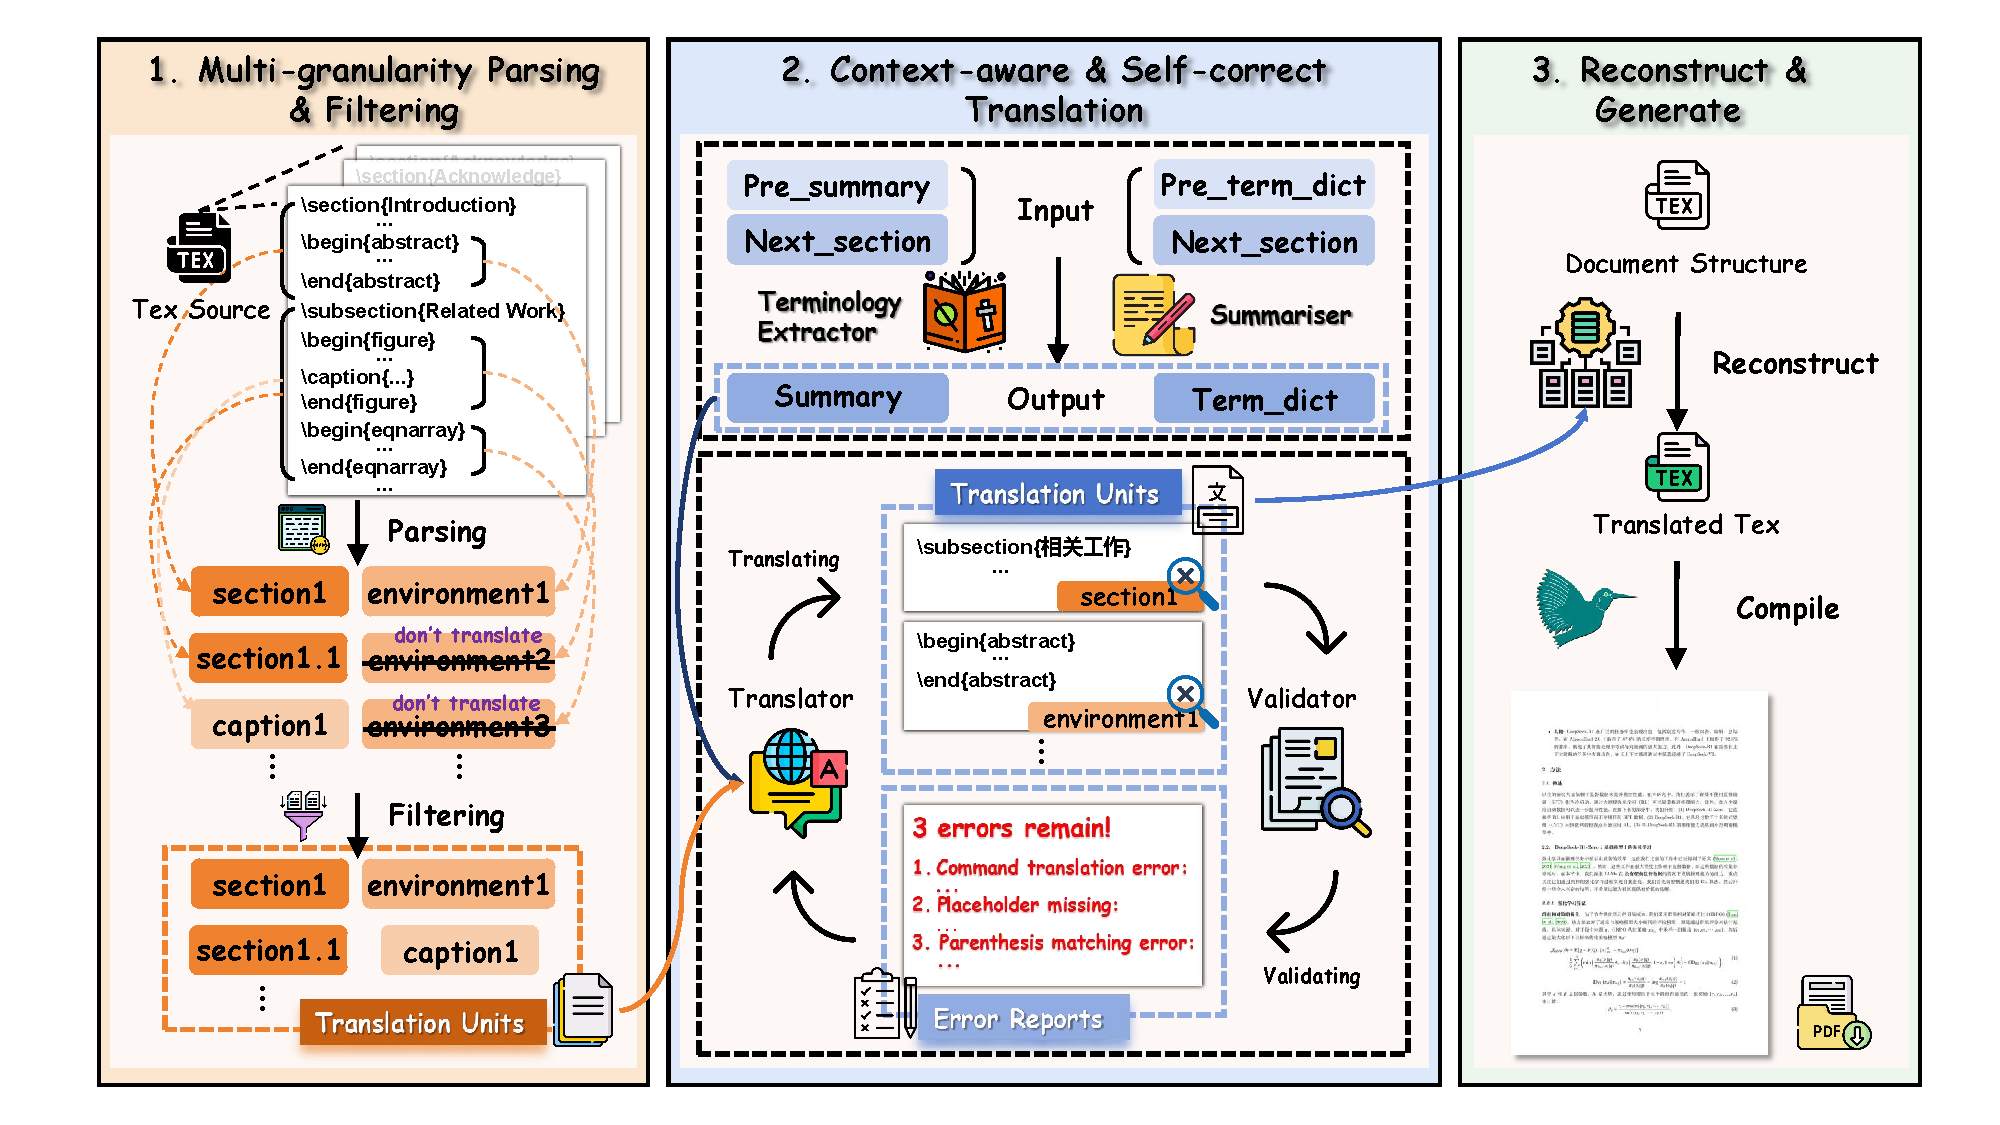
\includegraphics[width=\textwidth]{main-figure.pdf}
  \caption{بنية نظام LaTeXTrans الخاص بنا.}
  \vspace{-0.3cm}
  \label{fig:LaTeXTrans}
\end{figure*}

لتقييم فعالية LaTeXTrans، نقوم أولاً بإنشاء مجموعة اختبار مصدر LaTeX باستخدام ملفات TeX التي تم جمعها من أوراق arXiv. ثم نقارن LaTeXTrans مع مجموعة من معايير الترجمة القائمة على MT و LLM. تظهر النتائج التجريبية أن LaTeXTrans يتفوق باستمرار على جميع المعايير في كل من دقة الترجمة وأمانة التنسيق. ومن الجدير بالذكر أن LaTeXTrans يحقق تحسينًا قدره 13.20 نقطة في درجة FC، مع مكاسب كبيرة في COMETkiwi و LLM-score عند مقارنته بـ GPT-4o.
\section{الأعمال ذات الصلة}

\paragraph{ترجمة الآلة المعتمدة على LLM.}
لقد أدت ظهور LLMs إلى إدخال نموذج جديد لترجمة الآلة، حيث انتقلنا من التعلم الخاضع التقليدي على مجموعات البيانات المتوازية نحو فهم اللغة المرن وعام الاستخدام ~\citep{gain2025bridginglinguisticdividesurvey}. تظهر LLMs مثل GPT-3 ~\citep{brown2020languagemodelsfewshotlearners} و PaLM ~\citep{chowdhery2022palmscalinglanguagemodeling} و GPT-4 قدرات متعددة اللغات قوية دون تدريب صريح على مهام الترجمة. تستفيد ترجمة المعتمدة على LLM من التعلم في السياق، حيث يتم تحفيز النموذج بأمثلة أو تعليمات لأداء الترجمة بشكل فوري. وقد أظهرت هذه الطريقة أداءً تنافسياً في سيناريوهات التعلم دون عينة وقليلة العينة ~\citep{vilar2023promptingpalmtranslationassessing,luo2025decoderonlylargelanguagemodels}، خاصةً لزوج اللغات ذات الموارد العالية. على عكس الترجمة الآلية العصبية التقليدية (NMT)، التي تتطلب إعادة تدريب أو تعديل لكل مجال أو لغة جديدة، يمكن لـ LLMs التعميم عبر المهام واللغات مع الحد الأدنى من البيانات الإضافية.

\paragraph{أنظمة متعددة الوكلاء.}
مؤخراً، فتح ظهور LLMs إمكانيات جديدة لأنظمة متعددة الوكلاء (MAS). في أنظمة متعددة الوكلاء المعتمدة على LLM، يتم تجسيد كل وكيل ككيان مدعوم بـ LLM قادر على التفكير باللغة الطبيعية والتخطيط والتعاون. تظهر أنظمة مثل AutoGPT~\citep{yang2023autogptonlinedecisionmaking} و CAMEL~\citep{li2023camelcommunicativeagentsmind} و AutoGen~\citep{dibia2024autogenstudionocodedeveloper} أن وكلاء LLM يمكنهم محاكاة أدوار متنوعة وإكمال مهام معقدة من خلال التنسيق القائم على الحوار. تستكشف عدد متزايدة من الدراسات استخدام أنظمة متعددة الوكلاء لمهام متعلقة بالترجمة. ومن الجدير بالذكر أن MAS قد ظهرت كحل واعد للترجمة على مستوى الوثائق~\citep{wang2025deltaonlinedocumentleveltranslation}، وهي تحدٍ طويل الأمد في ترجمة الآلة.

\paragraph{ترجمة النصوص المنسقة.}
تنطوي ترجمة النصوص المنسقة على ترجمة الوثائق التي تحتوي على تعليمات هيكلية أو دلالية، مثل LaTeX و XML. غالباً ما تتداخل هذه الصيغ مع اللغة الطبيعية مع الأوامر أو العلامات أو الرموز التي تشفر التنسيق أو التخطيط أو التعليقات الدلالية. على الرغم من أن بعض الجهود الحديثة قد بُذلت في هذا الاتجاه~\cite{kleidermacher2025sciencelanguagesassessingllm,khan2025xmljson}، إلا أن ترجمة النصوص المنسقة لا تزال تواجه تحديين رئيسيين. الأول هو نقص نظام قوي وعام الغرض مصمم خصيصاً لترجمة المحتوى المنسق. حالياً، تقدم فقط عدد قليل من الأدوات التجارية، مثل Youdao و Baidu، حلولاً فعالة نسبياً. بينما تلقت أدوات المصدر المفتوح مثل MathTranslate\footnote{\url{https://github.com/SUSYUSTC/MathTranslate}} و GPT-Academic\footnote{\url{https://github.com/binary-husky/gpt\_academic}} تعليقات إيجابية، إلا أنها لا تزال متخلفة عن الأنظمة التجارية من حيث الأداء العام. 
الثاني هو نقص تقنية تقييم قوية لترجمة النصوص المنسقة. حيث أن درجات BLEU أو COMET التقليدية لا تغطي صحة التنسيق أو الاحتفاظ بالعلامات. لذلك، من الضروري تطوير تقنية تقييم جديدة لترجمة واعية بالهيكل.
\section{تصميم النظام}
\label{sec:system}
العمارة الأساسية لـ LaTeXTrans هي تنسيق متعدد الوكلاء مصمم لترجمة المستندات الهيكلية المكتوبة بلغة LaTeX. يتكون من ثلاث وحدات: المحلل، وحدة الترجمة، ووحدة التوليد. يتم وصف التصميم ووظائف كل مكون بالتفصيل أدناه.
\subsection{وحدة المحلل}
\label{sec:parser}
تتداخل الوثائق المصممة بلاتكس مع محتوى اللغة الطبيعية مع أوامر التنسيق وعلامات الدلالة، مما يؤدي إلى تمثيلات مترابطة بشدة ليست مناسبة للترجمة المباشرة بواسطة نماذج اللغة الكبيرة. إن تغذية الوثيقة بالكامل بشكل ساذج إلى نموذج لغة كبير يؤدي إلى عدة مشكلات: معالجة غير ضرورية للمكونات غير القابلة للترجمة، وزيادة التكلفة الحسابية، وزيادة خطر إدخال أخطاء في الترجمة. 
لمعالجة هذه التحديات، نقدم وحدة المحلل، التي تعمل كأول مرحلة في خط أنابيب LaTeXTrans. فكرتها الأساسية هي تحويل وثائق LaTeX المعقدة إلى وحدات ترجمة منظمة ونظيفة، مما يسهل على نماذج اللغة الكبيرة معالجتها. على وجه التحديد، نصمم استراتيجية استبدال العناصر النائبة لاستبدال الأوامر والبيئات الخاصة بلاتكس مؤقتًا، وننفذ آلية تصفية لإزالة المكونات التي لا تتطلب ترجمة.

\paragraph{استراتيجية استبدال العناصر النائبة.}
\begin{figure*}[!t]
  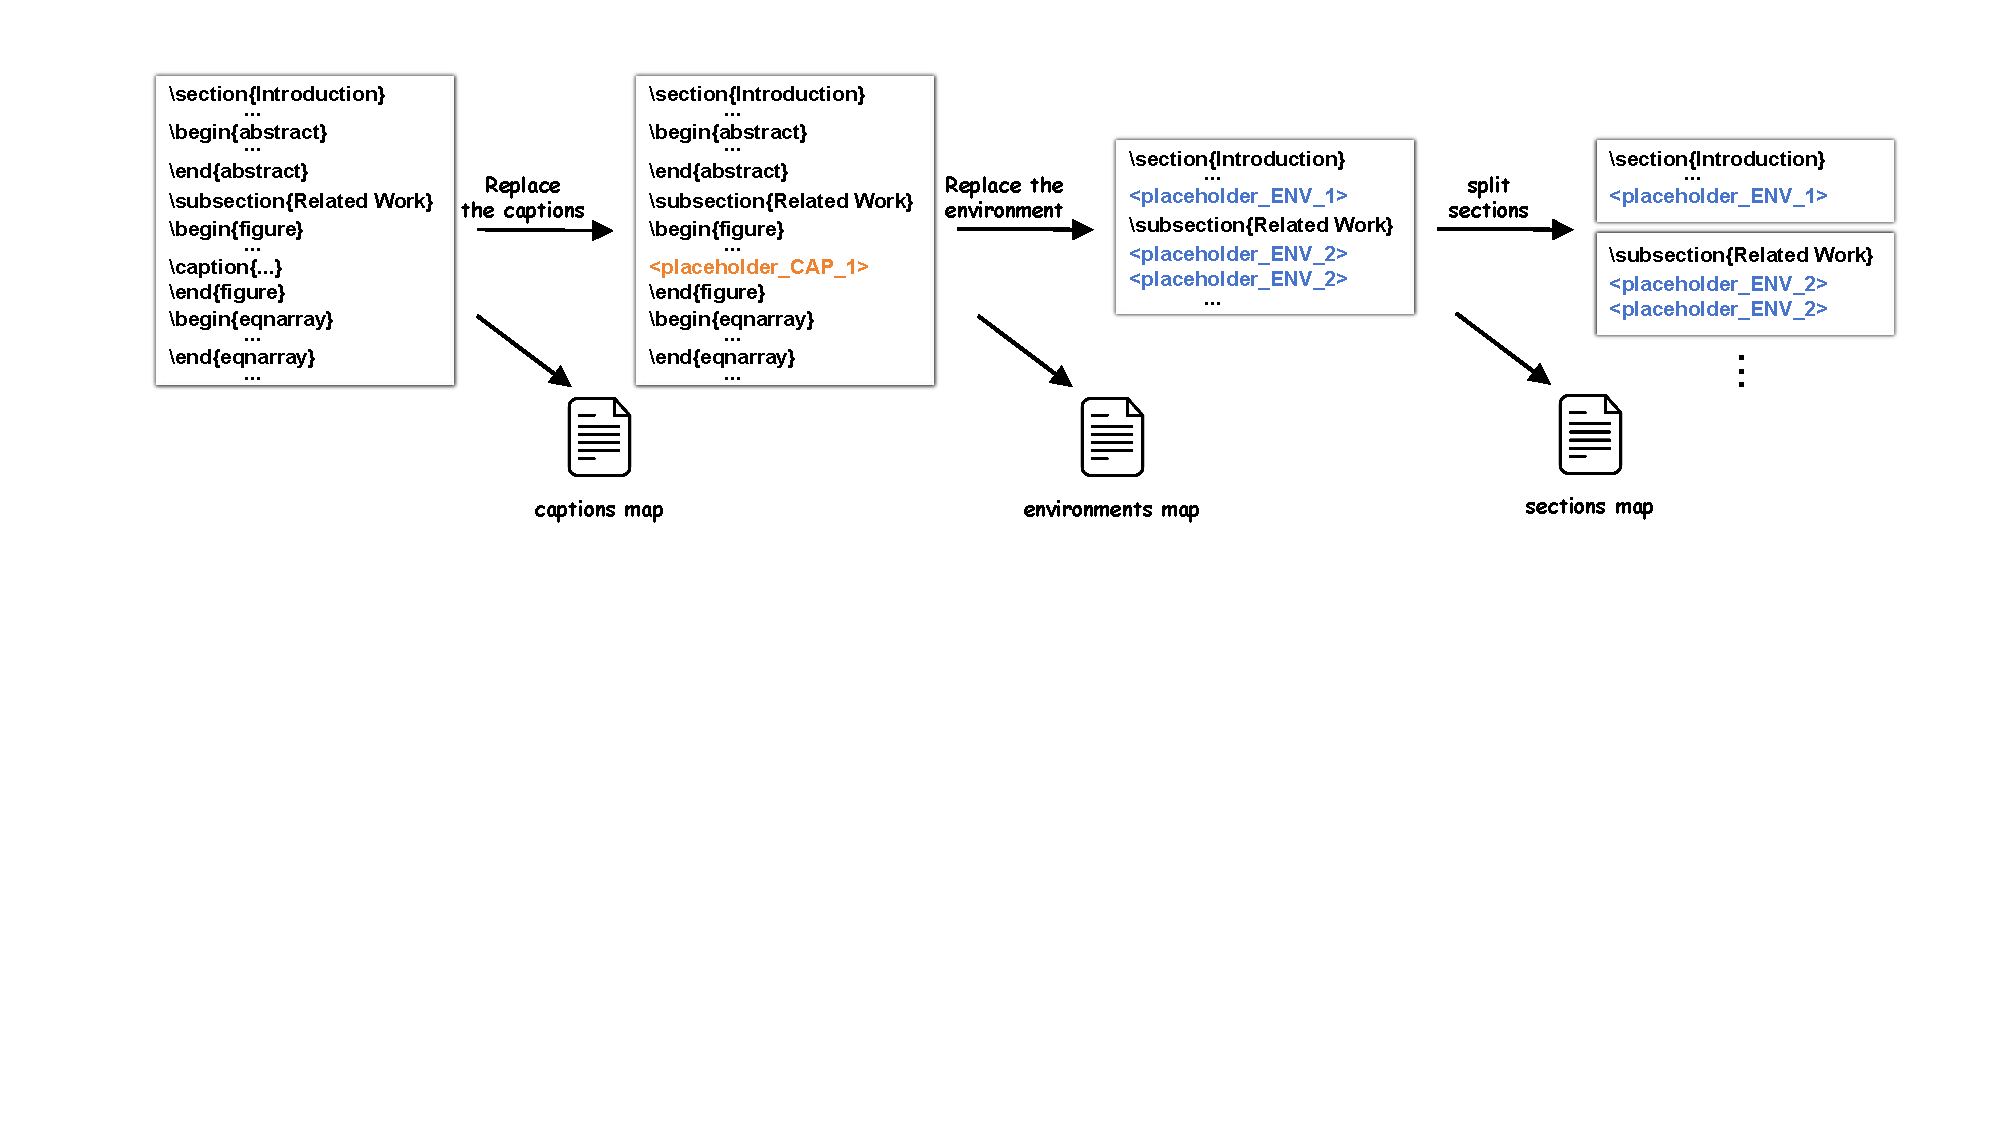
\includegraphics[width=\textwidth]{placeholder.pdf}
  \vspace{-0.7cm}
  \caption{خط الأنابيب لاستراتيجية استبدال العناصر النائبة لدينا. ملفات الربط هي الربط بين العناصر النائبة والمحتوى المستبدل، وهي أيضًا وحدات ترجمة بمستويات تجزئة مختلفة.}
  \vspace{-0.3cm}
  \label{fig:placeholder}
\end{figure*}

بالنسبة لوثيقة LaTeX الشائعة، يتم عرض استراتيجيتنا لاستبدال العناصر النائبة في الشكل \ref{fig:placeholder}. نعتبر أن الصيغ الرياضية الأصلية والمخططات محفوظة أثناء الترجمة. الخطوة الأولى هي استبدال التسميات في المخطط بعناصر نائبة. الخطوة الثانية هي استبدال البيئة بعناصر نائبة، والتي ستشمل الغالبية العظمى من الصيغ الرياضية، والمخططات، وأجزاء أخرى لا تحتاج إلى ترجمة. أخيرًا، نقوم بتقسيم النص المستبدل إلى أقسام (بما في ذلك الأقسام الفرعية والأقسام الفرعية ذات المستويات الأدنى). لمشروع LaTeX يتكون من عدة ملفات tex، نقوم أولاً بدمج الملفات اللازمة في الملف الرئيسي ثم إدراج العناصر النائبة في بداية ونهاية الدمج لاستعادة مستقبلية. قواعد استبدال العناصر النائبة وطرق التقسيم تظل كما كانت من قبل. من استراتيجية استبدال العناصر النائبة، نحصل على وحدات ترجمة ذات دقتين: السياق (أي القسم والبيئة) والجملة (أي التسمية).

\paragraph{مرشح وحدة الترجمة.}
بينما يتم استبدال المكونات غير القابلة للترجمة بعناصر نائبة، نلاحظ أن LaTeX يسمح للمستخدمين بتعريف بيئات مخصصة، مما يجعل من غير الممكن الاعتماد فقط على نهج قائم على القواعد الشاملة لتحديد جميع هذه المقاطع. لمعالجة هذه المشكلة، نكمل قائمة محددة مسبقًا من البيئات المحمية مع وكيل تصفية مدعوم بنموذج لغة كبير، والذي يحدد ديناميكيًا ما إذا كانت البيئة المعطاة تتطلب ترجمة. يتم وضع علامة ثنائية على كل بيئة مستخرجة: \texttt{True} أو \texttt{False}. بعد ذلك، تعالج وحدة الترجمة فقط تلك المقاطع المعلّمة بـ \texttt{True}.
\subsection{وحدة الترجمة}
تتكون وحدة الترجمة من أربعة عناصر: المترجم، المدقق، الملخص، ومُستخرج المصطلحات. بعد أن يُكمل المترجم ترجمة جميع الوحدات المعينة، يتم تمرير الناتج إلى المدقق، الذي يُولد تقريرًا عن الأخطاء ويُعيده للتعديل إذا لزم الأمر. يساعد الملخص ومُستخرج المصطلحات المترجم من خلال توفير ملخص للمحتوى السابق وقاموس مصطلحات متخصص في المجال، مما يعزز من التماسك السياقي ويضمن اتساق المصطلحات طوال عملية الترجمة.
\label{sec:transandval}

\paragraph{تكرار المترجم والمدقق.}
عند استخدام نوافذ سياقية كبيرة لترجمة الوثائق، غالباً ما تُفضل نماذج اللغة الكبيرة (LLMs) التقاط المعنى العام للنص، مما يمكن أن يؤدي إلى إغفال أو سوء ترجمة الجمل الفردية~\cite {wang2025deltaonlinedocumentleveltranslation}. وتكون هذه المشكلة واضحة بشكل خاص في ترجمة وثائق LaTeX، حيث قد تتجاهل نماذج اللغة الكبيرة أو تُترجم بشكل غير صحيح أوامر LaTeX. على سبيل المثال، قد يتم إغفال الأمر ``\texttt{\textbackslash textbf\{\}}''، أو قد يتم ترجمة ``\texttt{\textbackslash left}'' بشكل غير صحيح كـ ``\begin{CJK}{UTF8}{gbsn}\texttt{\textbackslash 左}\end{CJK}''.
نظرًا للبنية الحساسة والموضوعة لـ LaTeX، فإن مثل هذه الأخطاء شائعة ويمكن أن تؤدي إلى فشل في الترجمة. لمعالجة هذه المشكلة، نقدم إطار عمل تكراري بين المترجم والمدقق، يقوم بإجراء عدة جولات من التحقق لتحسين الحفاظ على أوامر LaTeX لكل وحدة ترجمة. يعزز هذا التحسين التكراري بشكل كبير قابلية الاستخدام وموثوقية نظام الترجمة الكلي. على وجه التحديد، كما هو موضح في الشكل \ref{fig:LaTeXTrans}، بعد أن يُكمل المترجم ترجمة جميع وحدات الترجمة، سيتحقق المدقق من جودة الترجمة من ثلاثة أبعاد وسينتج في النهاية تقريرًا عن الأخطاء. عند إجراء الجولة التالية من الترجمة، ستشكل وحدات الترجمة الخاطئة، مع تقارير الأخطاء، المحفز للمترجم لإرشادهم في توليد الترجمة الصحيحة.

\paragraph{الملخص ومُستخرج المصطلحات.}
مستوحاة من عمل \citet{wang2025deltaonlinedocumentleveltranslation}، نقوم بتصميم ملخص ومُستخرج مصطلحات لتعزيز التماسك السياقي واتساق المصطلحات في الترجمة. على وجه التحديد، يتحمل الملخص مسؤولية توليد وتحديث ملخص النص السابق باستمرار خلال عملية الترجمة. عند الانتهاء من كل وحدة ترجمة، سيقوم الملخص بدمج الملخص السابق مع النص الأصلي لوحدة الترجمة الحالية لتوليد ملخص جديد. يتحمل مُستخرج المصطلحات مسؤولية الحفاظ على قاموس المصطلحات وإضافته إلى المحفز الخاص بالمترجم لتوفير مرجع لترجمة المصطلحات للمترجم. عند انتهاء المترجم من ترجمة وحدة ترجمة، يقوم مُستخرج المصطلحات باستخراج أزواج المصطلحات من النص الأصلي والترجمة ويقوم بتحديث قاموس المصطلحات في الوقت الحقيقي.
\subsection{وحدة التوليد}
وحدة التوليد مسؤولة عن إعادة تجميع وحدات الترجمة في مستندات LaTeX منظمة وتجميع مستندات LaTeX المنظمة إلى ملفات PDF باستخدام أدوات تجميع محددة (مثل pdf\LaTeX{} و Xe\LaTeX{}).
\section{تجربة}
\label{sec:experiment}

\begin{table*}[!t]
  \small
  \setlength{\tabcolsep}{2.5pt}
  \centering
  \resizebox{\textwidth}{!}{
  \begin{tabular}{lcccccccc}
  \midrule
  \multirow{2}{*}{\textbf{System}} &
  \multicolumn{4}{c}{\textbf{En-Zh}}  &
  \multicolumn{4}{c}{\textbf{En-Ja}}
  \\
  \cmidrule(l){2-5} \cmidrule(l){6-9}
  &   \bf Cometkiwi ($\uparrow$) & \bf LLM-score ($\uparrow$) & \bf FC-score ($\uparrow$)  & \bf Cost ($\downarrow$)  & \bf Cometkiwi ($\uparrow$) & \bf LLM-score ($\uparrow$) & \bf FC-score ($\uparrow$)  & \bf Cost ($\downarrow$) \\
    \midrule
    NiuTrans               &64.69    &7.93     & 60.72     &-   &65.49          &8.19     & 27.48      &-      \\
    Google Translate                           &46.23  &5.93        & 51.00      &-   &56.21           &7.01     & 50.00      &-     \\
    \hdashline
    LLaMA-3.1-8b                       &42.89     &2.92     &49.40   &-   &44.49           &3.32     &60.92  &-     \\
    Qwen-3-8b              &45.55    &7.87    &48.68   &-   &46.20        &6.80     &49.52      &-     \\
    Qwen-3-14b         &68.18 &8.76 &65.63 &- &72.84 &8.66 &61.88 &-       \\
    \hdashline
    DeepSeek-V3              & 67.26    & \textbf{9.02}      & 63.68    & \$\bf0.02   & 72.17        & \textbf{9.00}     &63.96      & \$\bf0.03     \\
    GPT-4o                      & 67.22    & 8.58   & 58.32    & \$0.13    &71.16     &8.91      &56.92   & \$0.11  \\
    \hdashline
    LaTeXTrans\textsubscript{Qwen-3-14b}         &71.37      &8.97      &71.20   &-     &74.68     &8.51      &59.84   &-  \\
    LaTeXTrans\textsubscript{DeepSeek-V3}         &73.48      & 9.01       &70.52   & \$0.10     &\textbf{75.39}     &8.89      &\textbf{66.52}   &\$0.13  \\
    LaTeXTrans\textsubscript{GPT-4o}               &\textbf{73.59}      & 8.92       &\textbf{71.52}    & \$0.35   &74.47     &8.93      &64.92   &\$0.45  \\
  \midrule
\end{tabular}}
\vspace{-0.3cm}
\caption{
مقارنات COMETkiwi و FC-score و LLM-score عبر أنظمة مختلفة. كما نبلغ عن التكلفة المتكبدة عند استخدام واجهة برمجة التطبيقات الرسمية لترجمة كل ورقة في المتوسط في مجموعة الاختبار، كما هو موضح في عمود "التكلفة". \textbf{Bold} يشير إلى أفضل نتيجة في كل مجموعة.
}
\vspace{-0.4cm}
\label{tab:main-results}
\end{table*}
\subsection{الإعدادات}
\paragraph{مجموعة البيانات.}
نظرًا لعدم وجود مجموعة بيانات وثائق LaTeX متاحة للجمهور حاليًا، قمنا بإنشاء مجموعة الاختبار الخاصة بنا عن طريق اختيار مصادر TeX لـ 50 ورقة أكاديمية باللغة الإنجليزية من مستودع arXiv. تشمل الأوراق المختارة مقالات طويلة وقصيرة، العديد منها يحتوي على صيغ معقدة وأشكال، مما يضمن تنوعًا هيكليًا وتعقيدًا في محتوى LaTeX. 
تفاصيل تجريبية إضافية موضحة في الملحق~\ref{app:detailed-settings}.

\paragraph{الأسس.}
تُصنَّف أسسنا إلى مجموعتين: أنظمة الترجمة التقليدية وأنظمة الترجمة المستندة إلى LLM. بالنسبة للأولى، اخترنا NiuTrans و Google Translate كنظم تمثيلية. بالنسبة للأخيرة، قمنا بتقييم خمسة نماذج LLM قوية، تشمل كلًا من النماذج مفتوحة المصدر والنماذج التجارية: LLaMA-3.1-8B \cite{grattafiori2024llama}، Qwen-3-8B \cite{yang2025qwen3}، Qwen-3-14B، DeepSeek-V3 \cite{liu2024deepseek}، و GPT-4o \cite{hurst2024gpt}. من بين هذه النماذج، تم استخدام Qwen-3-14B و DeepSeek-V3 و GPT-4o كنماذج أساسية للوكلاء في LaTeXTrans.
\subsection{مقاييس التقييم}
قمنا بإجراء تقييم شامل لنظامنا من بعدين: جودة الترجمة وقدرة الاحتفاظ بالتنسيق.
\paragraph{جودة الترجمة.}
نظرًا لأن الترجمات المرجعية عالية الجودة لوثائق LaTeX تتطلب تعليماً على مستوى الخبراء، اعتمدنا على wmt22-cometkiwi-da~\cite{rei2022cometkiwiistunbabel2022submission}، وهو مقياس تقييم بدون مرجع (يشار إليه بـ \textit{Cometkiwi})، لتقييم جودة ترجمة وثائق LaTeX. علاوة على ذلك، استخدمنا GPT-4o كمقيّم تلقائي لتقييم جودة الترجمة عبر أبعاد متعددة، مسترشدين بمطالبات نظام مصممة بعناية. شمل التقييم أربعة جوانب: الأمانة، والطلاقة، وتناسق المصطلحات، والتماسك، حيث تم تقييم كل منها على مقياس من 0 إلى 10. ثم تم تجميع درجة عامة بواسطة GPT-4o بناءً على الدرجات الفردية عبر هذه الأبعاد (يشار إليها بـ \textit{LLM-score}).
\paragraph{قدرة الاحتفاظ بالتنسيق.}
ما إذا كانت التسميات محتفظ بها بالكامل هو تجسيد مهم لقدرة نظام ترجمة النص المنسق. ومع ذلك، في الوقت الحالي، لا يوجد مؤشر عالمي لتقييم قدرة الاحتفاظ بالتنسيق للنماذج أو الأنظمة خلال عملية الترجمة. لذلك، لوثائق LaTeX، صممنا مقياس تقييم جديد، \textbf{\underline{F}}قدرة \textbf{\underline{الاحتفاظ}} \textbf{\underline{بالتنسيق}} (يشار إليه بـ \textit{FC-score})، لتقييم قدرة نظامنا على الاحتفاظ بتسميات LaTeX خلال عملية الترجمة. يمكننا حساب FC-score عن طريق
\begin{eqnarray}
\text{FC-score} = S_0 - \alpha N_{e} - \beta N_{w} + \gamma C
\end{eqnarray}
حيث $S_0$ هو الدرجة الأولية قبل المكافآت والعقوبات، $\alpha$ هو معامل العقوبة لكل خطأ، $\beta$ هو معامل العقوبة لكل تحذير، $\gamma$ هو المكافأة للتجميع الناجح. $N_{e}$ و $N_{w}$ هما عدد الأخطاء والتحذيرات، $C \in \{0, 1\}$ يشير إلى ما إذا كانت وثيقة LaTeX قد تم تجميعها بنجاح. ثم نقوم بقص الدرجة إلى النطاق الصالح $[S_{\min}, S_{\max}]$، حيث $S_{\max}$ و $S_{\min}$ هما الحد الأعلى والحد الأدنى للدرجة (على سبيل المثال 0\textasciitilde100).

\begin{figure*}[t]
  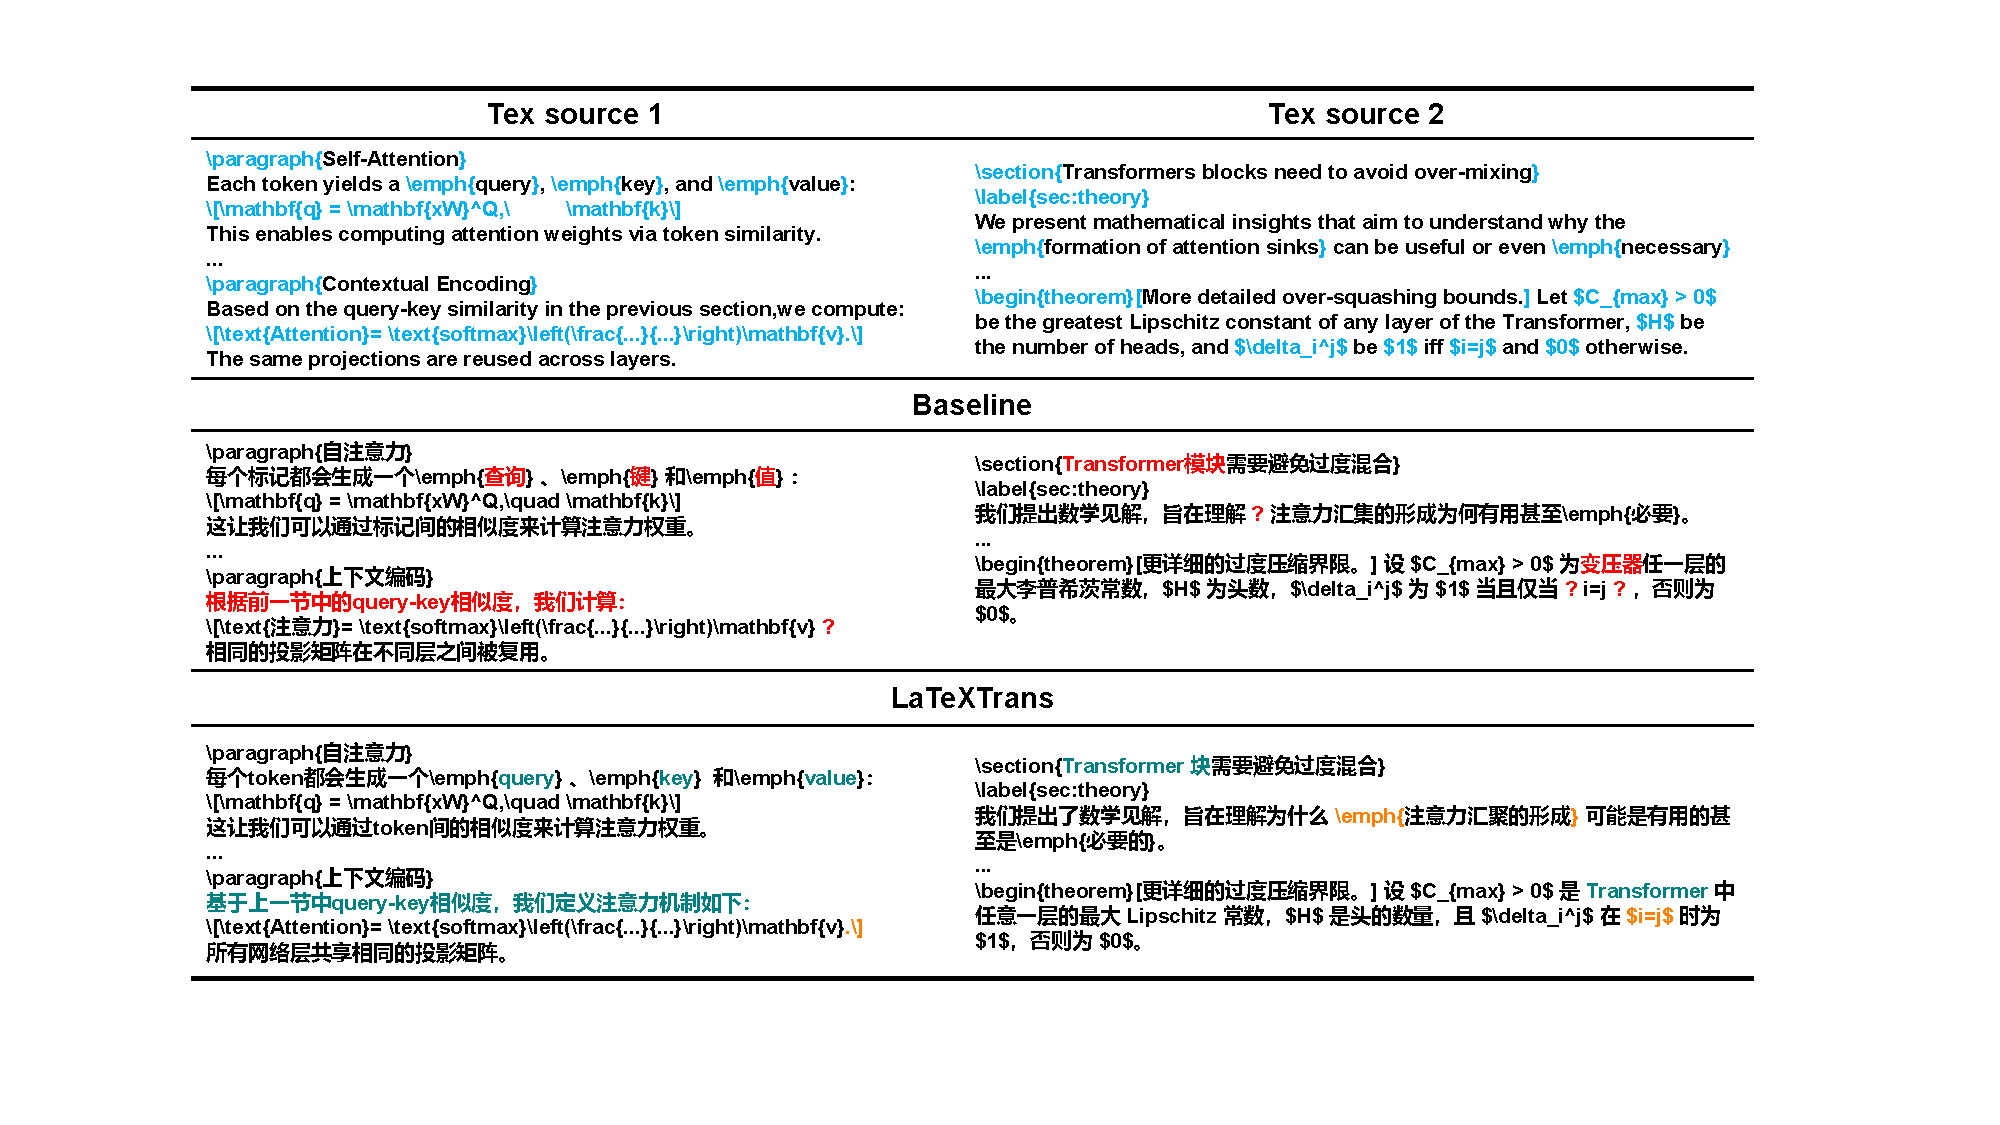
\includegraphics[width=\textwidth]{case-study-main.pdf}
  \vspace{-0.7cm}
  \caption{
    مقارنة جودة الترجمة في حالتين تمثيليتين بين الأساس و LaTeXTrans.
    في مصدر LaTeX، \textbf{\color{myblue}{الأزرق}} يميز النصوص التي يجب الحفاظ عليها. علامة استفهام حمراء (``\textbf{\color{red}{?}}'') تشير إلى فقدان العلامات أثناء الترجمة.
    \textbf{\color{red}{الأحمر}} يبرز الترجمات غير المتسقة، \textbf{\color{teal}{الأخضر}} يشير إلى الترجمات المتسقة، و \textbf{\color{orange}{البرتقالي}} يظهر العلامات LaTeX التي فاتت من الأساس ولكن تم الحفاظ عليها بنجاح بواسطة LaTeXTrans.
}
  \vspace{-0.2cm}
  \label{fig:casestudy}
\end{figure*}
\subsection{النتائج}
نقوم بتقييم نظام LaTeXTrans لدينا على مهمتين للترجمة: الإنجليزية إلى الصينية (En-Zh) والإنجليزية إلى اليابانية (En-Ja). تظهر النتائج، الموضحة في الجدول~\ref{tab:main-results}، أن LaTeXTrans يتفوق باستمرار على كل من معايير NMT وSingle-Agent عبر جميع مقاييس التقييم، بما في ذلك COMETkiwi وFC-score. من حيث جودة الترجمة، يظهر LaTeXTrans تحسينات كبيرة في FC-score (71.52 مقابل 58.32 لمهمة En-Zh و70.52 مقابل 63.68 لمهمة En-Ja)، مما يشير إلى الحفاظ بشكل أفضل على تنسيق LaTeX أثناء الترجمة. علاوة على ذلك، عندما يتم دعمه بواسطة GPT-4o كنموذج أساسي، يحقق LaTeXTrans أعلى الدرجات عبر جميع مقاييس التقييم الثلاثة—COMETkiwi وLLM-score وFC-score—مؤكداً أدائه القوي العام في الترجمة على الوثائق المنظمة بتنسيق LaTeX. من حيث تكلفة الترجمة، يقدم LaTeXTrans أداءً متفوقاً دون تكبد زيادة كبيرة في النفقات الحاسوبية مقارنة بأنظمة الترجمة الأخرى المعتمدة على LLM، مما يجعله مناسبًا للنشر على نطاق واسع في التطبيقات الواقعية.
\subsection{دراسة الإلغاء}
Table~\ref{tab:ablation} presents an ablation study on the En–Zh task using GPT-4o and DeepSeek-V3 as backbone models. Introducing the Parser module significantly improves both COMETkiwi and FC-score, indicating that the placeholder substitution strategy enhances translation quality and label preservation. Adding the Validator module further boosts overall performance, although a slight drop in LLM-score is observed with DeepSeek-V3. We hypothesize that this is due to the Validator enforcing strict tag retention through iterative checks, which may restrict the Translator and slightly impact fluency. Finally, incorporating the Summarizer and Terminology Extractor improves the LLM-score, reflecting better cross-paragraph coherence. However, slight declines in COMETkiwi and FC-score suggest that these improvements may not be fully captured by COMETkiwi. A detailed analysis with a case study is provided in Section~\ref{sec:translation-consistency}.

\begin{table}[t]
  \setlength{\tabcolsep}{1.5pt}
  \small
  \centering
  \resizebox{\columnwidth}{!}{
  \begin{tabular}{lcccccc}
  \toprule
  \multirow{2}{*}{\textbf{Setting}} & \multicolumn{3}{c}{\textbf{GPT-4o}}  & \multicolumn{3}{c}{\textbf{DeepSeek-V3}} \\
  \cmidrule(r){2-4} \cmidrule(r){5-7}
  & \bf Cometkiwi & \bf LLM-score & \bf FC-score  & \bf Cometkiwi & \bf LLM-score & \bf FC-score  \\
  \midrule
  SA. (Baseline)                & 67.22 & 8.58 & 58.32  & 67.26 & 9.02 & 63.68  \\  \hdashline
  SA. + P.           & 74.47 & 8.89 & 69.64  & 74.39 & 9.03 & 70.08  \\
  SA. + P. + V.      & \textbf{74.57} & 8.91  & \textbf{71.76}   & \textbf{74.42} & 8.94 & \textbf{70.80}  \\
  SA. + P. + V. + S. & 74.06  & \textbf{8.95}  & 71.64  & 74.02 & \textbf{9.05} & 70.68  \\
  SA. + P. + V. + S. + TE.  & 73.59 & 8.93 & 71.52  & 73.48 & 9.01 & 70.52  \\
  \bottomrule
  \end{tabular}
  }
  \caption{
  أداء LaTeXTrans مع إعدادات مختلفة.
  ``SA.'' تشير إلى قاعدة الترجمة المعتمدة على LLM، ``P.'' تعني المحلل، ``V.'' تعني المدقق، ``S.'' تعني الملخص، و``TE.'' تعني مستخرج المصطلحات.  ``SA. + P. + V. + S. + TE.'' تتوافق مع LaTeXTrans لدينا.
}
  \vspace{-0.4cm}
  \label{tab:ablation}
\end{table}
\subsubsection{اتساق الترجمة}
\label{sec:translation-consistency}
نقدم دراسة حالة لمهمة إن-ص من مجموعة الاختبار لدينا لإظهار أن نظامنا يؤدي بالفعل بشكل أفضل من حيث اتساق الترجمة، كما هو موضح في الشكل~\ref{fig:casestudy}. في هذه الحالة، تبقى ترجمة المصطلحات من LaTeXTrans متسقة عبر الأقسام الثلاثة. في المقابل، تجد الطريقة الأساسية صعوبة في الحفاظ على مثل هذا الاتساق. وهذا يشير إلى أن نظامنا يمكنه الحفاظ على اتساق ممتاز طوال عملية الترجمة بأكملها.

\vspace{-0.1cm}
\section{الخاتمة}
في هذه الورقة، نقترح LaTeXTrans، نظام متعدد الوكلاء لترجمة الوثائق المنظمة بتنسيق LaTeX. يتكون LaTeXTrans من ثلاثة وحدات تعاونية، كل منها مسؤول عن مرحلة معينة من عملية الترجمة. تظهر النتائج التجريبية أن LaTeXTrans يمكن أن يتفوق على الأنظمة الأساسية ويقدم حلاً موثوقًا لترجمة وثائق LaTeX.
\section*{القيود}
يمكن دمج أي نموذج لغة يتبع التعليمات في نظام LaTeXTrans الخاص بنا. ومع ذلك، نظرًا لعدد النماذج المتاحة الكبير، فإنه من غير العملي تقييم كل نموذج بشكل فردي. لذلك، نختار مجموعة تمثيلية من نماذج LLM الشائعة الاستخدام لتجاربنا. نحن نعتقد أن هذا الاختيار يوضح بشكل كافٍ قابلية التطبيق وفاعلية LaTeXTrans في ترجمة مستندات LaTeX. بالإضافة إلى ذلك، على الرغم من أن الأنظمة التجارية مثل Baidu و Youdao تقدم خدمات ترجمة LaTeX، إلا أنها ليست مفتوحة المصدر. نتيجة لذلك، لا يمكننا حساب مقاييس مثل COMETkiwi و FC-score لهذه الأنظمة. لذلك، لا نقوم بتضمين مقارنة شاملة معها في تجاربنا الرئيسية.

\bibliography{custom}

\appendix
\clearpage
\section{الإعدادات التفصيلية الإضافية للتجربة}
\label{app:detailed-settings}

\paragraph{الأسس.}
نظرًا لأن مجموعة البيانات تتكون بالكامل من مستندات LaTeX هيكلية تفوق قدرات الأنظمة ذات النموذج الواحد، اعتمدنا خطوة معالجة مسبقة في النهج الأساسي. على وجه التحديد، تم تقسيم مستندات LaTeX الهيكلية إلى وحدات ترجمة على مستوى الأقسام لجعلها قابلة للإدارة للترجمة.

\paragraph{إعدادات المعلمات الفائقة.}
في التجارب، قمنا بتقييم كل من النماذج مفتوحة المصدر والنماذج مغلقة المصدر بشكل منفصل. بالنسبة للنماذج مغلقة المصدر، قمنا بالوصول إليها عبر واجهة برمجة تطبيقات طرف ثالث. في النهج الأساسي، قمنا بتعيين الحد الأقصى لعدد الرموز الجديدة إلى 16,384 ودرجة الحرارة إلى 0.7، مع الاحتفاظ بجميع المعلمات الفائقة الأخرى عند قيمها الافتراضية. بالنسبة لنظامنا، تم تعيين درجة الحرارة في الفلتر إلى 0 مع حد أقصى يبلغ 50 رمزًا جديدًا، في حين تم تكوين جميع الوكلاء الآخرين بحد أقصى يبلغ 8,192 رمزًا جديدًا؛ وتم الاحتفاظ بالمعلمات الفائقة المتبقية عند قيمها الافتراضية.

\paragraph{التقييم.}
عند حساب درجات COMETkiwi وLLM، استخدمنا \texttt{pylatexenc}\footnote{\url{https://github.com/phfaist/pylatexenc}} لتحويل كل وحدة ترجمة LaTeX إلى نص عادي. على الرغم من أن LaTeXTrans يقوم بتحليل مستندات LaTeX الهيكلية إلى وحدات ترجمة دقيقة، إلا أننا اتبعنا بروتوكول التقييم الخاص بالأساس باستخدام وحدات ترجمة على مستوى الأقسام لحساب كل من درجات COMETkiwi وLLM. علاوة على ذلك، لتقييم الاتساق السياقي في تقييم LLM، قمنا بدمج وحدات الترجمة على مستوى الأقسام في فقرات زوجية ثم قمنا بتقييمها باستخدام GPT-4o. يتم توضيح قالب الطلب المستخدم للتقييم في الشكل~\ref{fig:llmscoreprompt}. عند حساب درجة FC، قمنا بتعيين الدرجة الأولية $S_0$ إلى 100. نظرًا لأن الأخطاء لها تأثير أكبر على تأثير جدولة تنسيق PDF النهائي مقارنة بالتحذيرات، في التجربة، قمنا بتعيين القيمة لـ $\alpha$ (10) لتكون أكبر بكثير من $\beta$ (2). في النهاية، ما إذا كانت عملية التجميع ناجحة هو العامل الأكثر وضوحًا لتقييم التجميع. لذلك، في التجربة، قمنا بتعيين $\gamma$ إلى 20.

\paragraph{مجموعات البيانات}
اخترنا ملفات المصدر LaTeX لـ 50 ورقة أكاديمية في مجال علوم الكمبيوتر من arXiv كمجموعة اختبار لدينا. يتم عرض توزيع أطوال الأوراق في الشكل~\ref{fig:test-set-word-count}. بالإضافة إلى ذلك، قمنا بتحليل مواضيع الأوراق وتصويرها كسحابة كلمات في الشكل~\ref{fig:test-set-topic}. تظهر هذه النتيجة أن مجموعة الاختبار تعرض مجموعة متنوعة من أطوال الأوراق، تغطي كل من الوثائق القصيرة والطويلة، مما يساعد على ضمان القوة عبر أحجام الوثائق المختلفة. علاوة على ذلك، تكشف سحابة الكلمات عن مجموعة واسعة من مواضيع البحث ضمن مجال علوم الكمبيوتر، مما يؤكد تنوع الموضوعات في مجموعة الاختبار ويعزز عمومية تقييمنا.

\begin{figure}[h]
    \centering
    \resizebox{0.45\textwidth}{!}{
    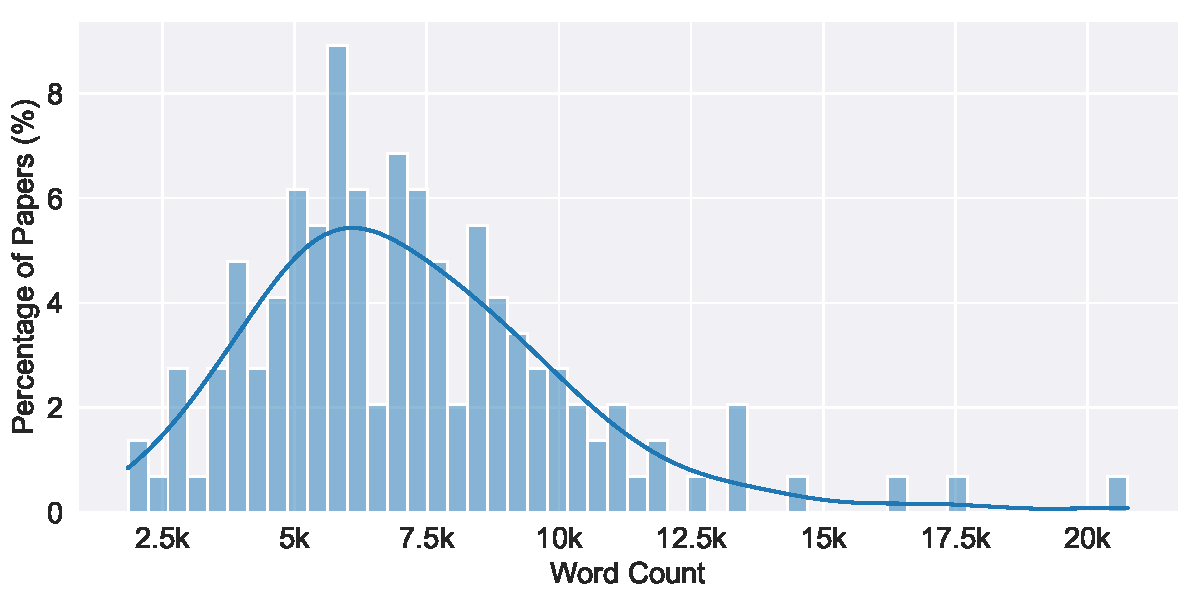
\includegraphics[width=\textwidth]{my_distribution_plot_k_labels.pdf}}
    \caption{توزيع أطوال الأوراق (بعدد الكلمات) في مجموعة الاختبار لدينا.}
    \label{fig:test-set-word-count}
\end{figure}

\begin{figure}[h]
    \centering
    \resizebox{0.45\textwidth}{!}{
    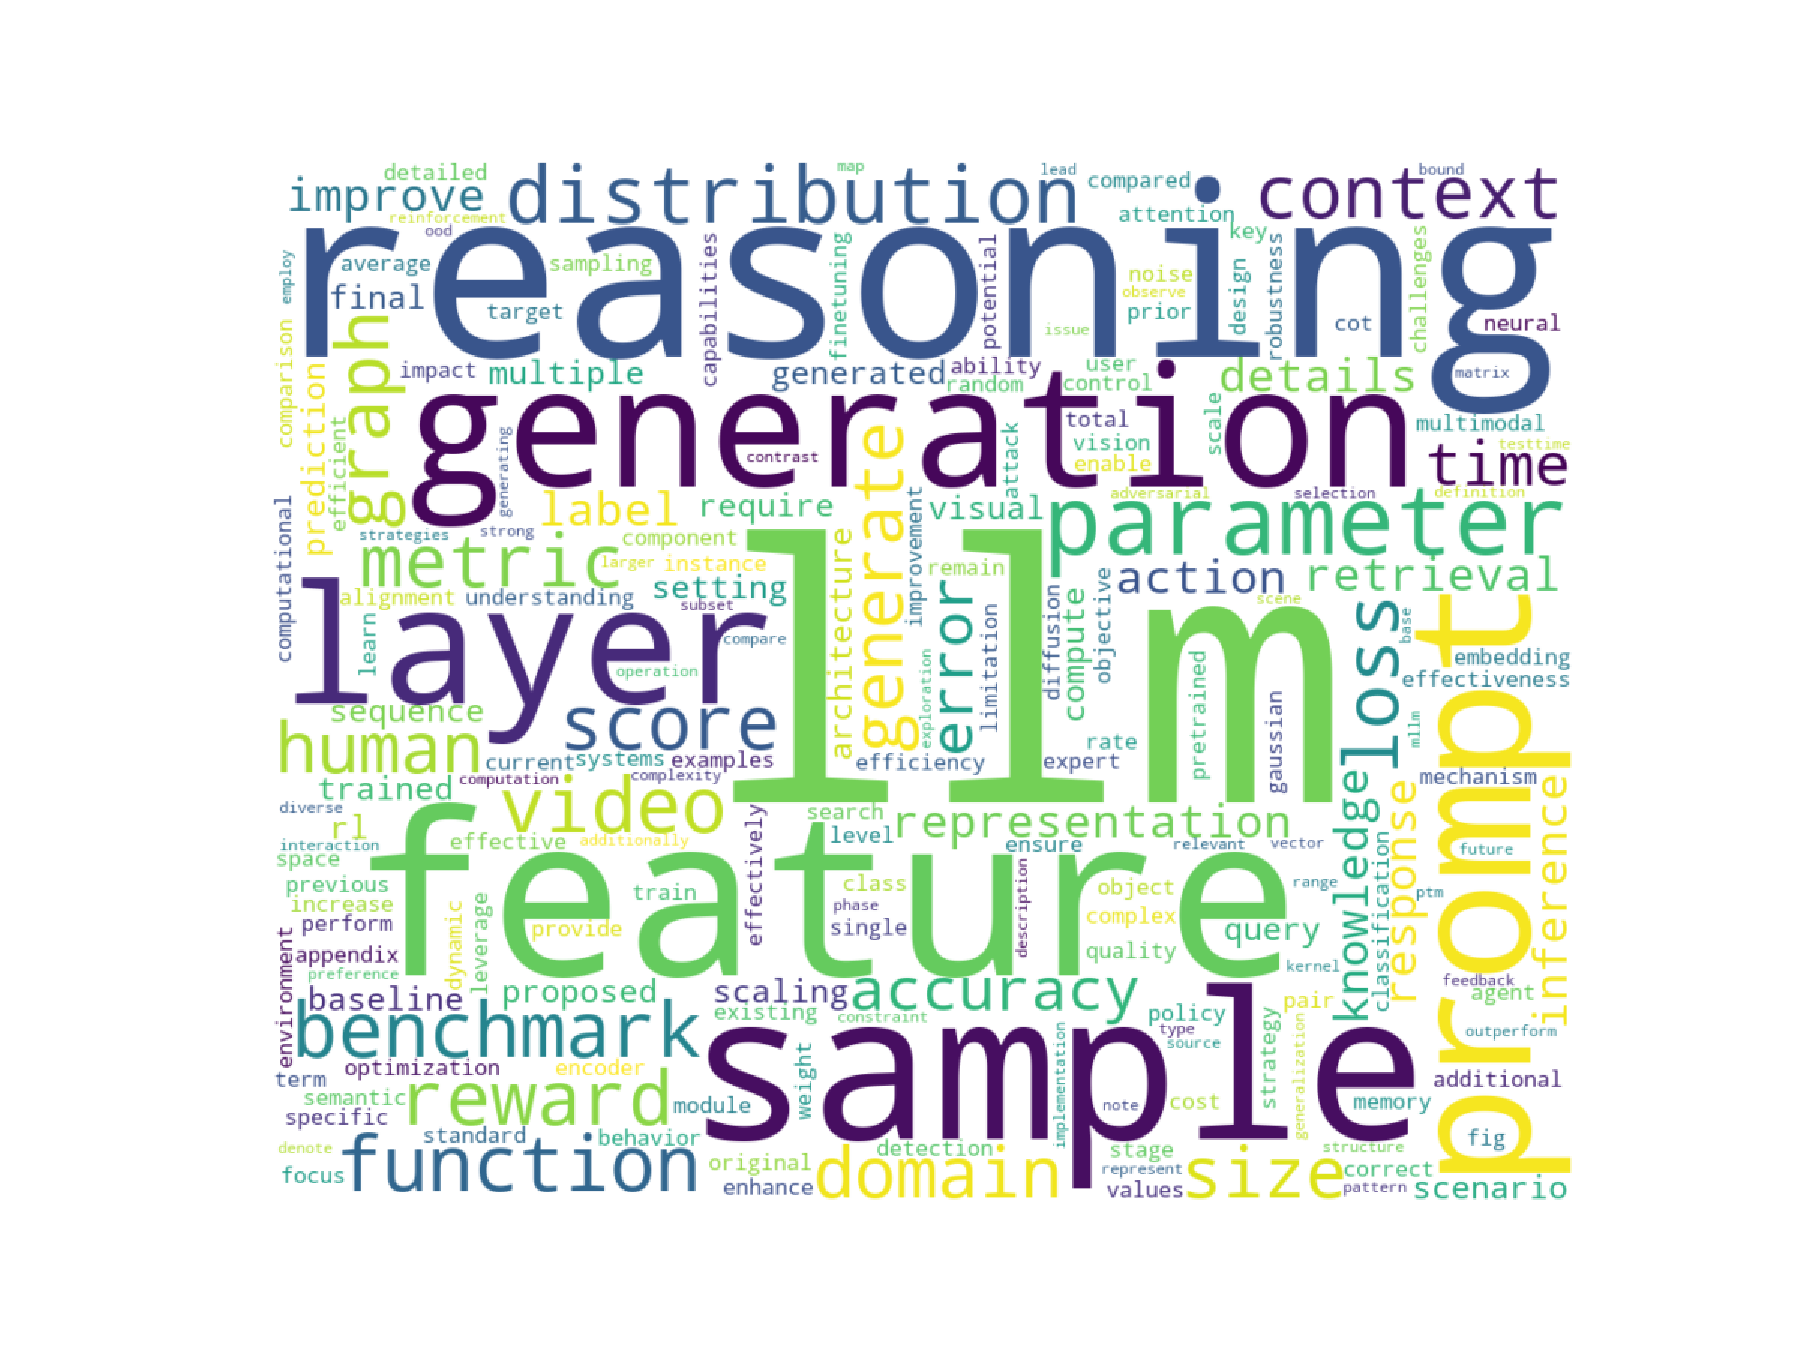
\includegraphics[width=\textwidth]{word_cloud.pdf}}
    \caption{تصوير سحابة الكلمات للمواضيع التي تم تناولها في مجموعة الاختبار الخاصة بنا.}
    \label{fig:test-set-topic}
\end{figure}
\section{عرض أداء النظام}
نختار ست حالات لعرض الأداء الترجمى لنظامنا بصريًا، مع التركيز على مهام الترجمة من الإنجليزية إلى الصينية ومن الإنجليزية إلى اليابانية، كما هو موضح في الشكل~\ref{fig:case1} إلى الشكل~\ref{fig:case6}. جميع الحالات الست هي حالات ترجمة لشفرة المصدر LaTeX لمقالات بواسطة LaTeXTrans. في كل حالة، اخترنا جزئين معقدين نسبيًا لعرضهما. من بين الحالات الست، هناك ثلاث مهام ترجمة من الإنجليزية إلى الصينية وثلاث مهام ترجمة من الإنجليزية إلى اليابانية، على التوالي.
\section{قوالب الطلبات لمكونات قائمة على LLM في LaTeXTrans}
\label{sec:prompts}
تظهر الأشكال~\ref{fig:translator prompt 1} إلى~\ref{fig:template-for-summarizer} قوالب الطلبات المستخدمة من قبل الوكلاء داخل نظام LaTeXTrans.

\clearpage
\par
\begin{figure*}[!t]
    \centering
    \begin{subfigure}[t]{0.48\textwidth}
        \centering
        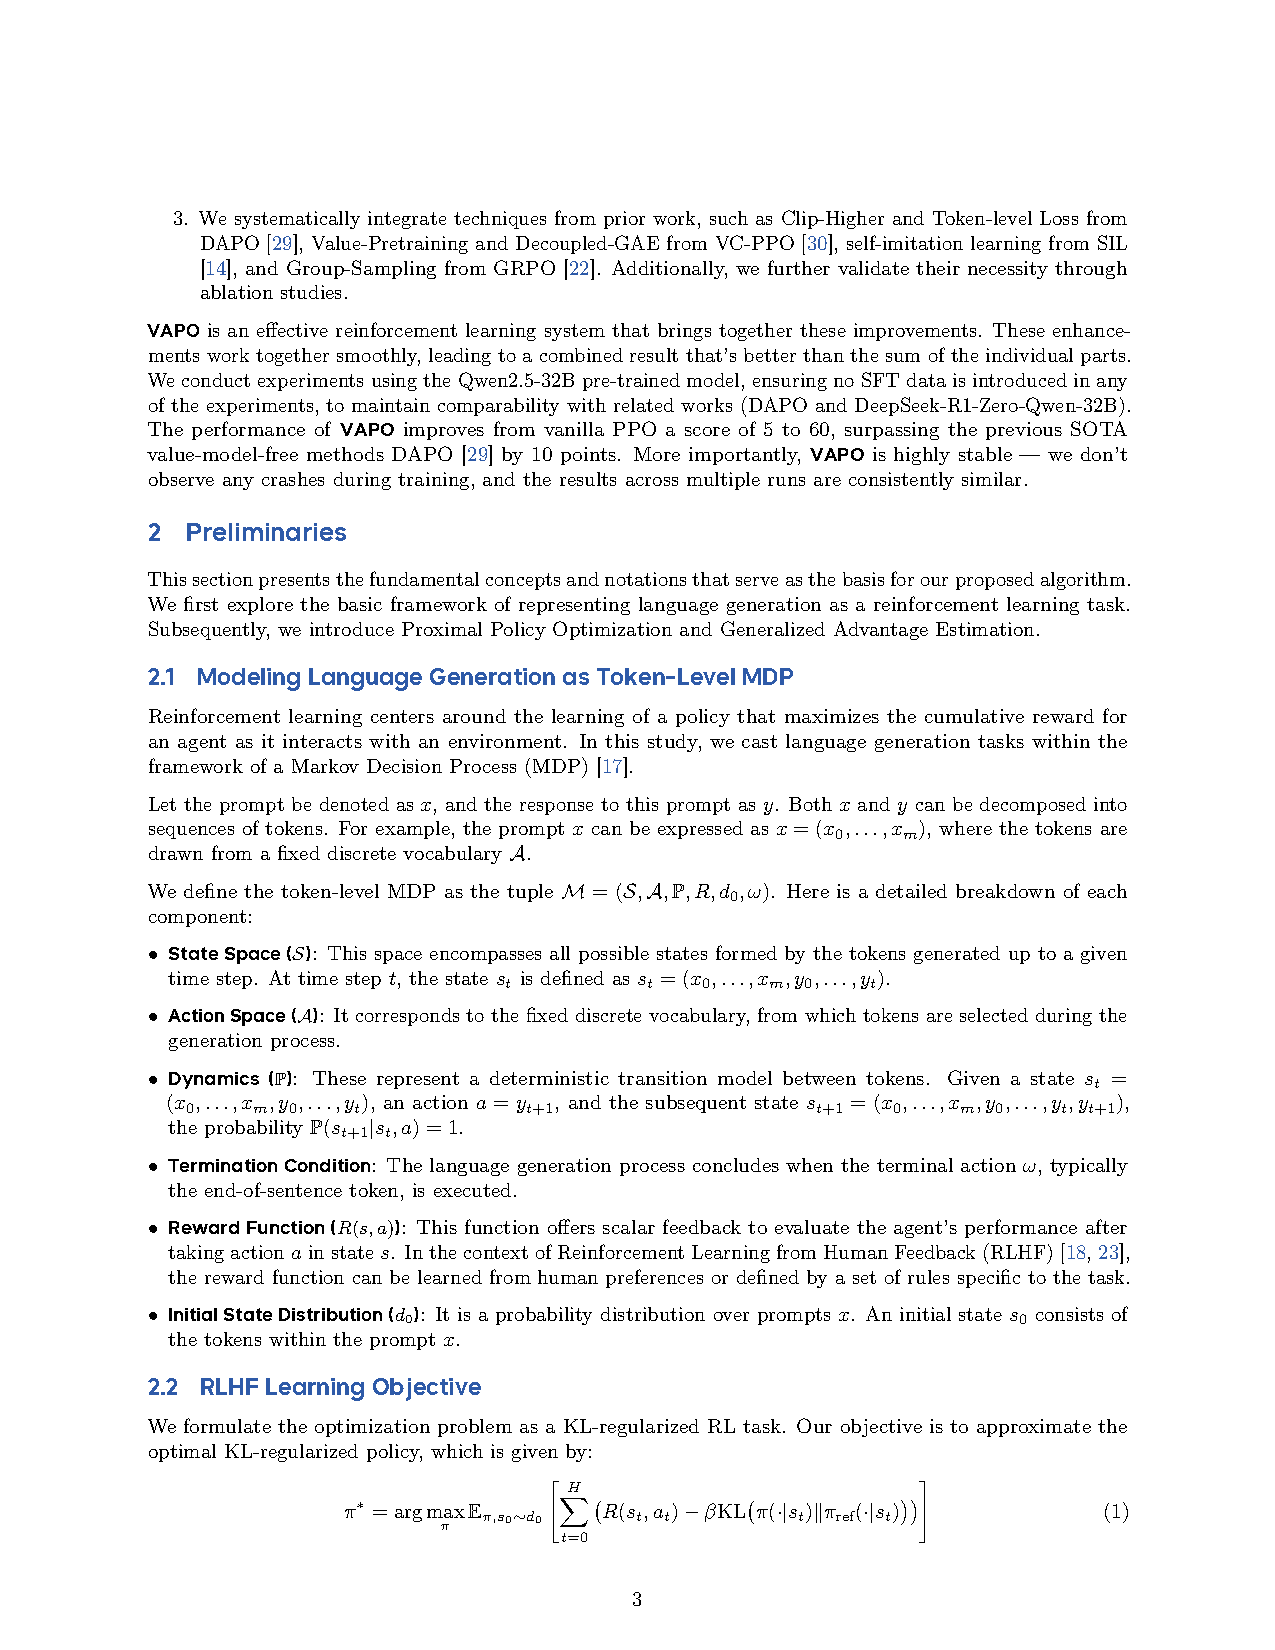
\includegraphics[width=\linewidth]{appendix_cases/case2/case2a.pdf}
        \subcaption{الجزء الأول من ملف PDF الإنجليزي للحالة 1.}
        \label{fig:source1}
    \end{subfigure}
    \hfill
    \begin{subfigure}[t]{0.48\textwidth}
        \centering
        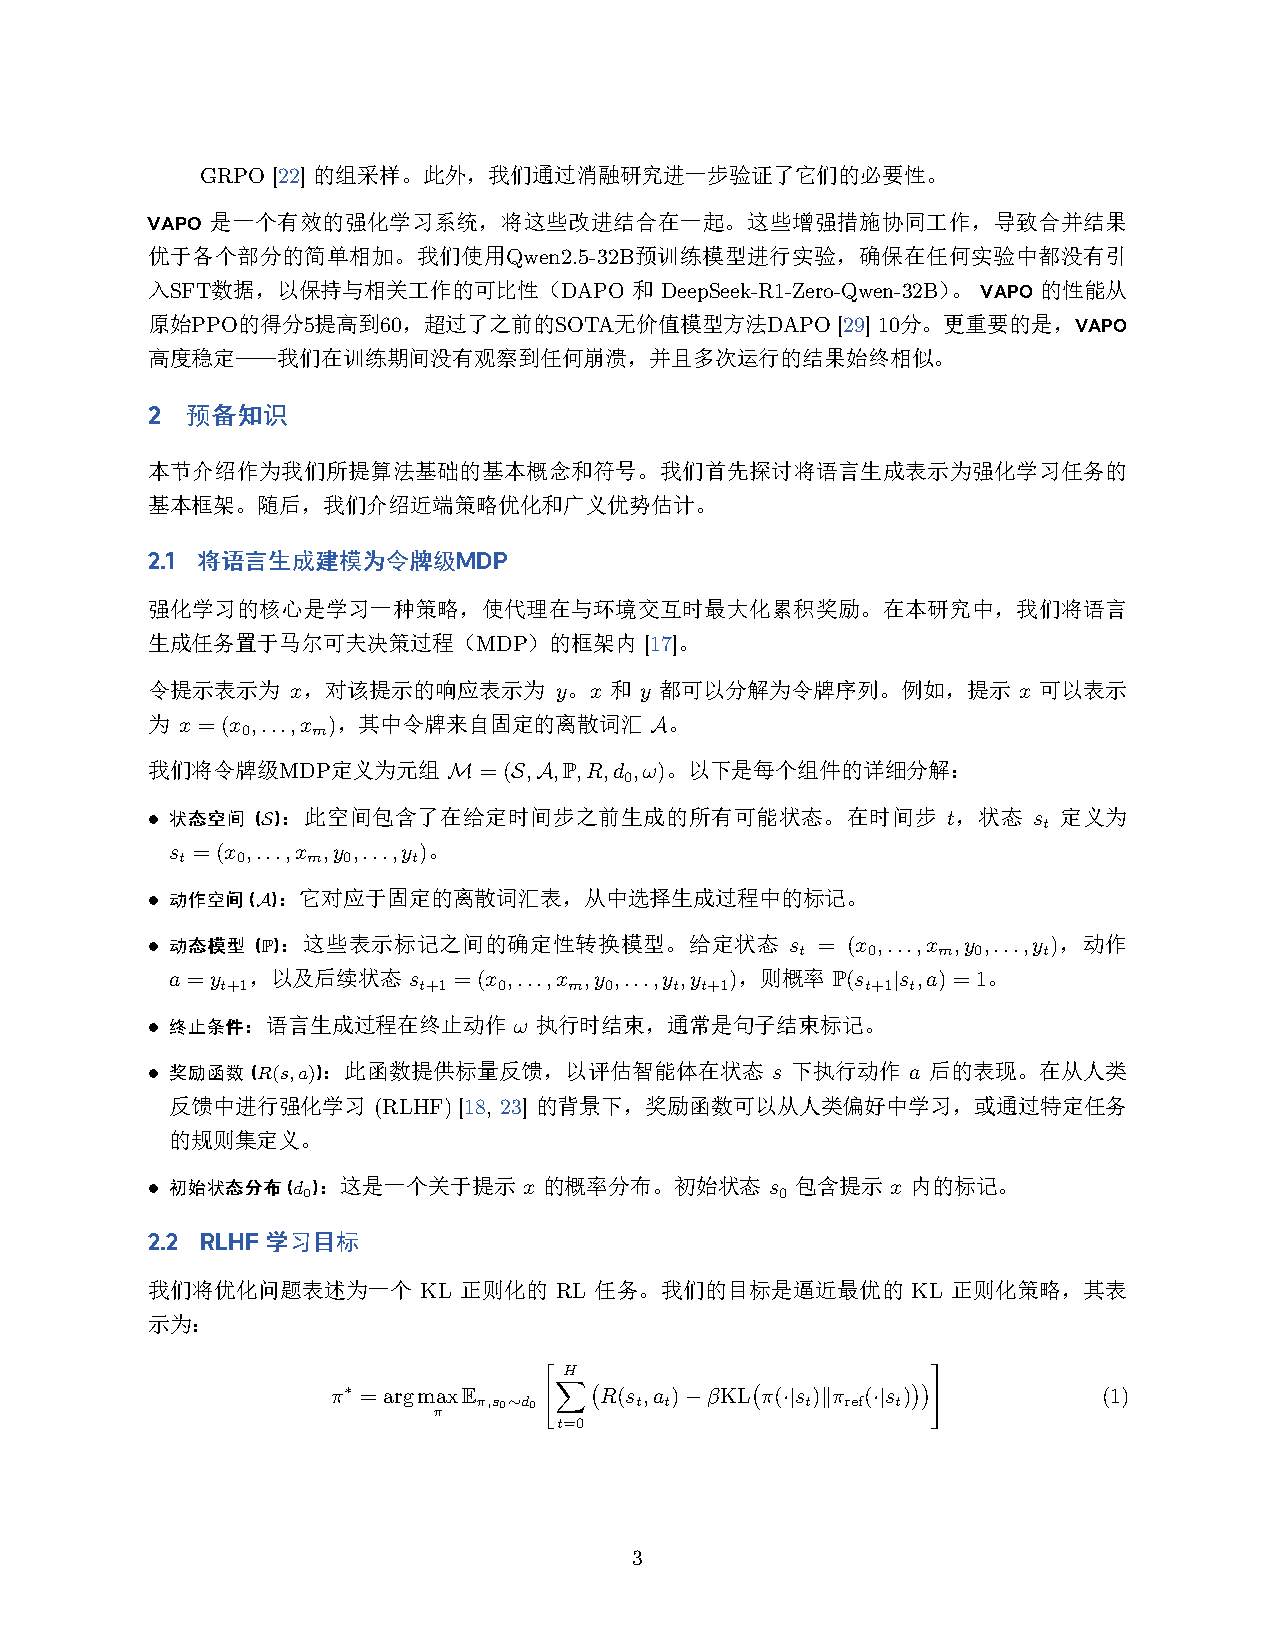
\includegraphics[width=\linewidth]{appendix_cases/case2/case2b.pdf}
        \subcaption{الجزء الأول من ملف PDF الصيني للحالة 1.}
        \label{fig:trans1}
    \end{subfigure}

    \begin{subfigure}[t]{0.48\textwidth}
        \centering
        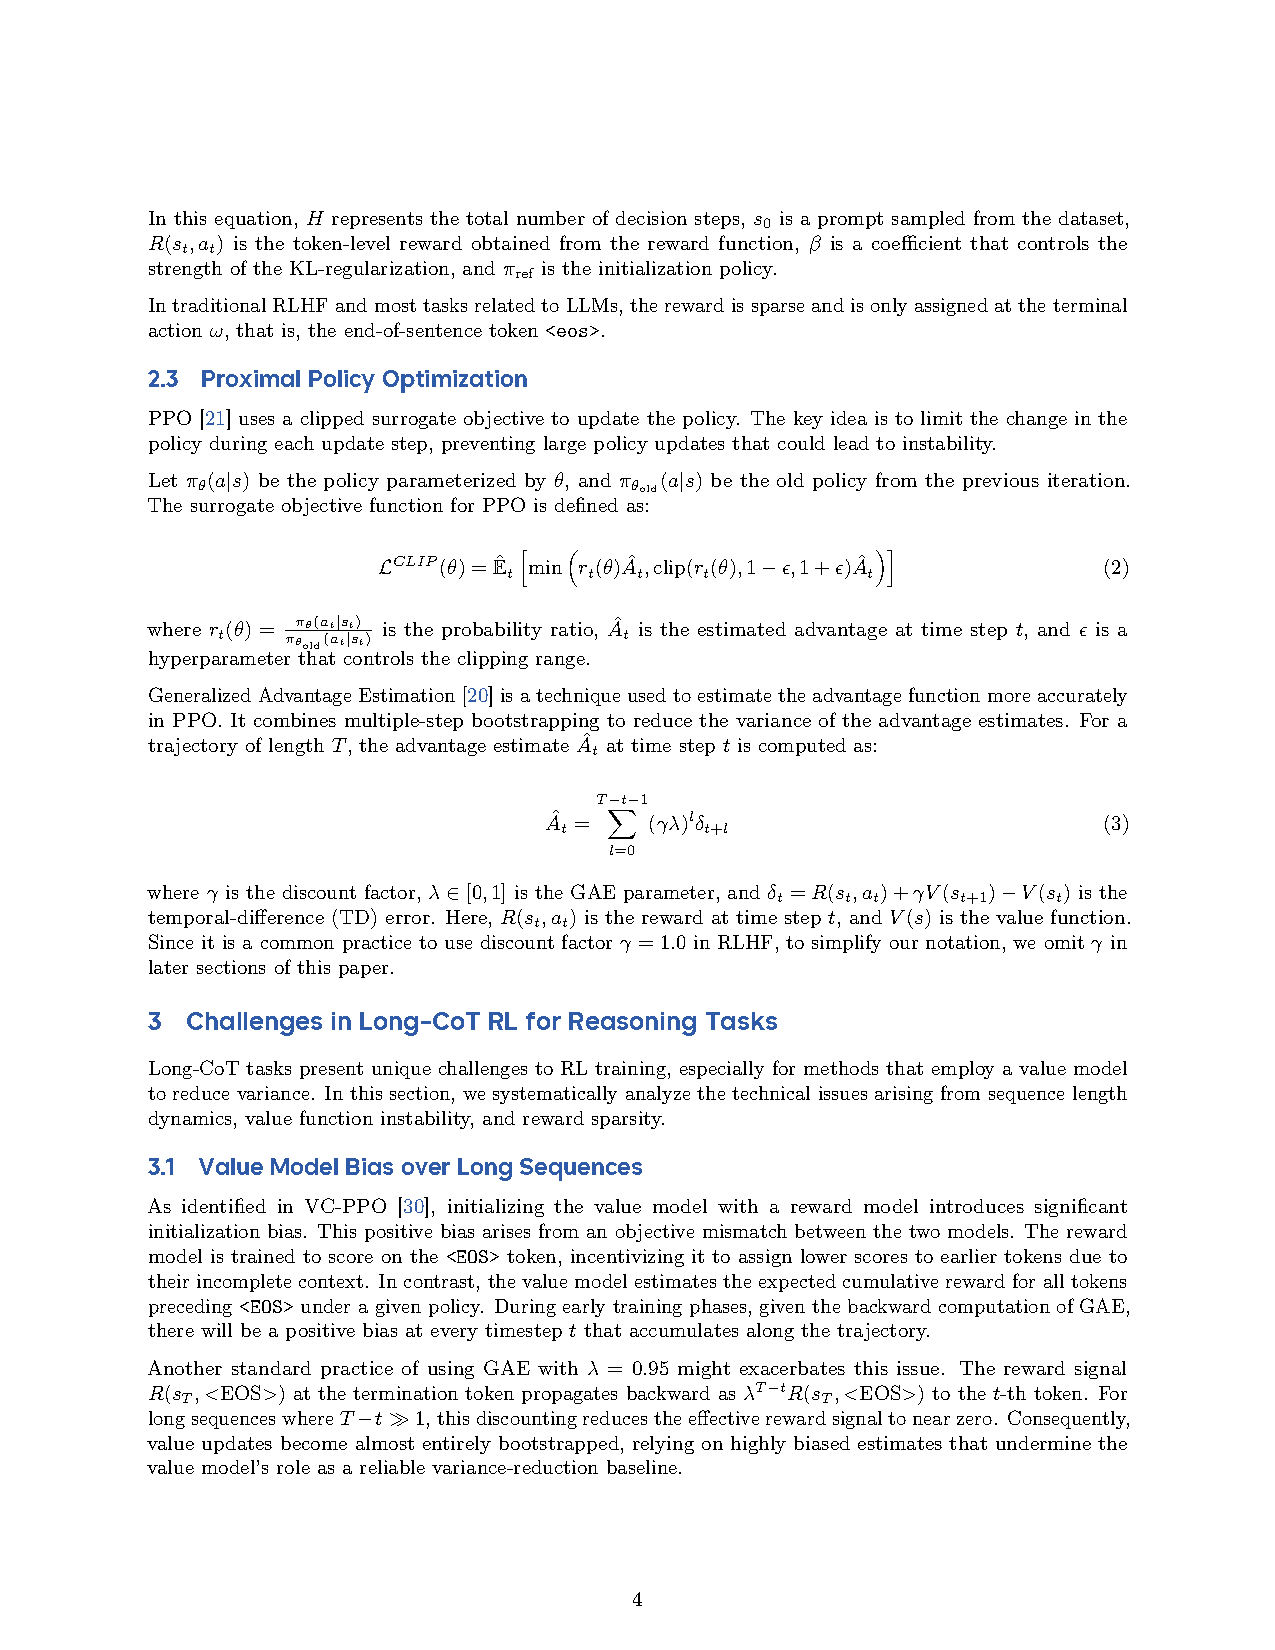
\includegraphics[width=\linewidth]{appendix_cases/case2/case2c}
        \subcaption{الجزء الثاني من ملف PDF باللغة الإنجليزية للحالة 1.}
    \end{subfigure}
    \hfill
    \begin{subfigure}[t]{0.48\textwidth}
        \centering
        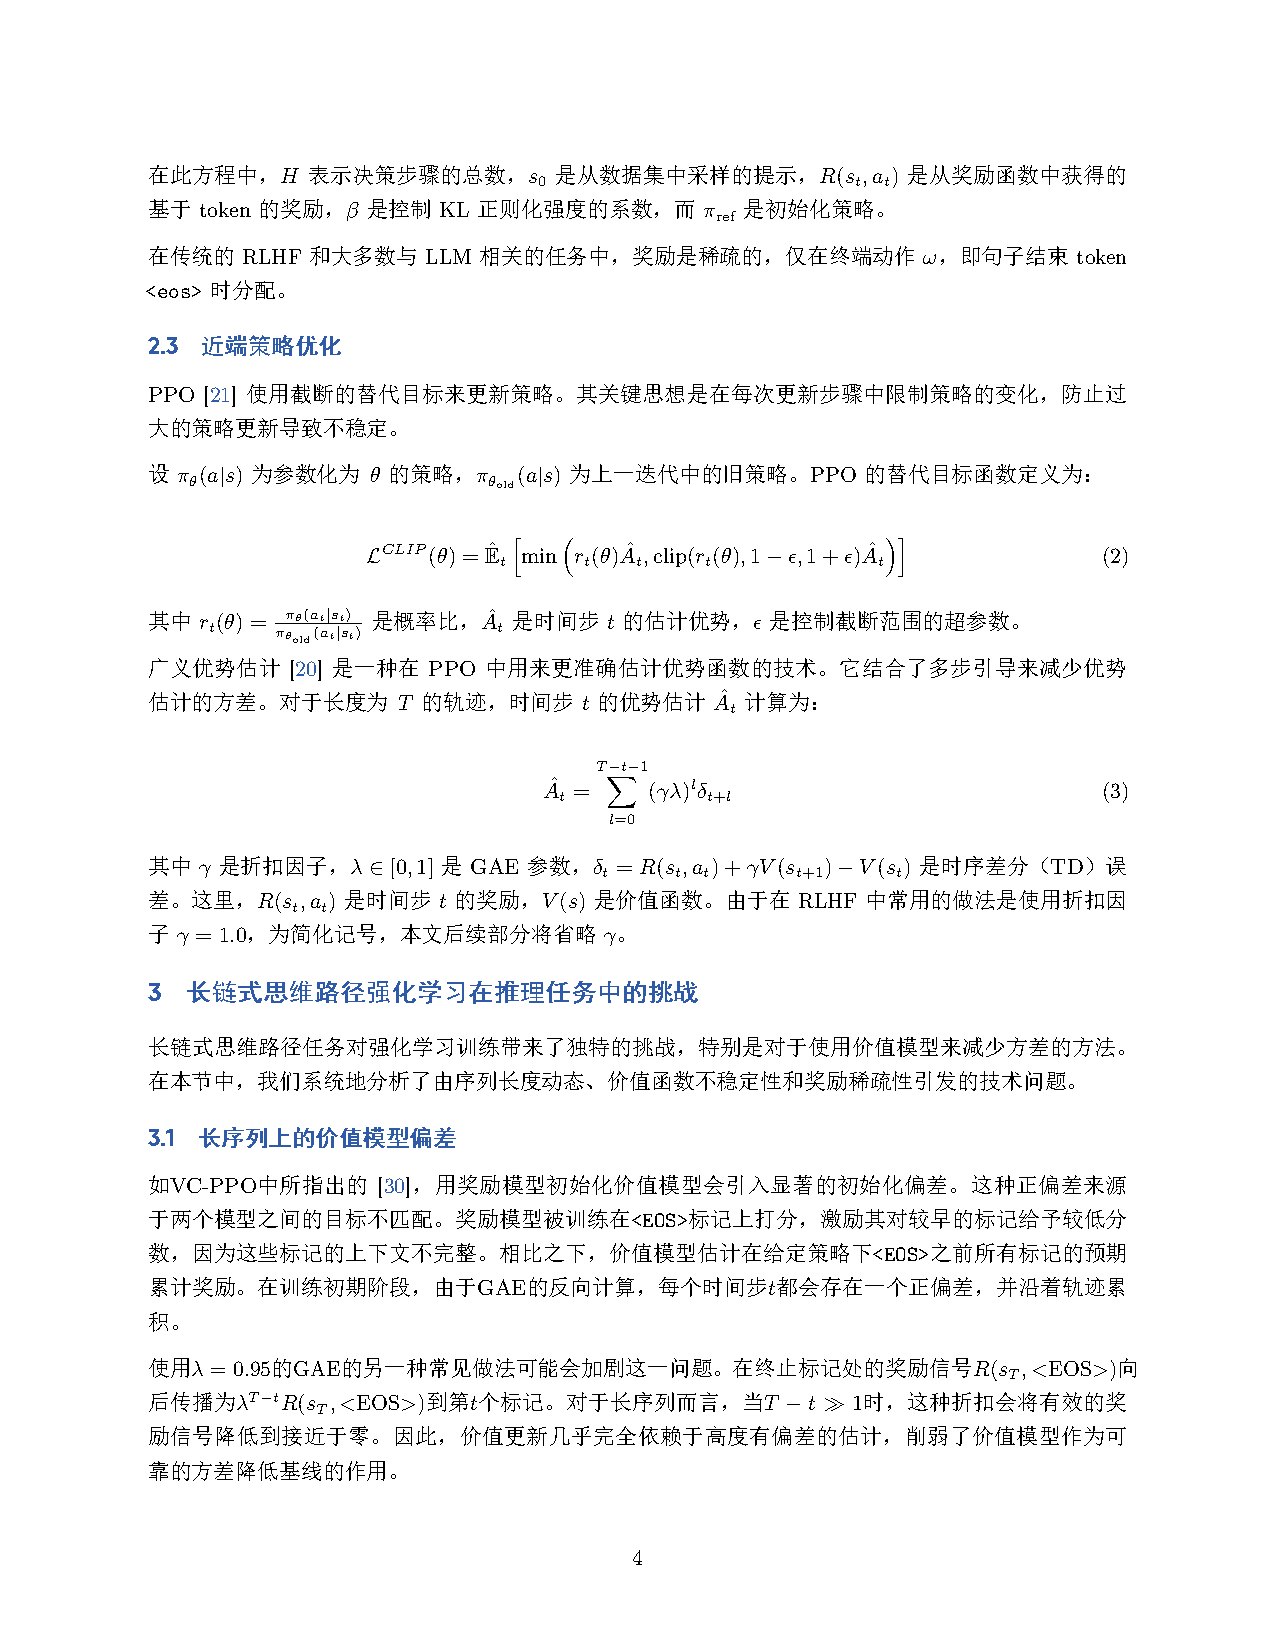
\includegraphics[width=\linewidth]{appendix_cases/case2/case2d.pdf}
        \subcaption{الجزء الثاني من ملف PDF الصيني للحالة 1.}
    \end{subfigure}

    \caption{الحالة 1 توضح أداء LaTeXTrans في مهمة En-Zh}
    \label{fig:case1}
\end{figure*}
\begin{figure*}[htbp]
    \centering

    \begin{subfigure}[t]{0.48\textwidth}
        \centering
        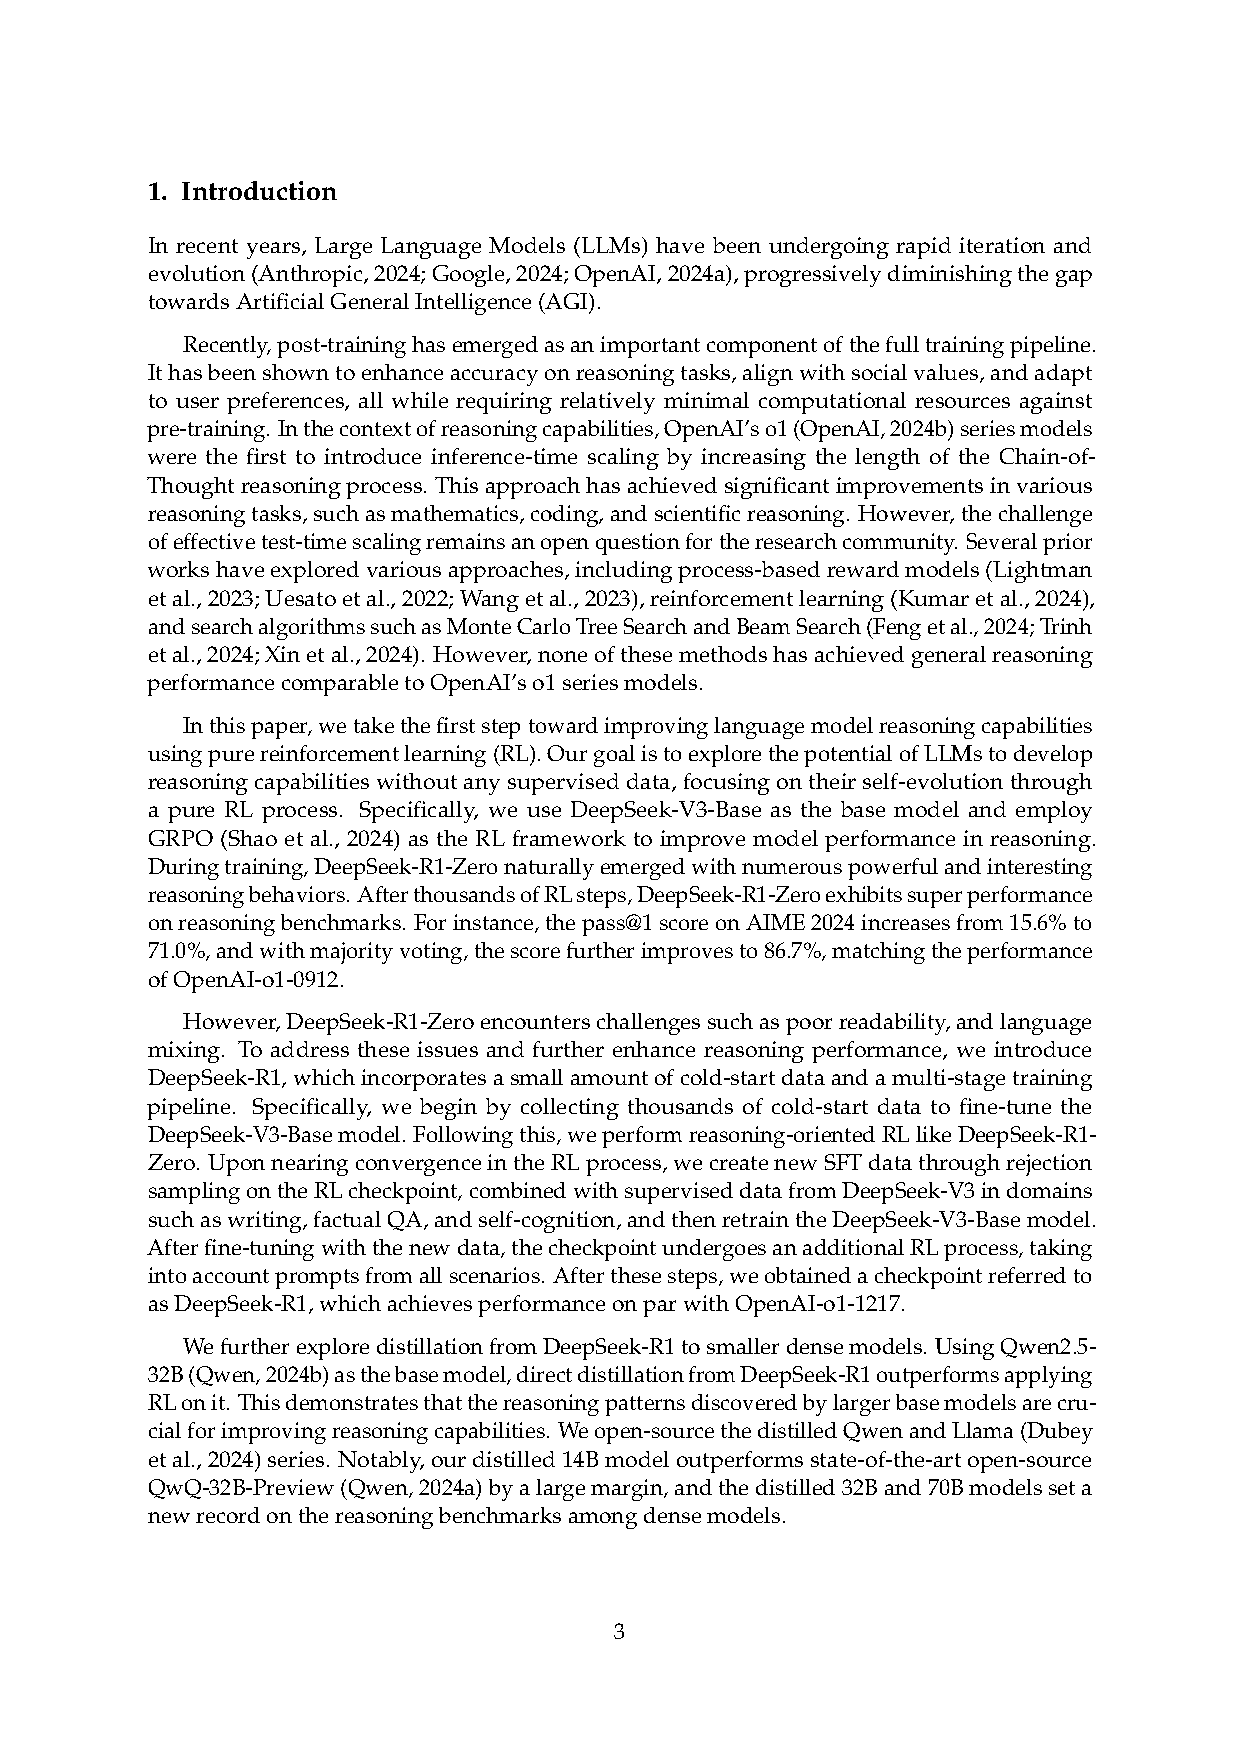
\includegraphics[width=\linewidth]{appendix_cases/case1/case1a}
        \subcaption{الجزء الأول من ملف PDF الإنجليزي للحالة 2.}
        \label{fig:source2}
    \end{subfigure}
    \hfill
    \begin{subfigure}[t]{0.48\textwidth}
        \centering
        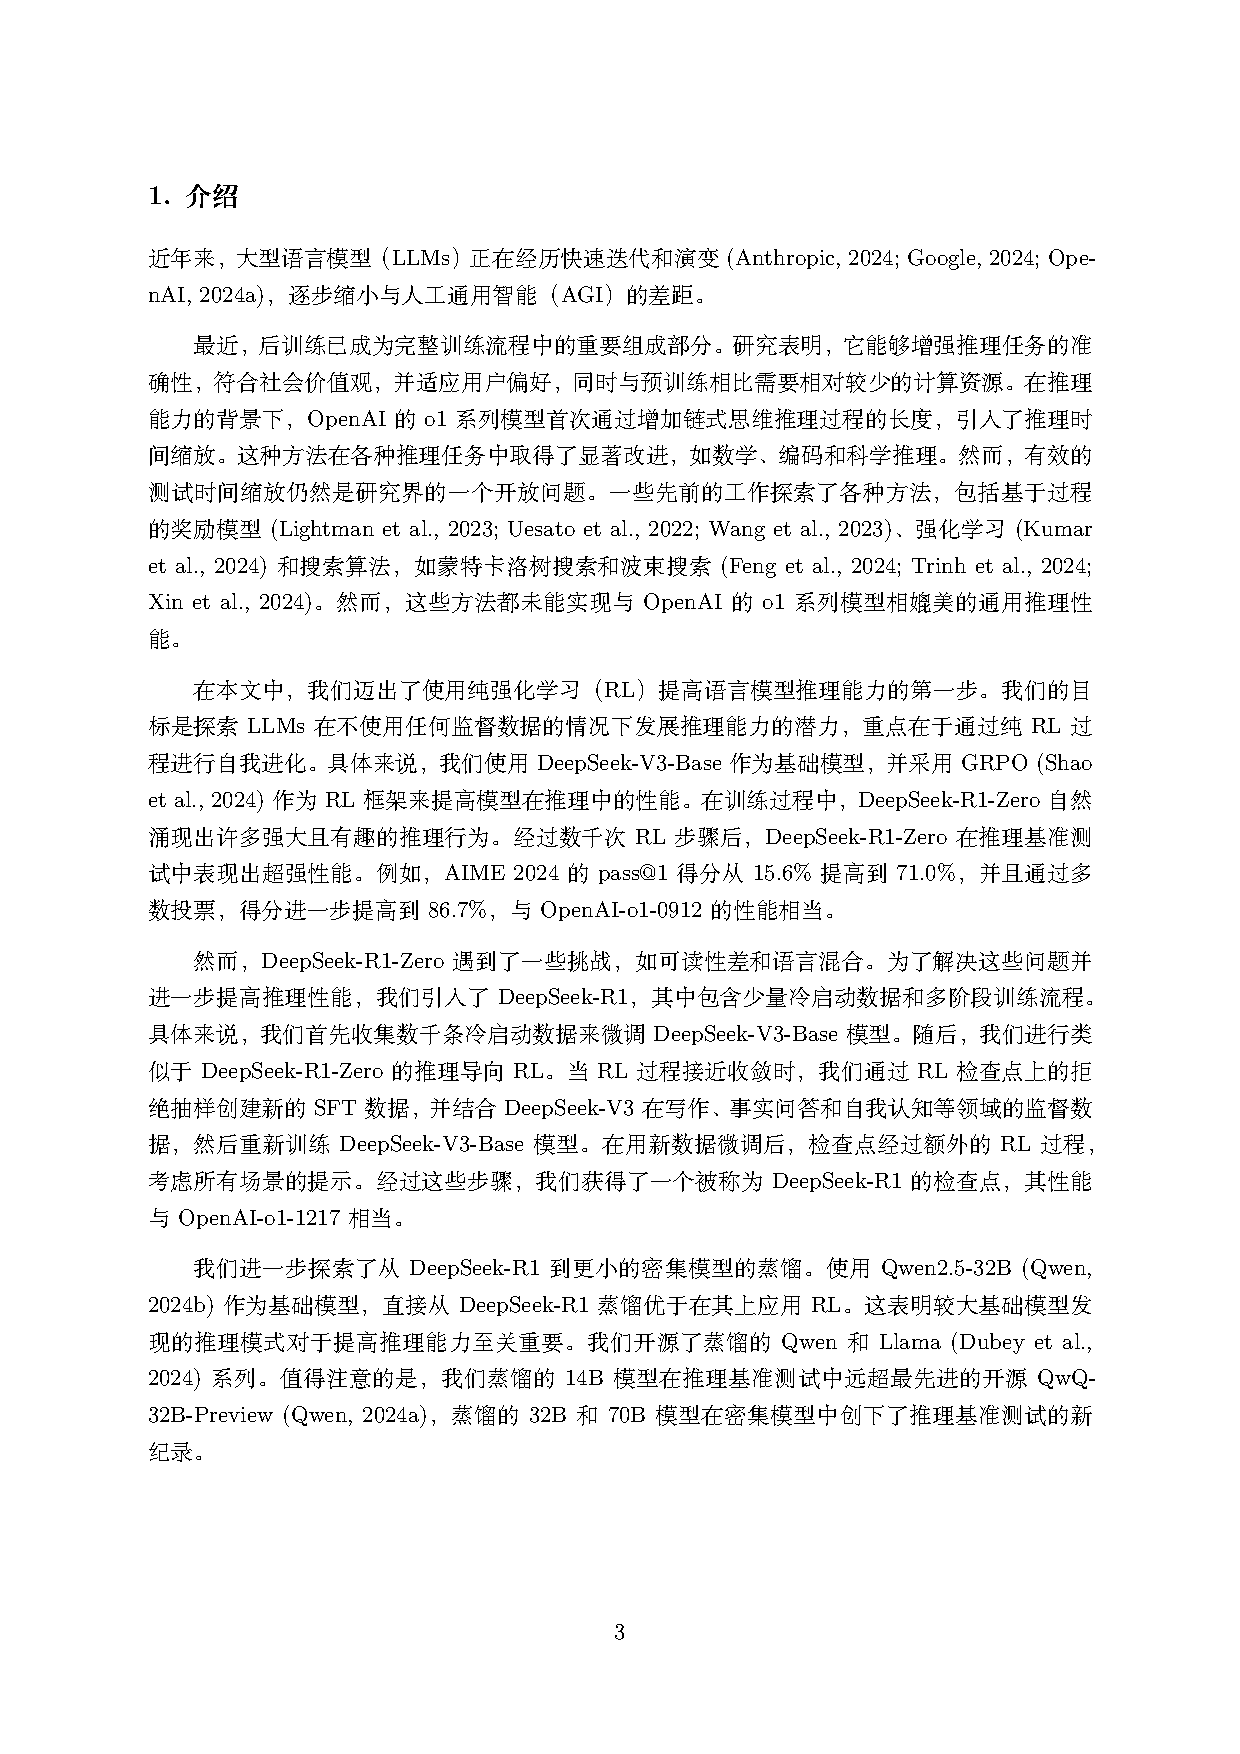
\includegraphics[width=\linewidth]{appendix_cases/case1/case1b}
        \subcaption{الجزء الأول من ملف PDF الصيني للحالة 2.}
        \label{fig:trans2}
    \end{subfigure}

    \begin{subfigure}[t]{0.48\textwidth}
        \centering
        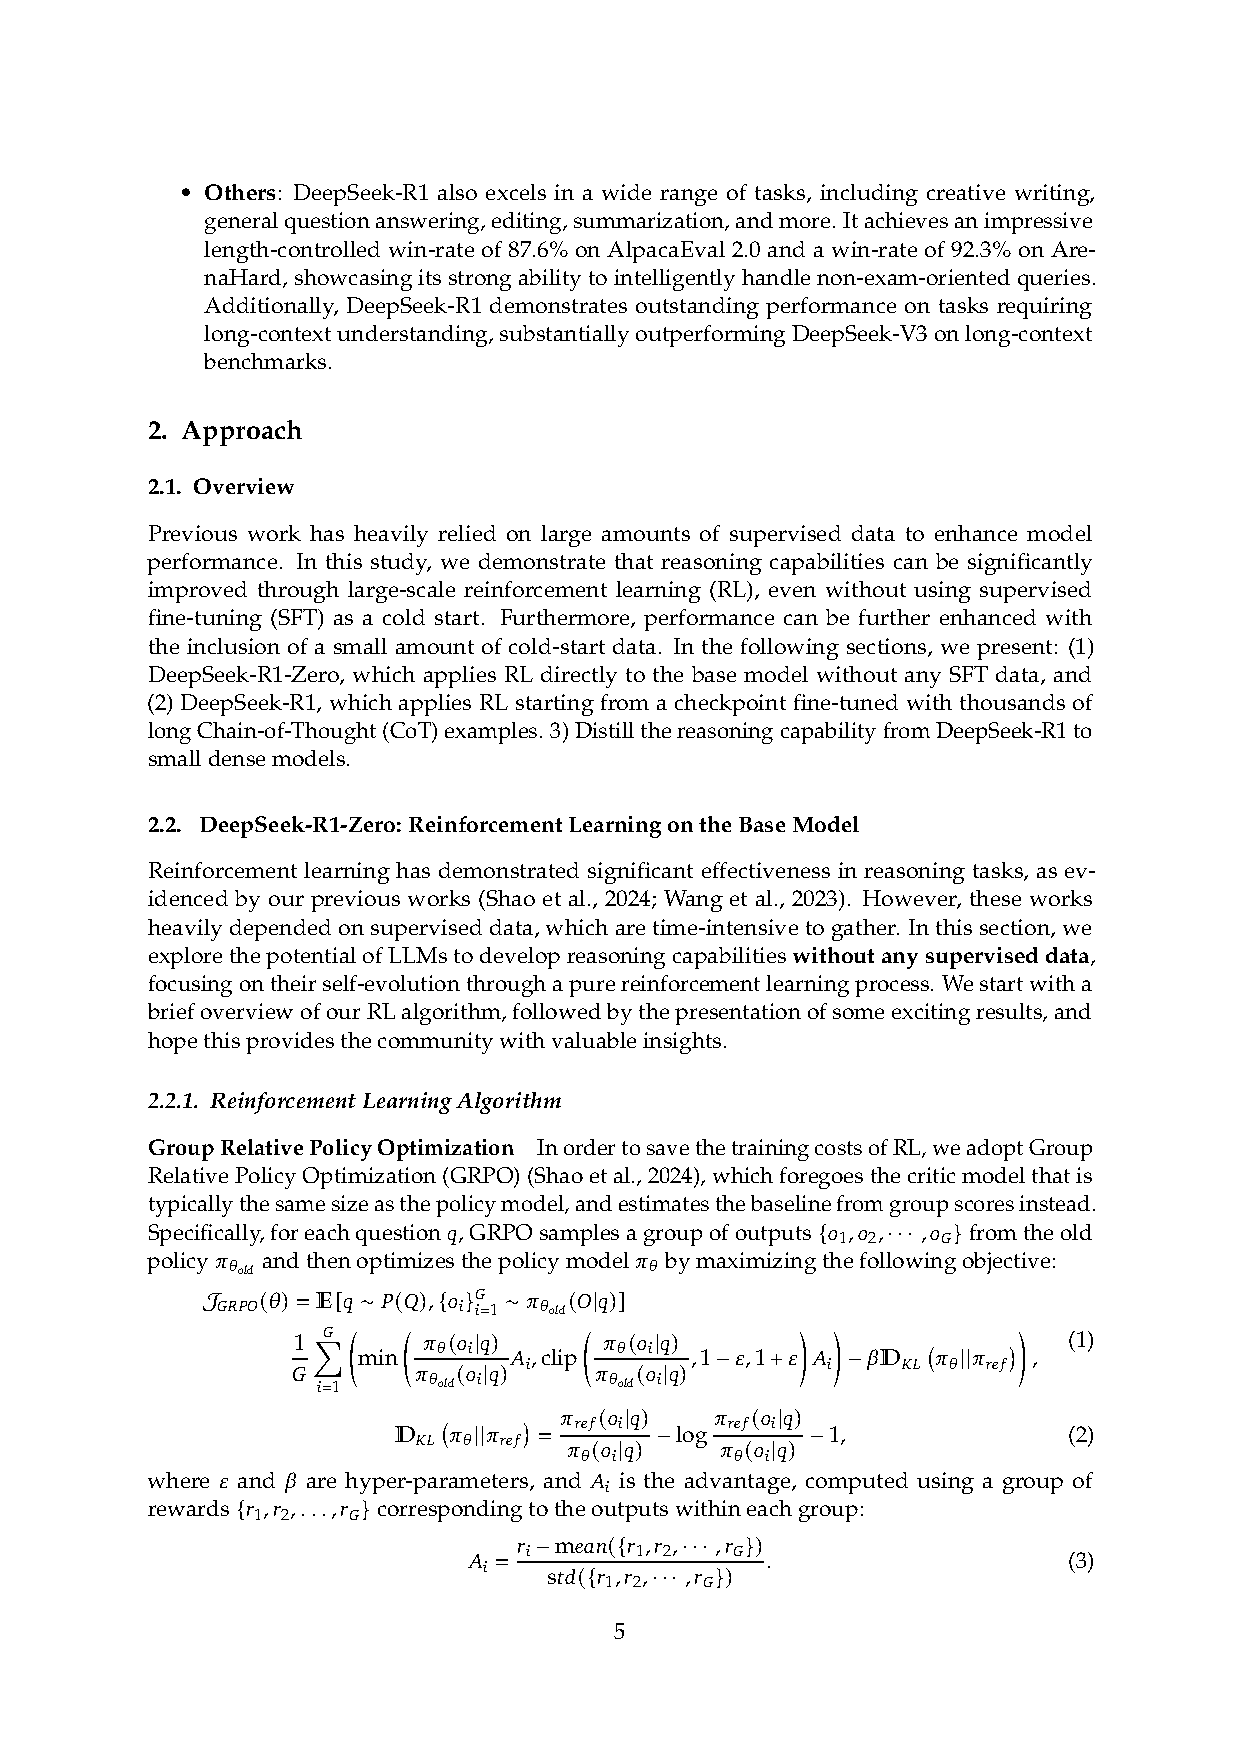
\includegraphics[width=\linewidth]{appendix_cases/case1/case1c}
        \subcaption{الجزء الثاني من ملف PDF باللغة الإنجليزية للحالة 2.}
    \end{subfigure}
    \hfill
    \begin{subfigure}[t]{0.48\textwidth}
        \centering
        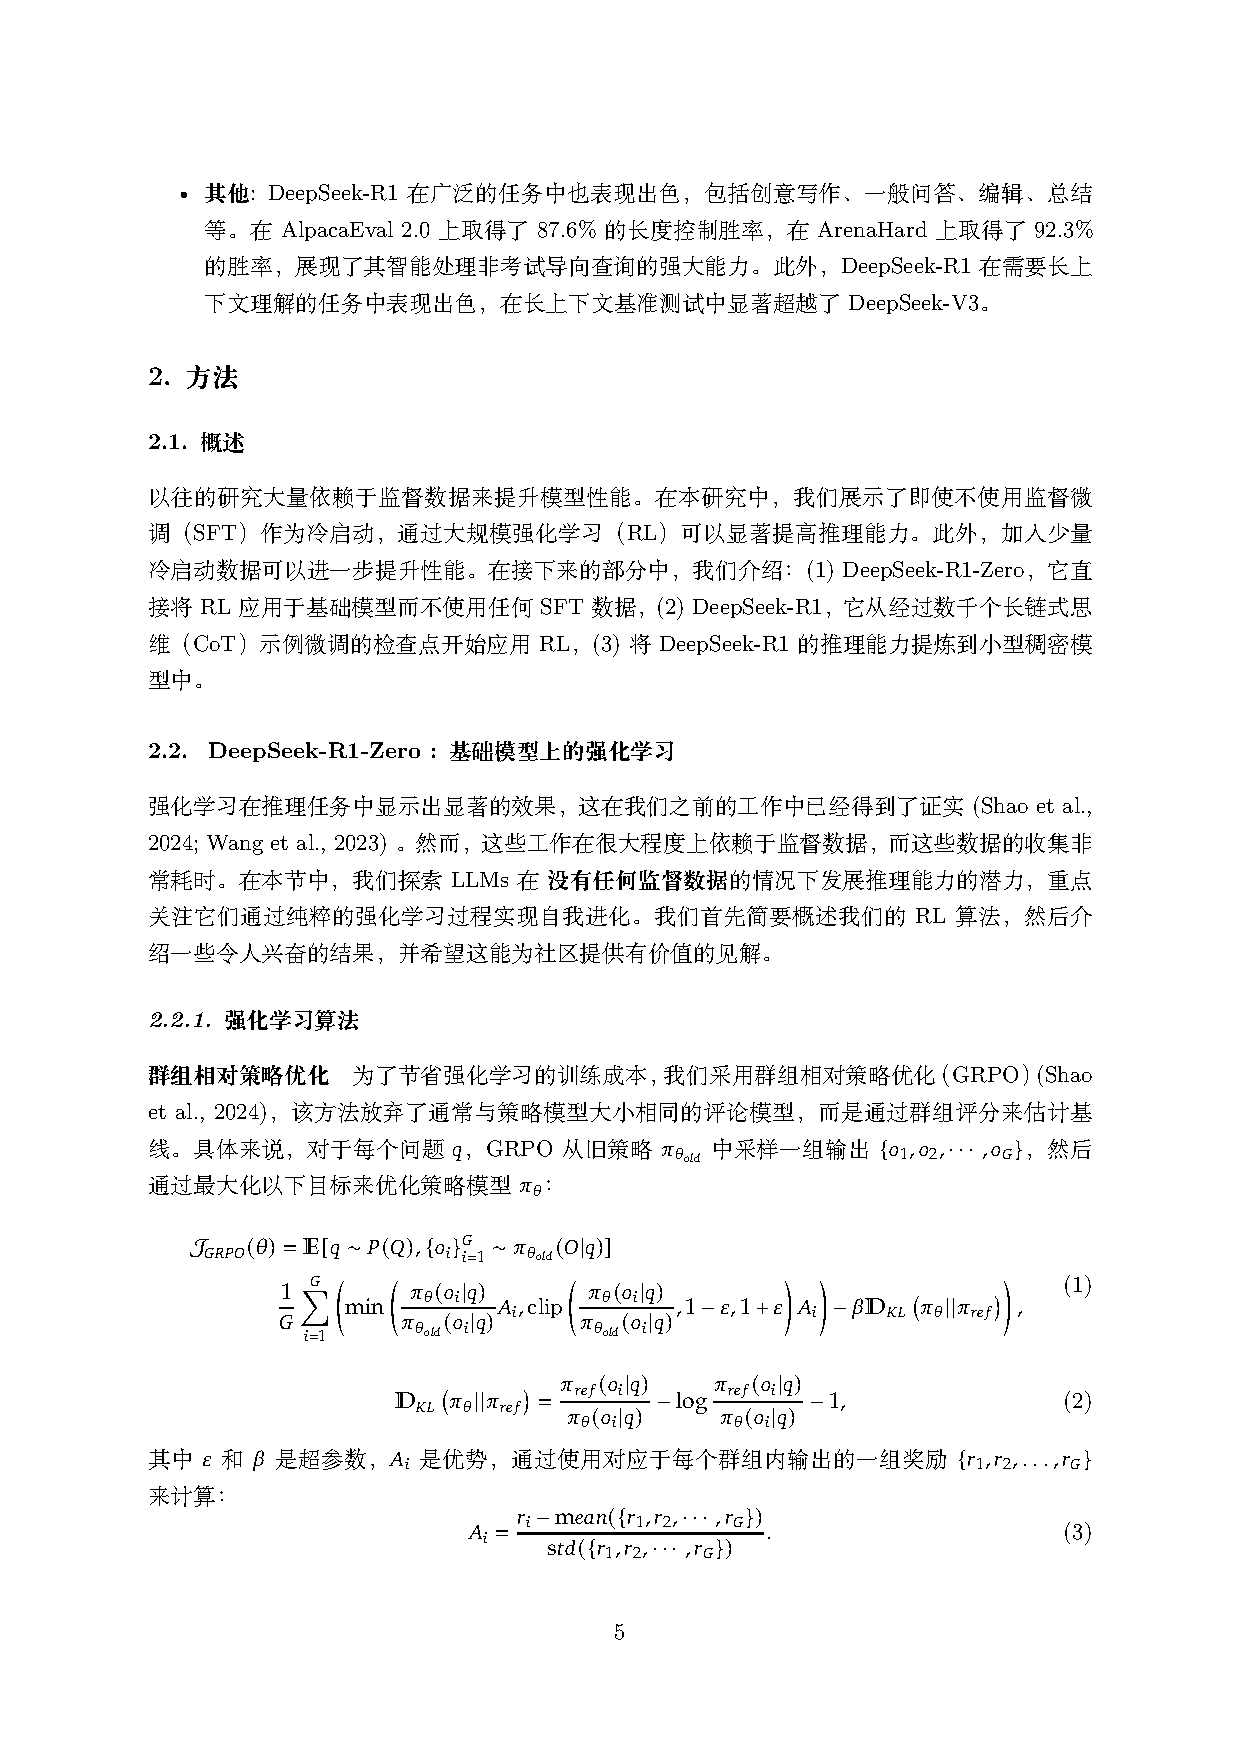
\includegraphics[width=\linewidth]{appendix_cases/case1/case1d}
        \subcaption{الجزء الثاني من ملف PDF الصيني للحالة 2.}
    \end{subfigure}

    \caption{الحالة 2 توضح أداء LaTeXTrans في مهمة En-Zh}
    \label{fig:case2}
\end{figure*}
\begin{figure*}[htbp]
    \centering

    \begin{subfigure}[t]{0.48\textwidth}
        \centering
        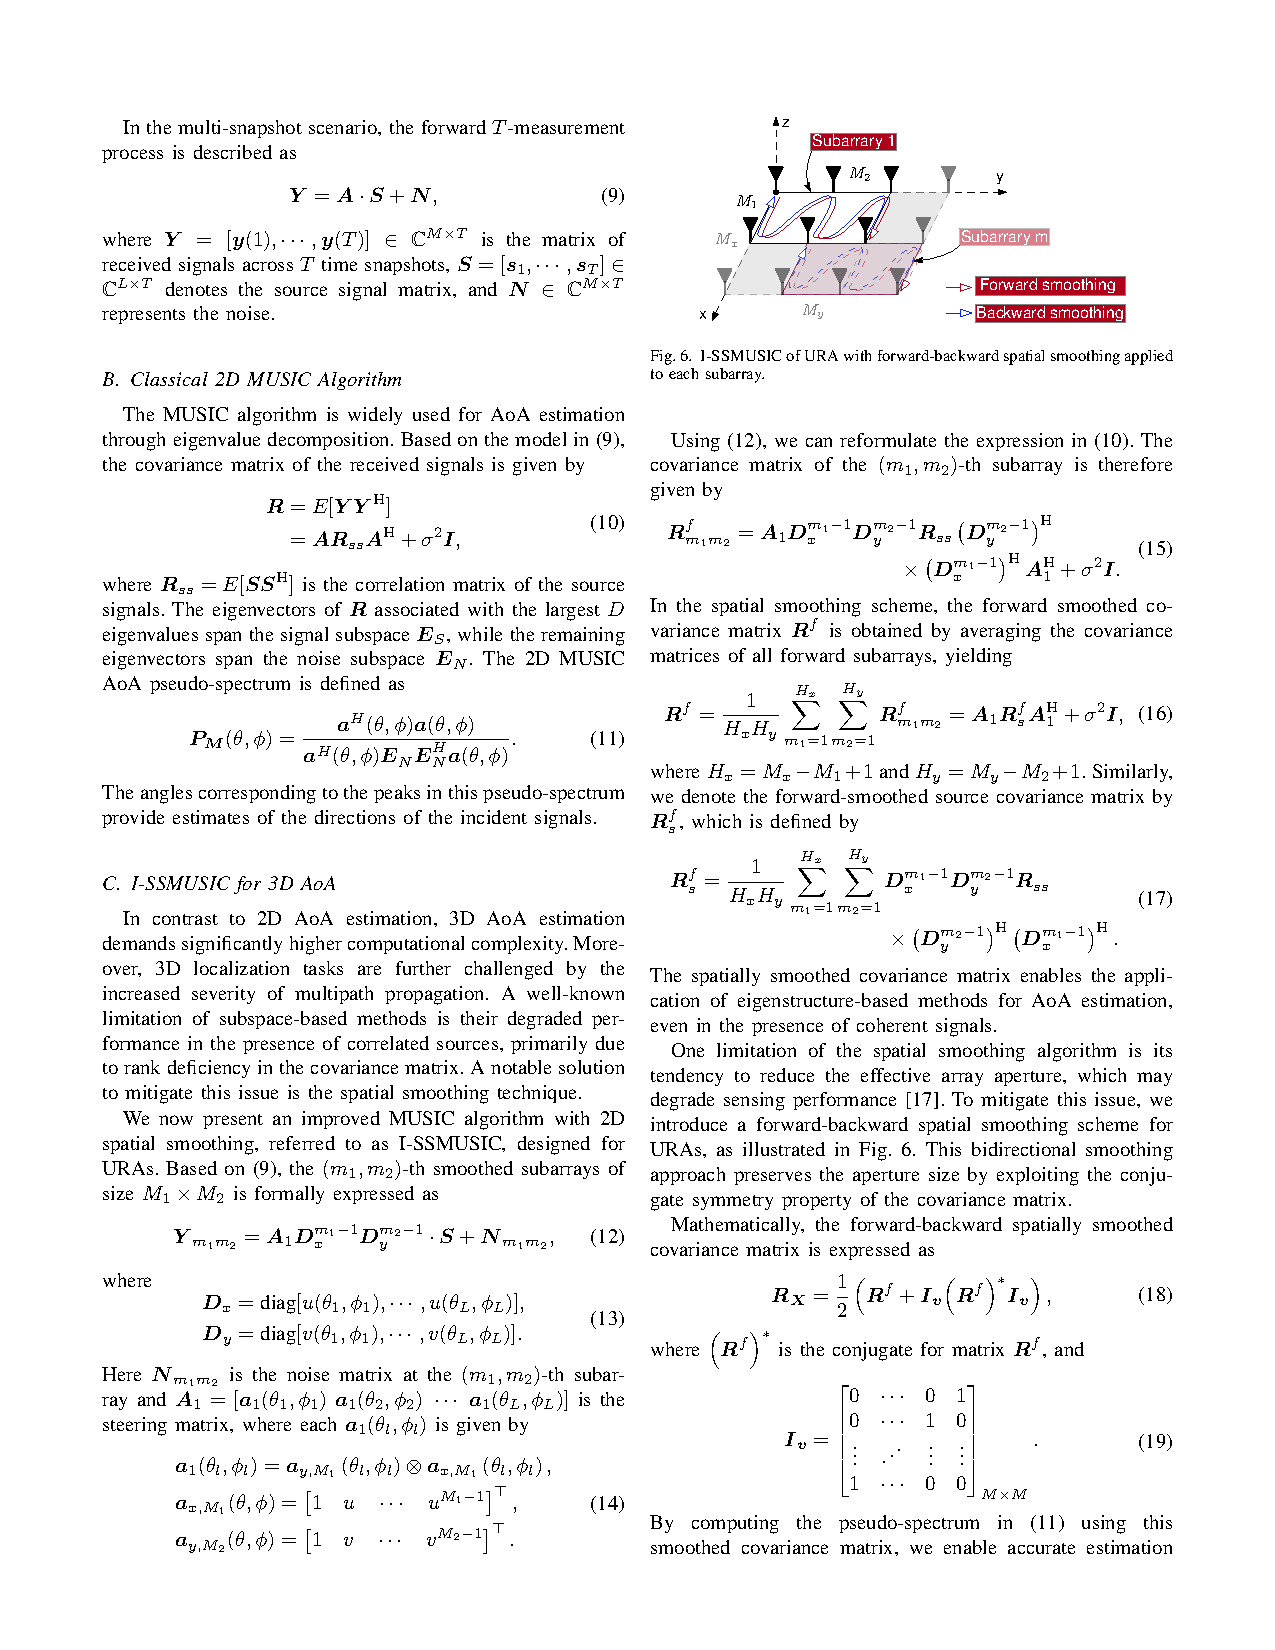
\includegraphics[width=\linewidth]{appendix_cases/case3/case3a}
        \subcaption{الجزء الأول من ملف PDF الإنجليزي للحالة 3.}
        \label{fig:source3}
    \end{subfigure}
    \hfill
    \begin{subfigure}[t]{0.48\textwidth}
        \centering
        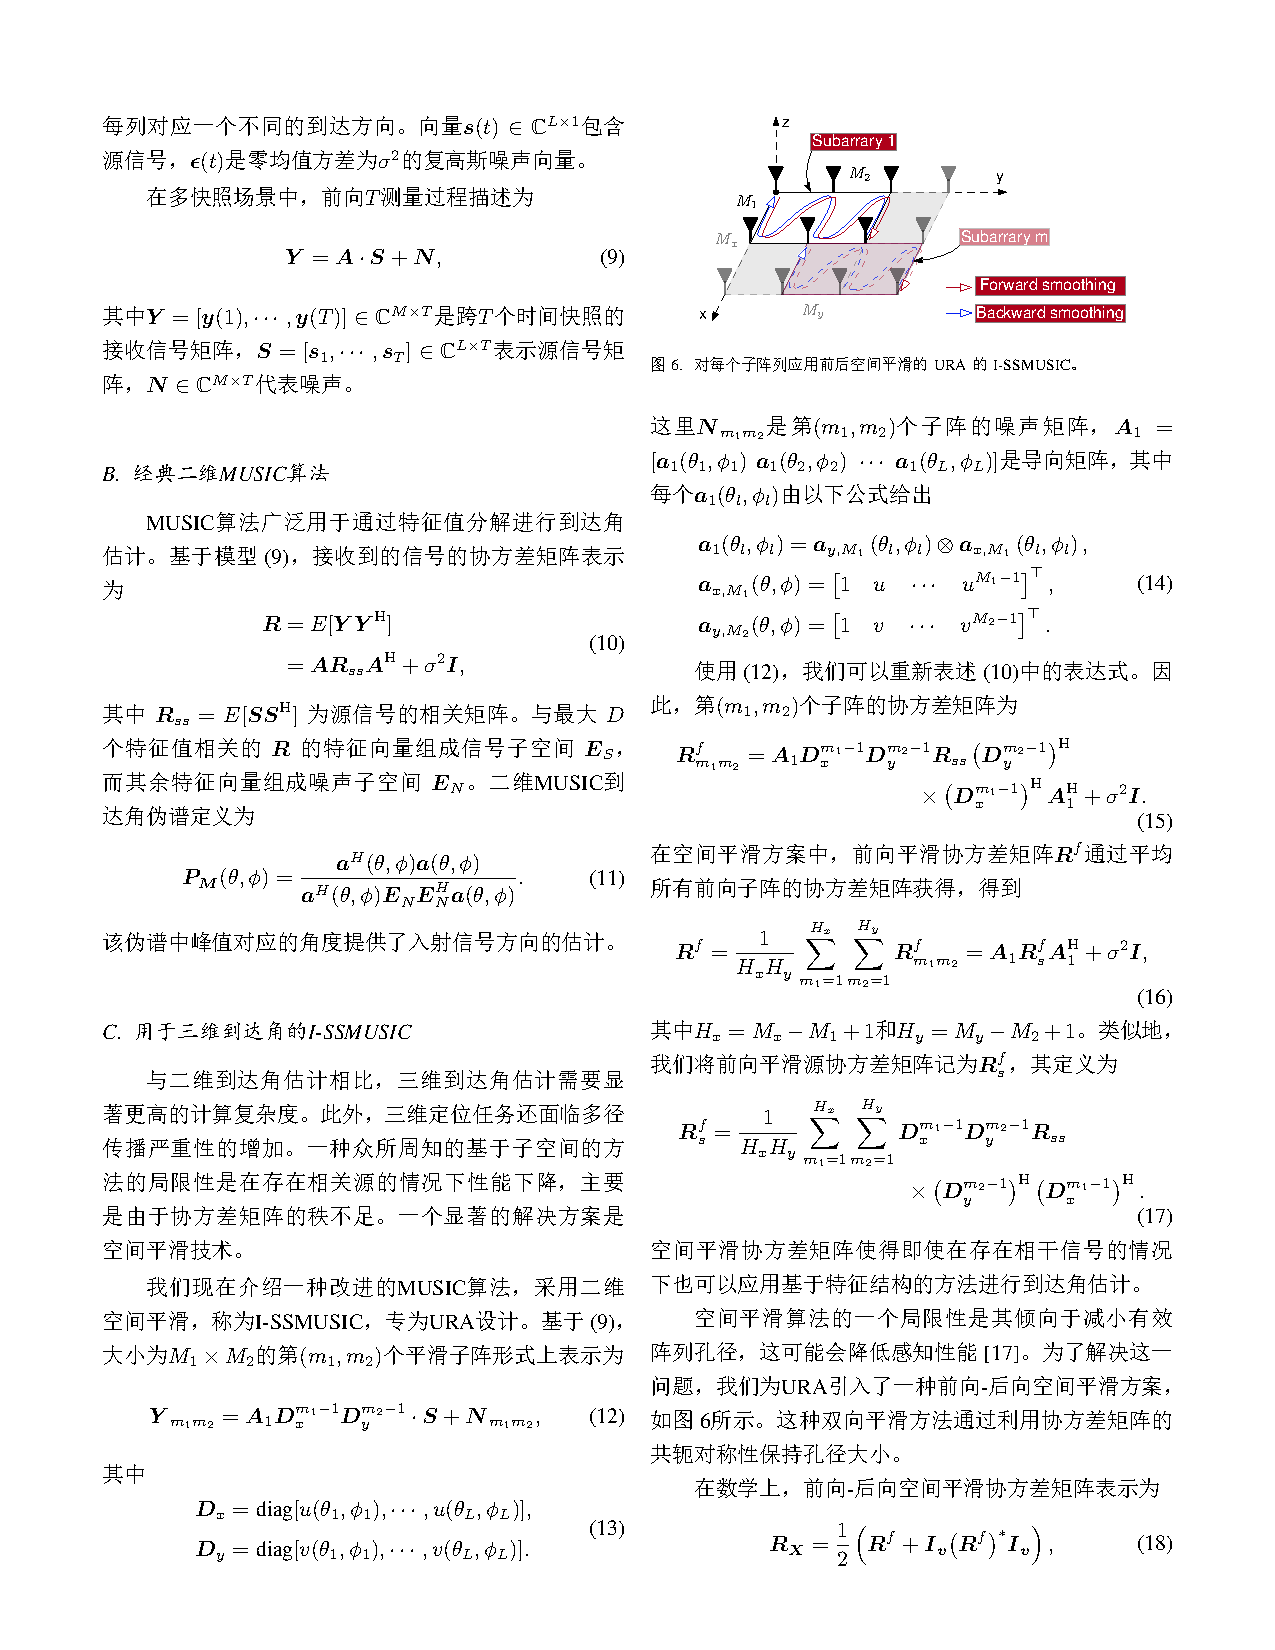
\includegraphics[width=\linewidth]{appendix_cases/case3/case3b}
        \subcaption{الجزء الأول من ملف PDF الصيني للحالة 3.}
        \label{fig:trans3}
    \end{subfigure}

    \begin{subfigure}[t]{0.48\textwidth}
        \centering
        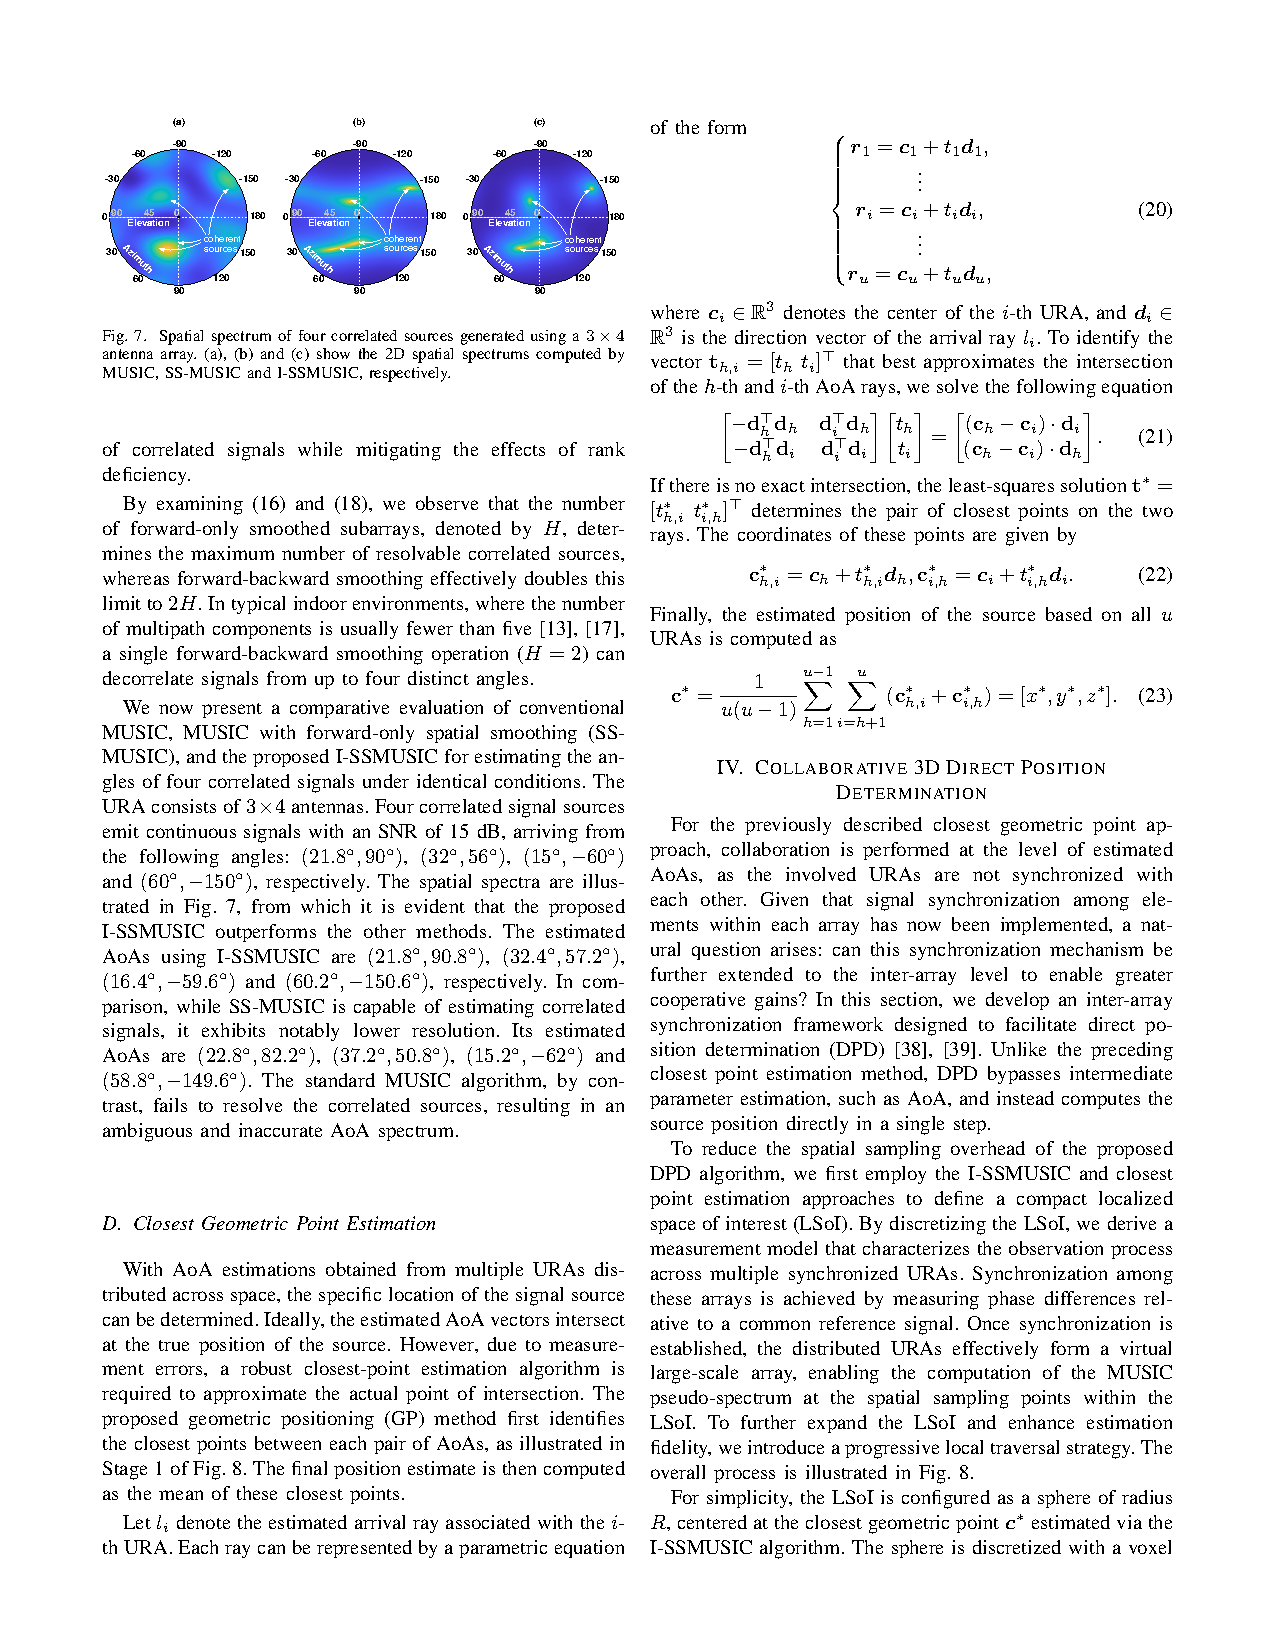
\includegraphics[width=\linewidth]{appendix_cases/case3/case3c}
        \subcaption{الجزء الثاني من ملف PDF الإنجليزي للحالة 3.}
    \end{subfigure}
    \hfill
    \begin{subfigure}[t]{0.48\textwidth}
        \centering
        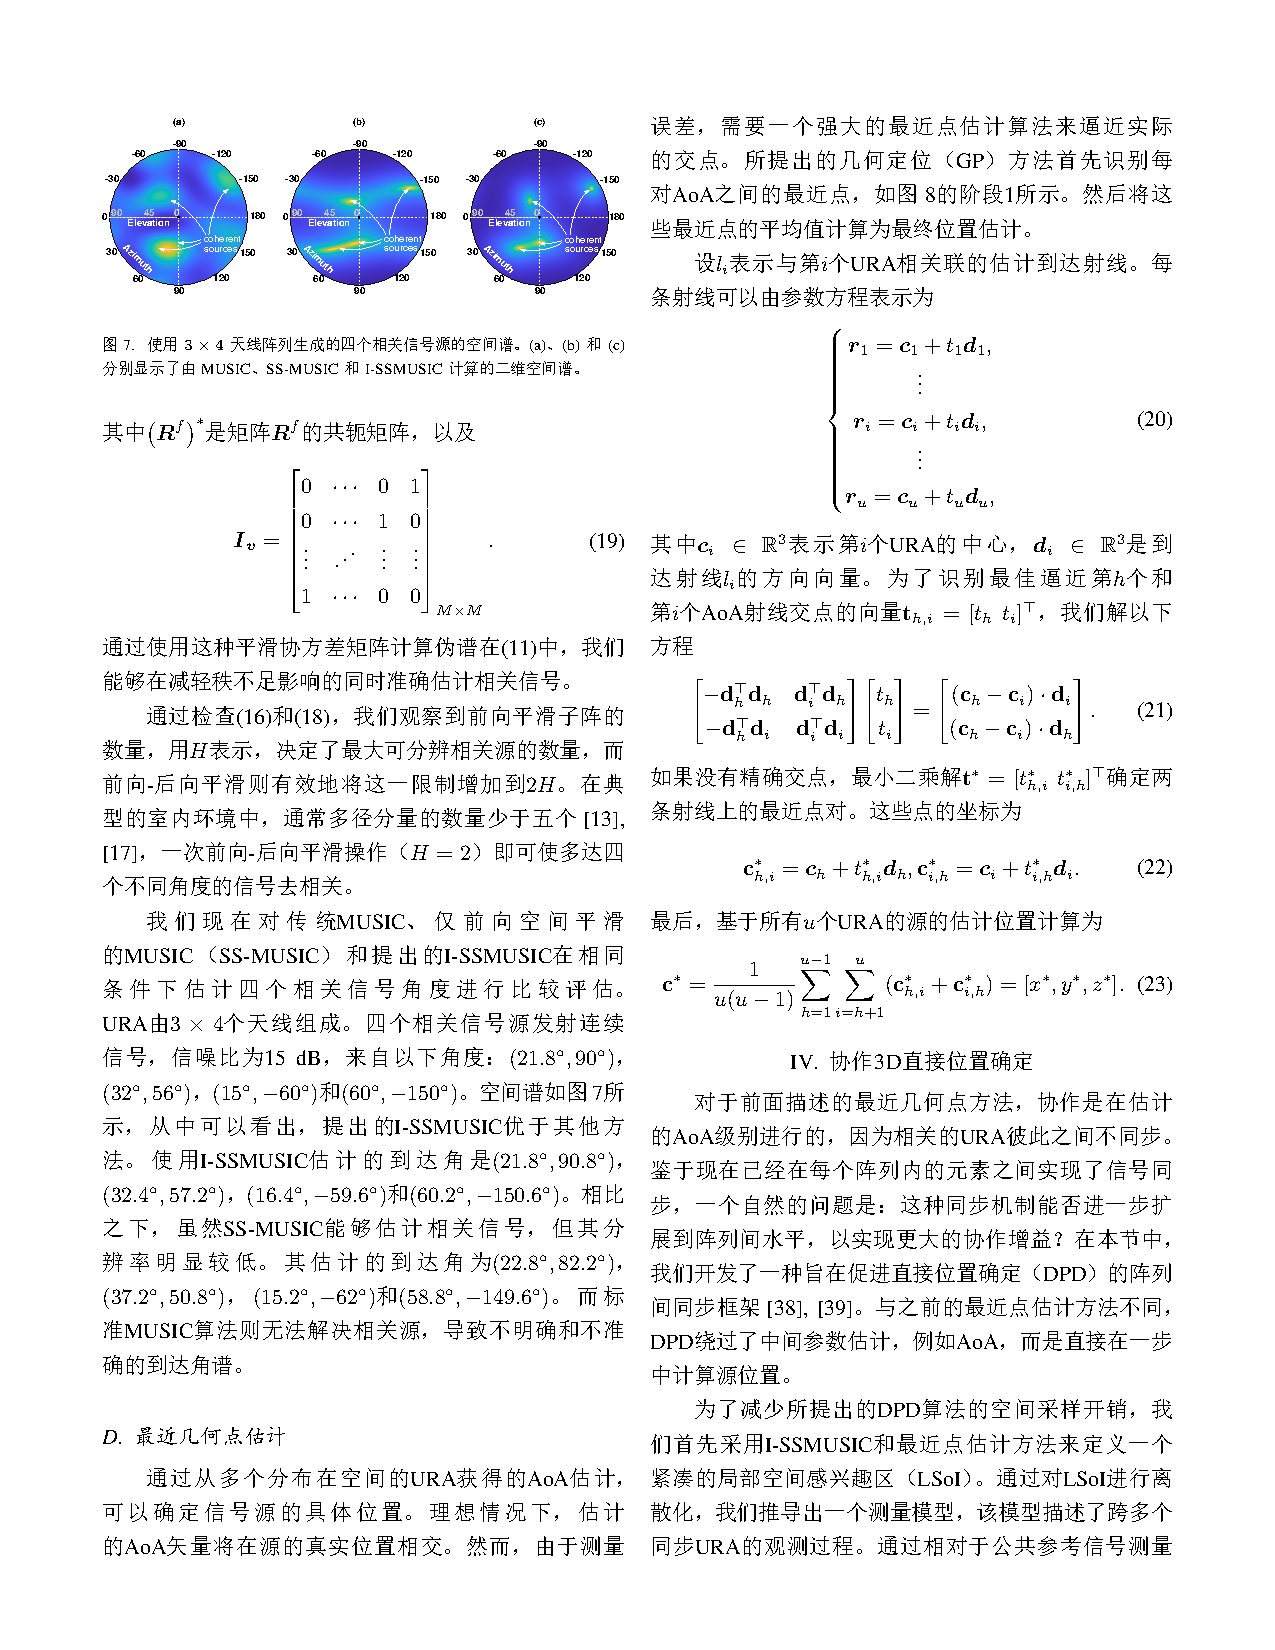
\includegraphics[width=\linewidth]{appendix_cases/case3/case3d}
        \subcaption{الجزء الثاني من ملف PDF الصيني للحالة 3.}
    \end{subfigure}

    \caption{تظهر الحالة 3 أداء LaTeXTrans في مهمة En-Zh}
    \label{fig:case3}
\end{figure*}

\begin{figure*}[htbp]
    \centering

    \begin{subfigure}[t]{0.48\textwidth}
        \centering
        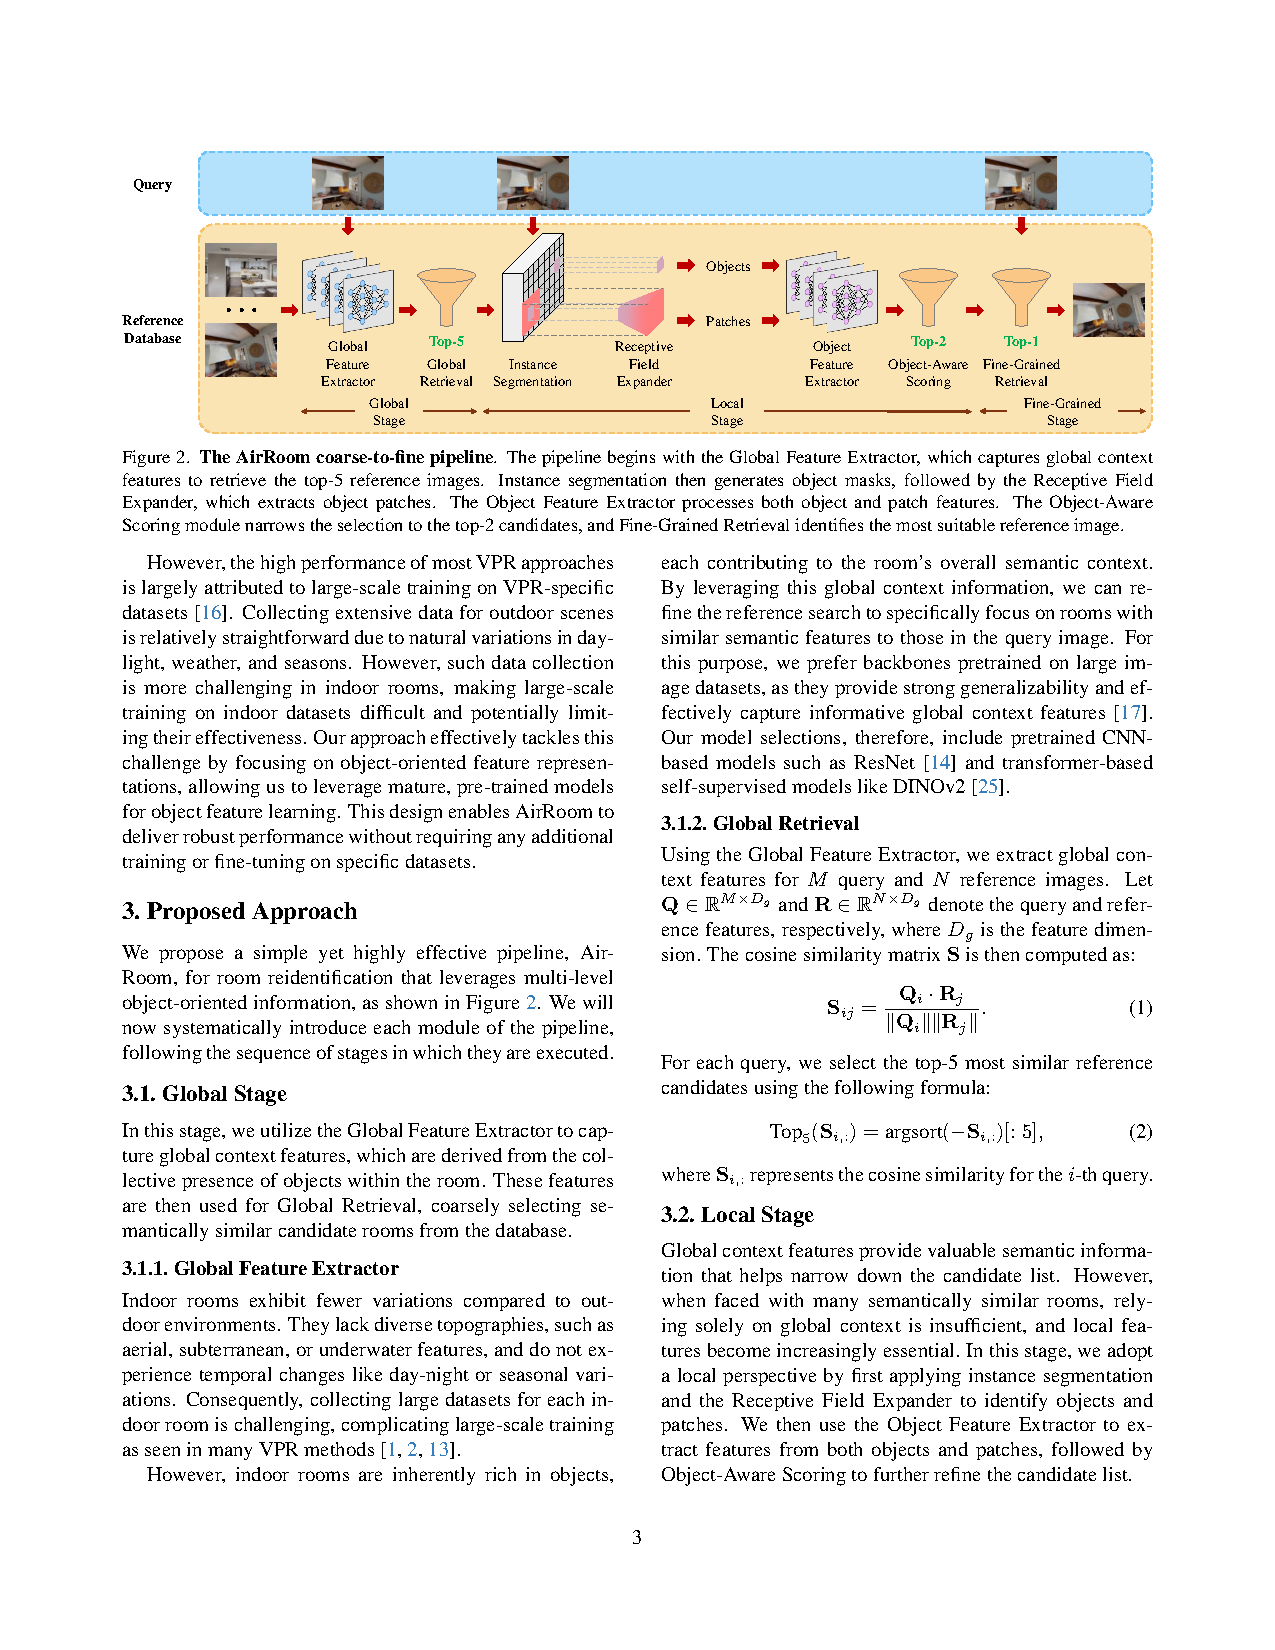
\includegraphics[width=\linewidth]{appendix_cases/case4/case4a}
        \subcaption{الجزء الأول من ملف PDF الإنجليزي للحالة 4.}
    \end{subfigure}
    \hfill
    \begin{subfigure}[t]{0.48\textwidth}
        \centering
        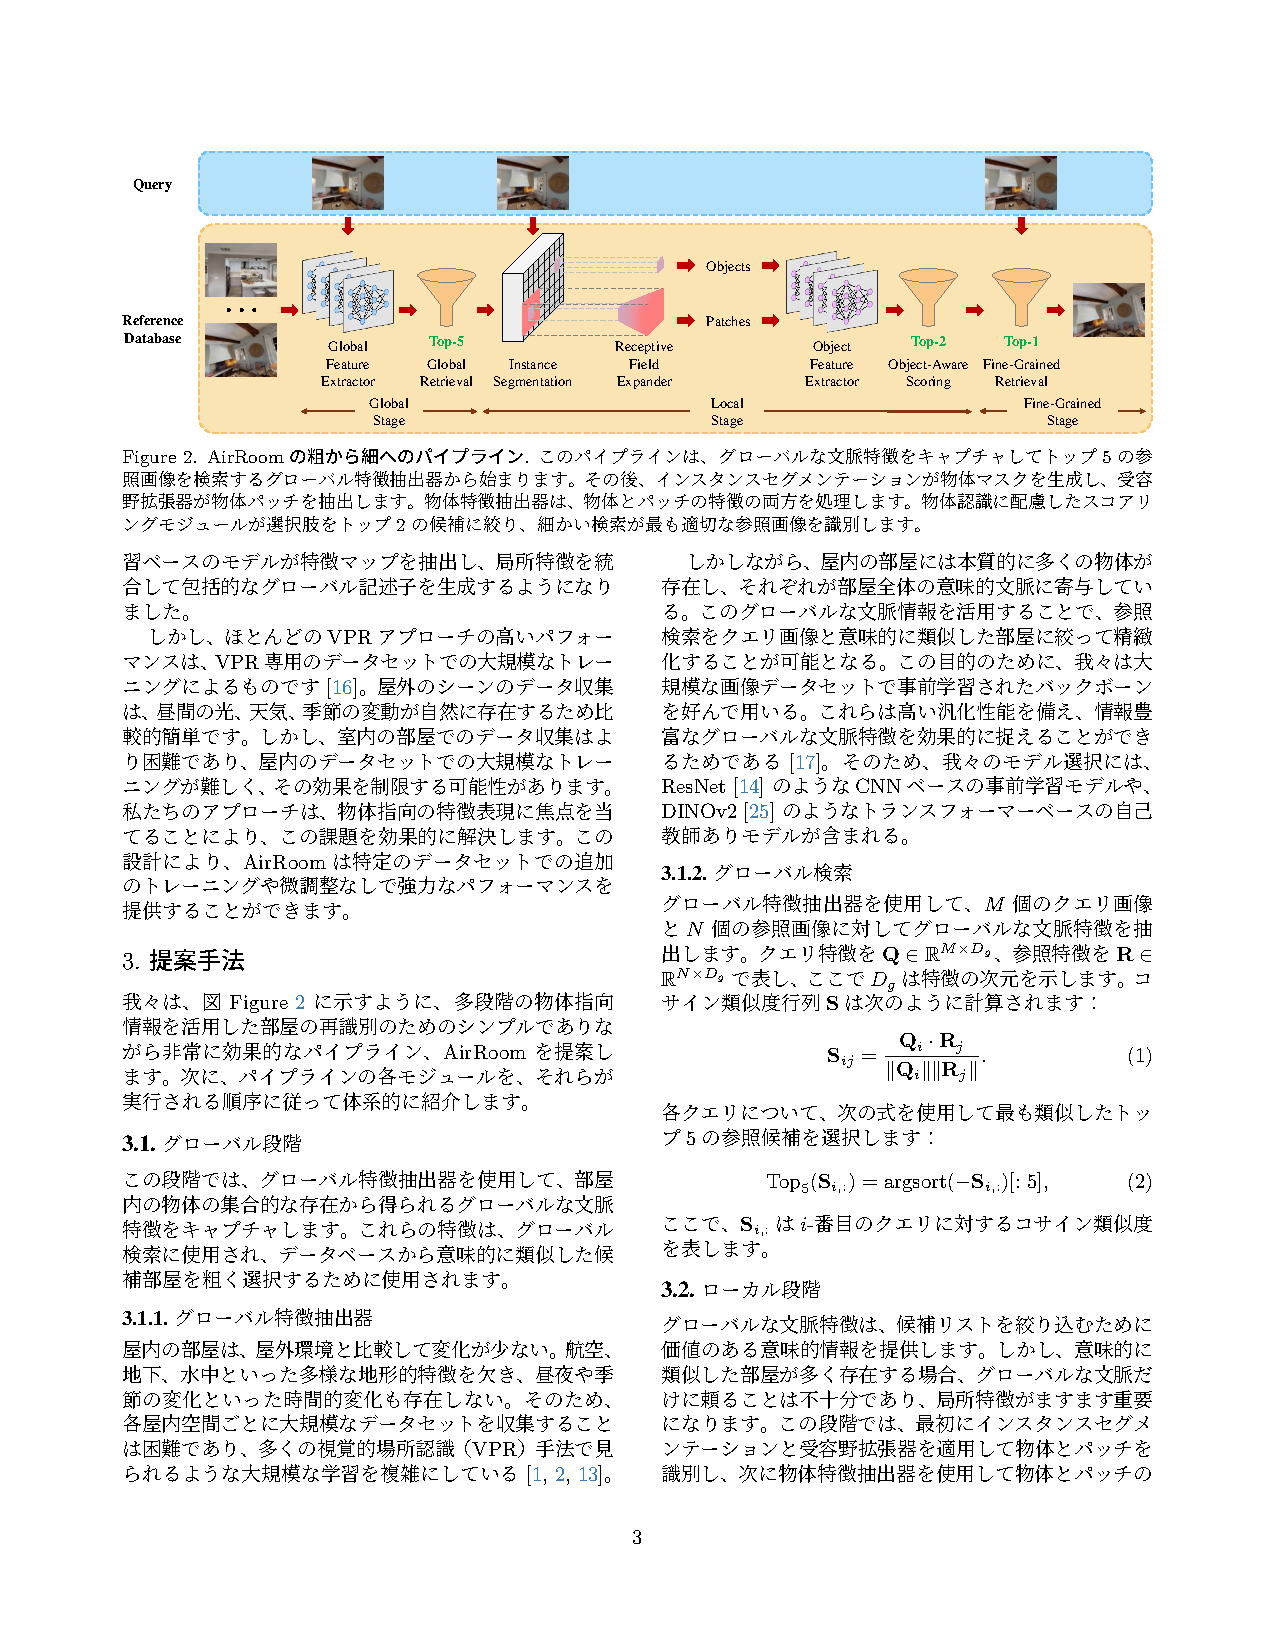
\includegraphics[width=\linewidth]{appendix_cases/case4/case4b}
        \subcaption{الجزء الأول من ملف PDF الياباني للحالة 4.}
    \end{subfigure}

    \begin{subfigure}[t]{0.48\textwidth}
        \centering
        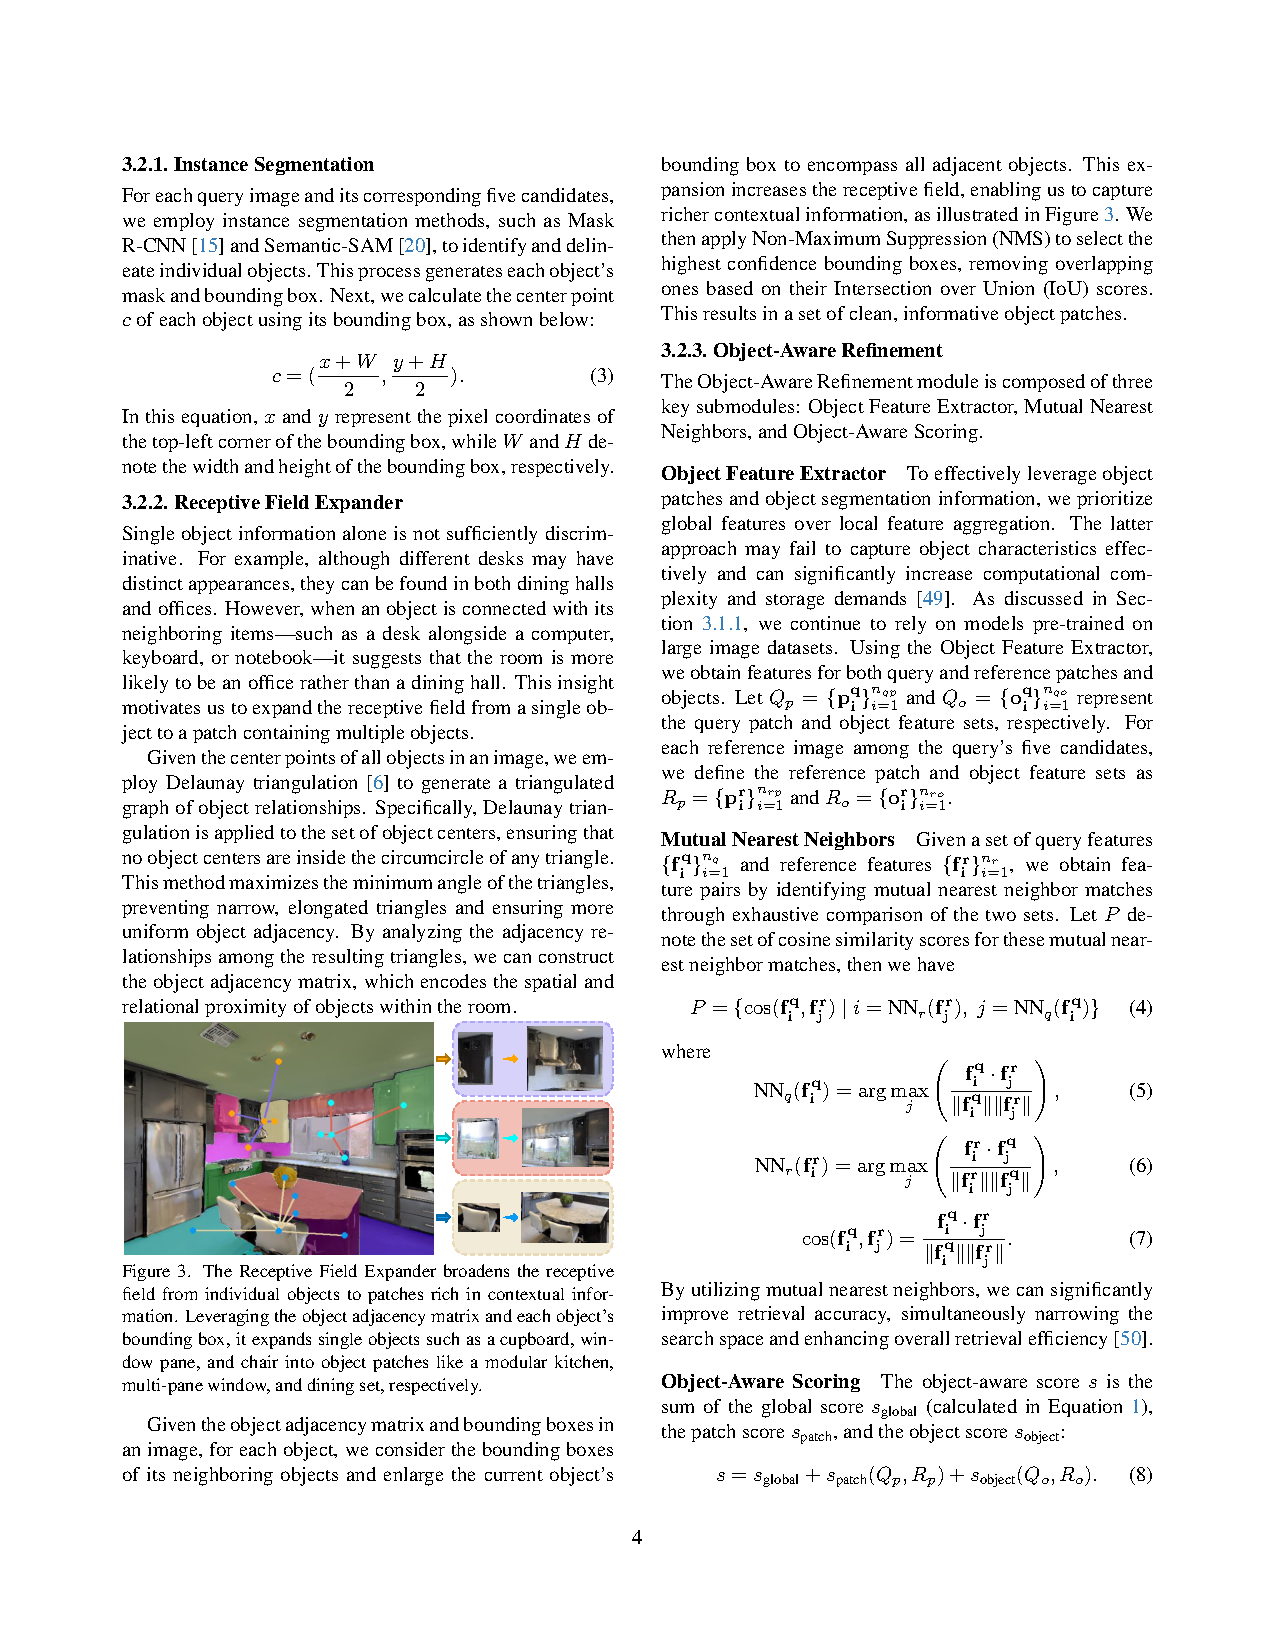
\includegraphics[width=\linewidth]{appendix_cases/case4/case4c}
        \subcaption{الجزء الثاني من ملف PDF الإنجليزي للحالة 4.}
    \end{subfigure}
    \hfill
    \begin{subfigure}[t]{0.48\textwidth}
        \centering
        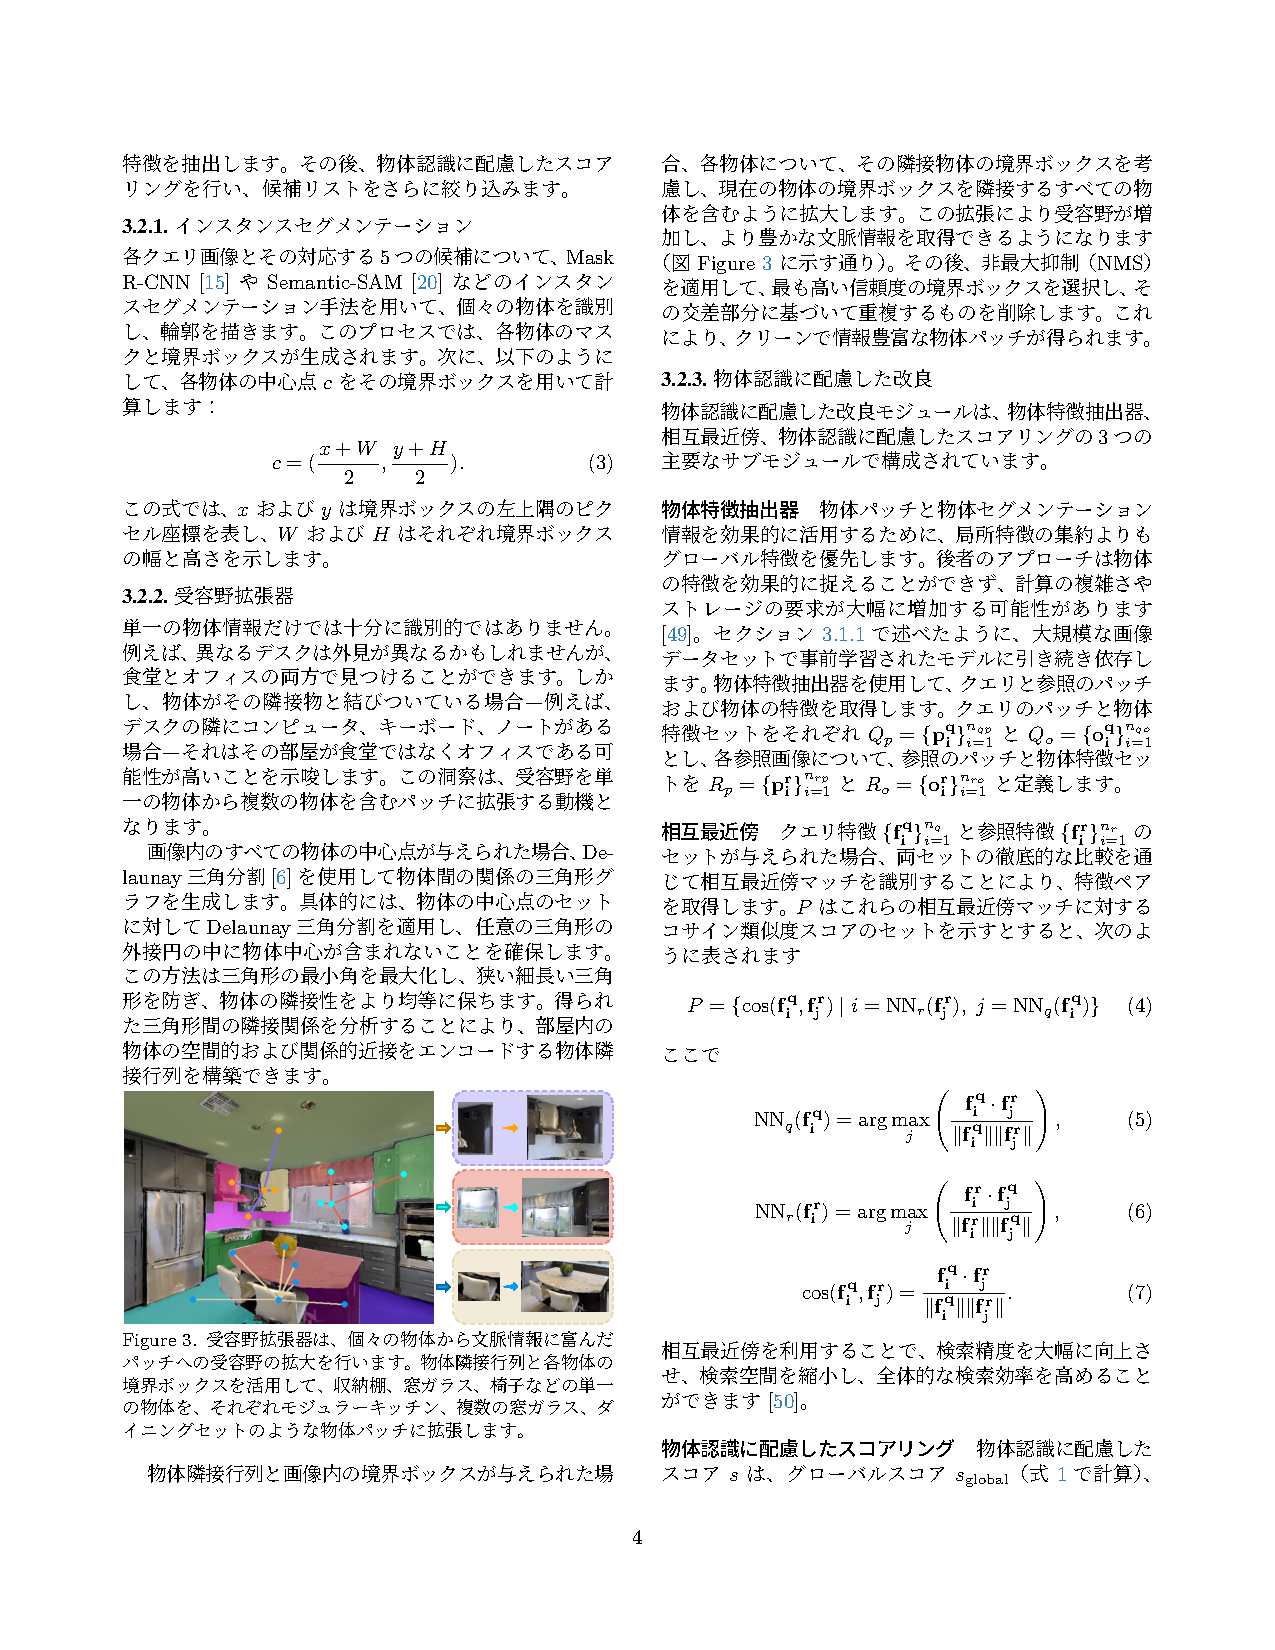
\includegraphics[width=\linewidth]{appendix_cases/case4/case4d}
        \subcaption{الجزء الثاني من ملف PDF الياباني للحالة 4.}
    \end{subfigure}

    \caption{الحالة 4 توضح أداء LaTeXTrans في مهمة En-Ja}
    \label{fig:case4}
\end{figure*}
\begin{figure*}[htbp]
    \centering

    \begin{subfigure}[t]{0.48\textwidth}
        \centering
        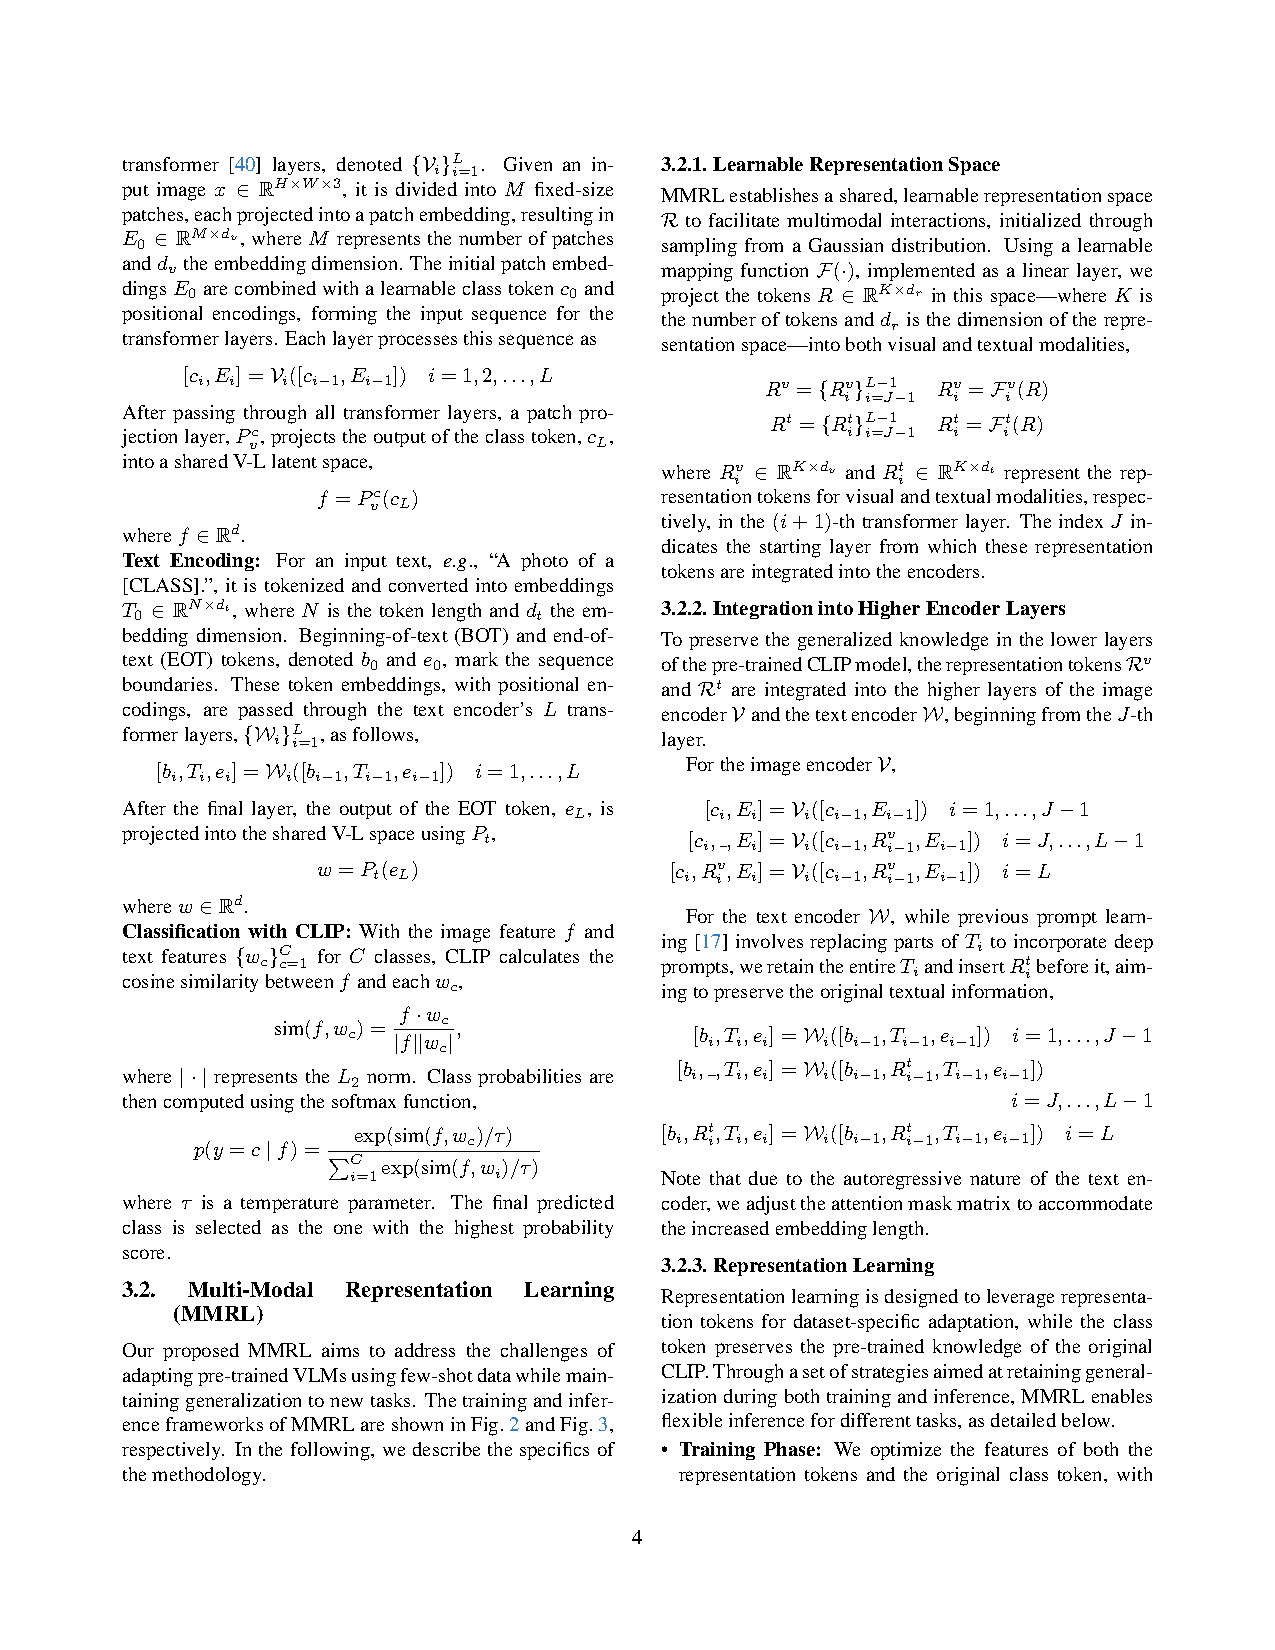
\includegraphics[width=\linewidth]{appendix_cases/case5/case5a}
        \subcaption{الجزء الأول من ملف PDF الإنجليزي للحالة 5.}
    \end{subfigure}
    \hfill
    \begin{subfigure}[t]{0.48\textwidth}
        \centering
        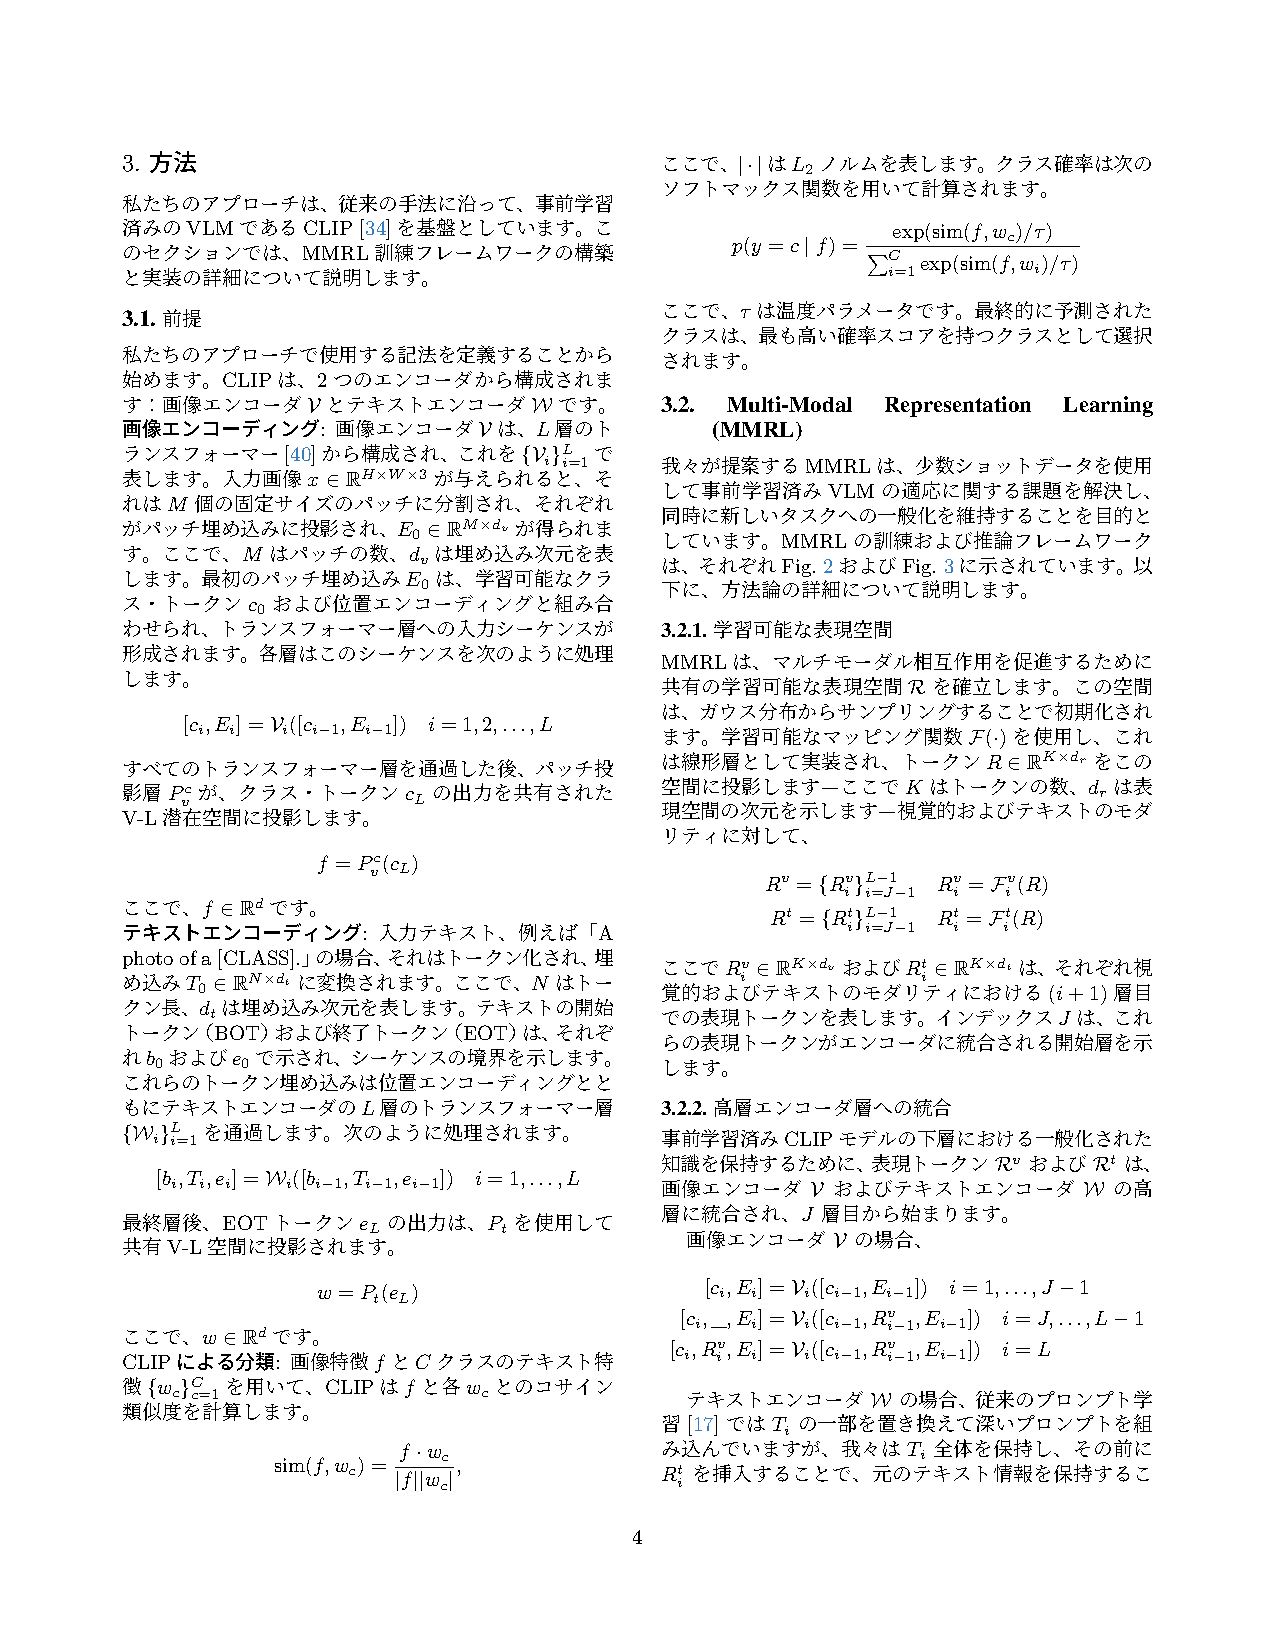
\includegraphics[width=\linewidth]{appendix_cases/case5/case5b}
        \subcaption{الجزء الأول من ملف PDF الياباني للحالة 5.}
    \end{subfigure}

    \begin{subfigure}[t]{0.48\textwidth}
        \centering
        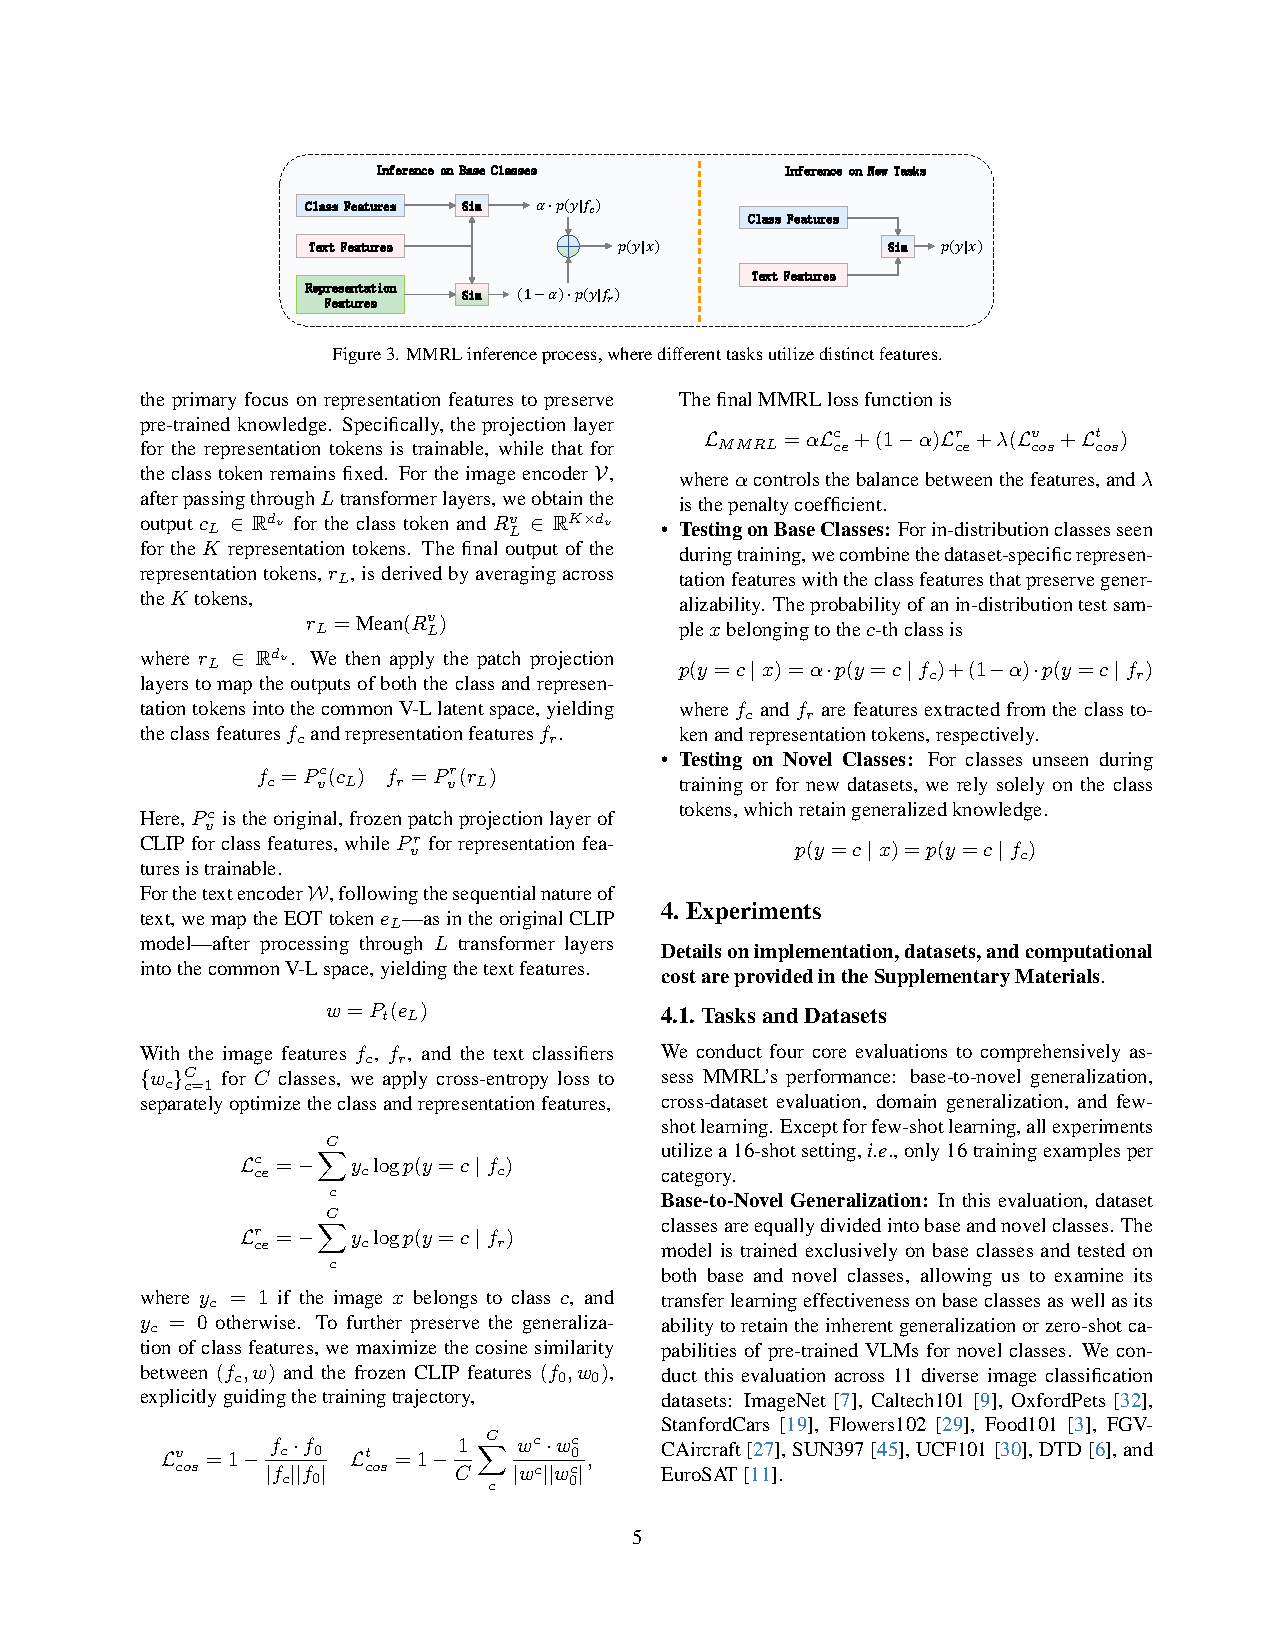
\includegraphics[width=\linewidth]{appendix_cases/case5/case5c}
        \subcaption{الجزء الثاني من ملف PDF الصيني للحالة 5.}
    \end{subfigure}
    \hfill
    \begin{subfigure}[t]{0.48\textwidth}
        \centering
        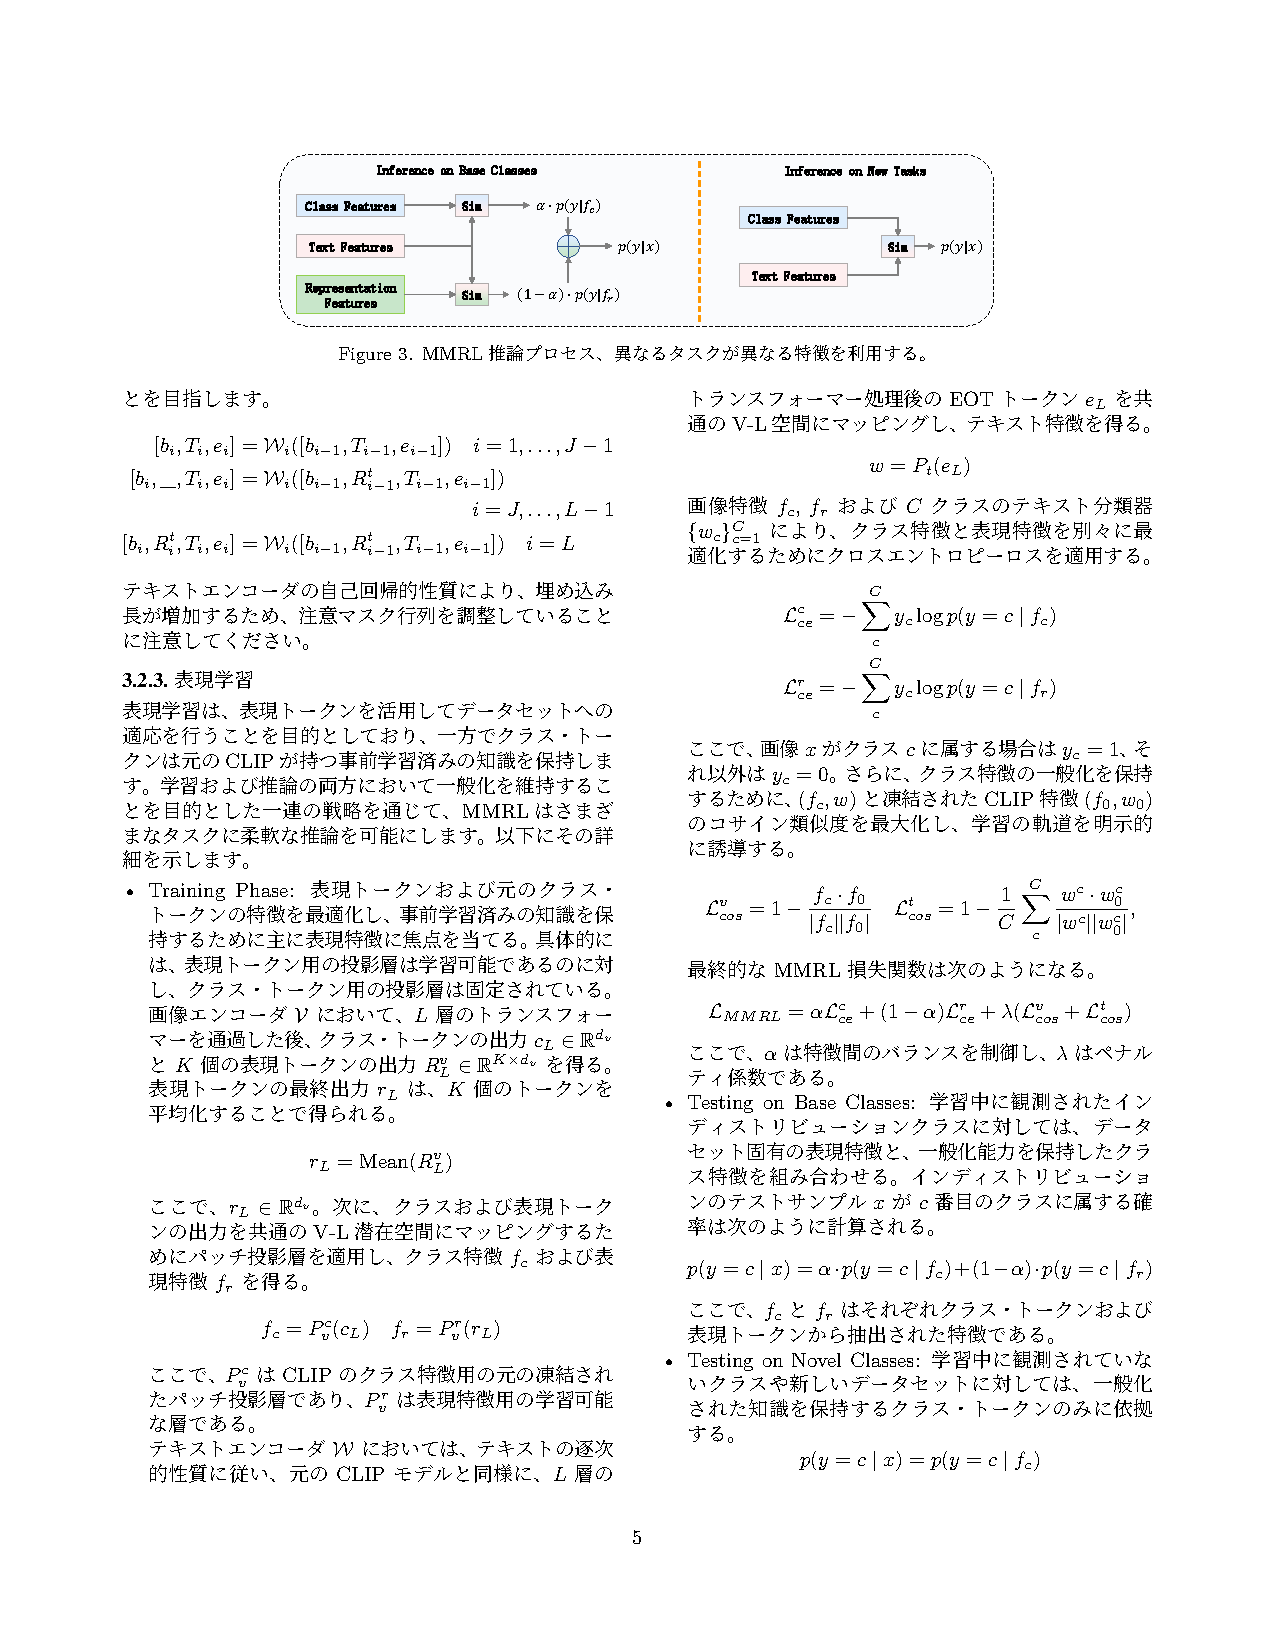
\includegraphics[width=\linewidth]{appendix_cases/case5/case5d}
        \subcaption{الجزء الثاني من ملف PDF الياباني للحالة 5.}
    \end{subfigure}

    \caption{توضح الحالة 5 أداء LaTeXTrans في مهمة En-Ja}
    \label{fig:case5}
\end{figure*}

\begin{figure*}[htbp]
    \centering

    \begin{subfigure}[t]{0.48\textwidth}
        \centering
        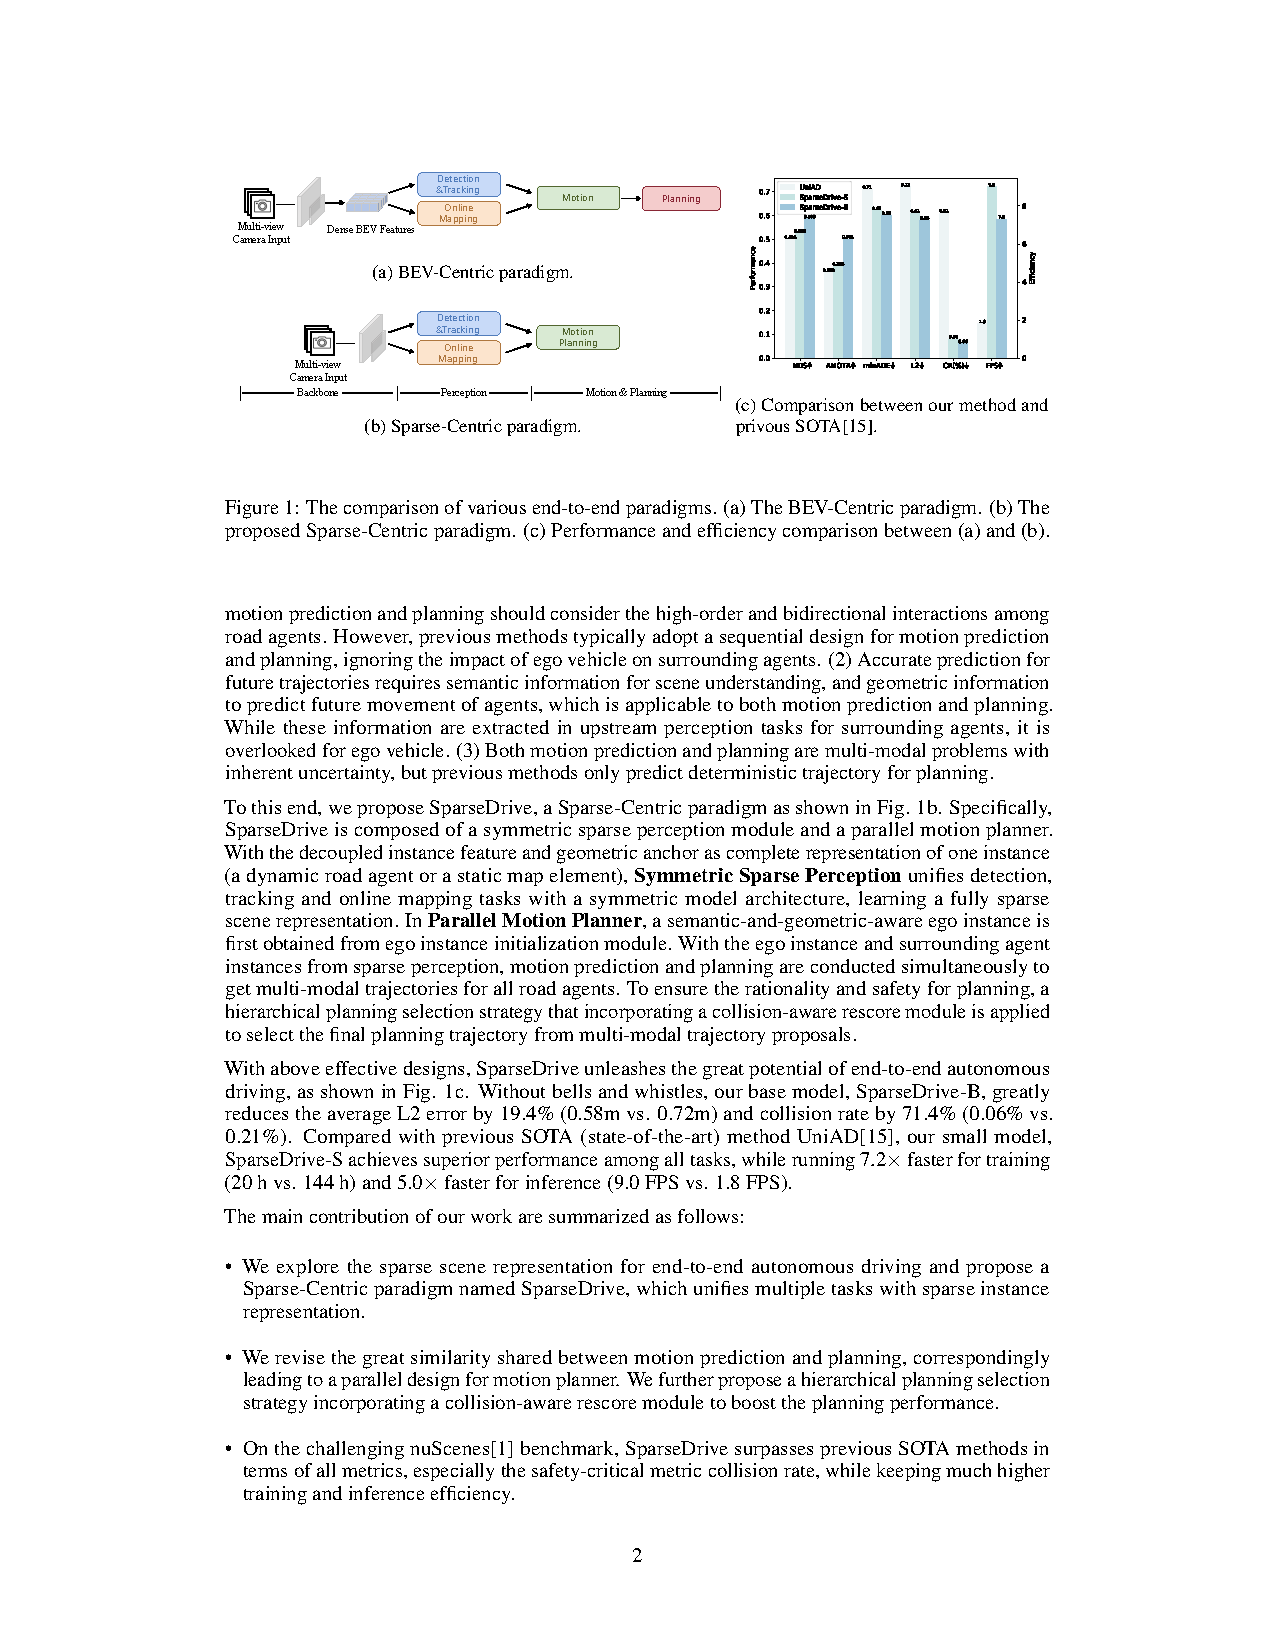
\includegraphics[width=\linewidth]{appendix_cases/case6/case6a}
        \subcaption{الجزء الأول من ملف PDF باللغة الإنجليزية للحالة 6.}
    \end{subfigure}
    \hfill
    \begin{subfigure}[t]{0.48\textwidth}
        \centering
        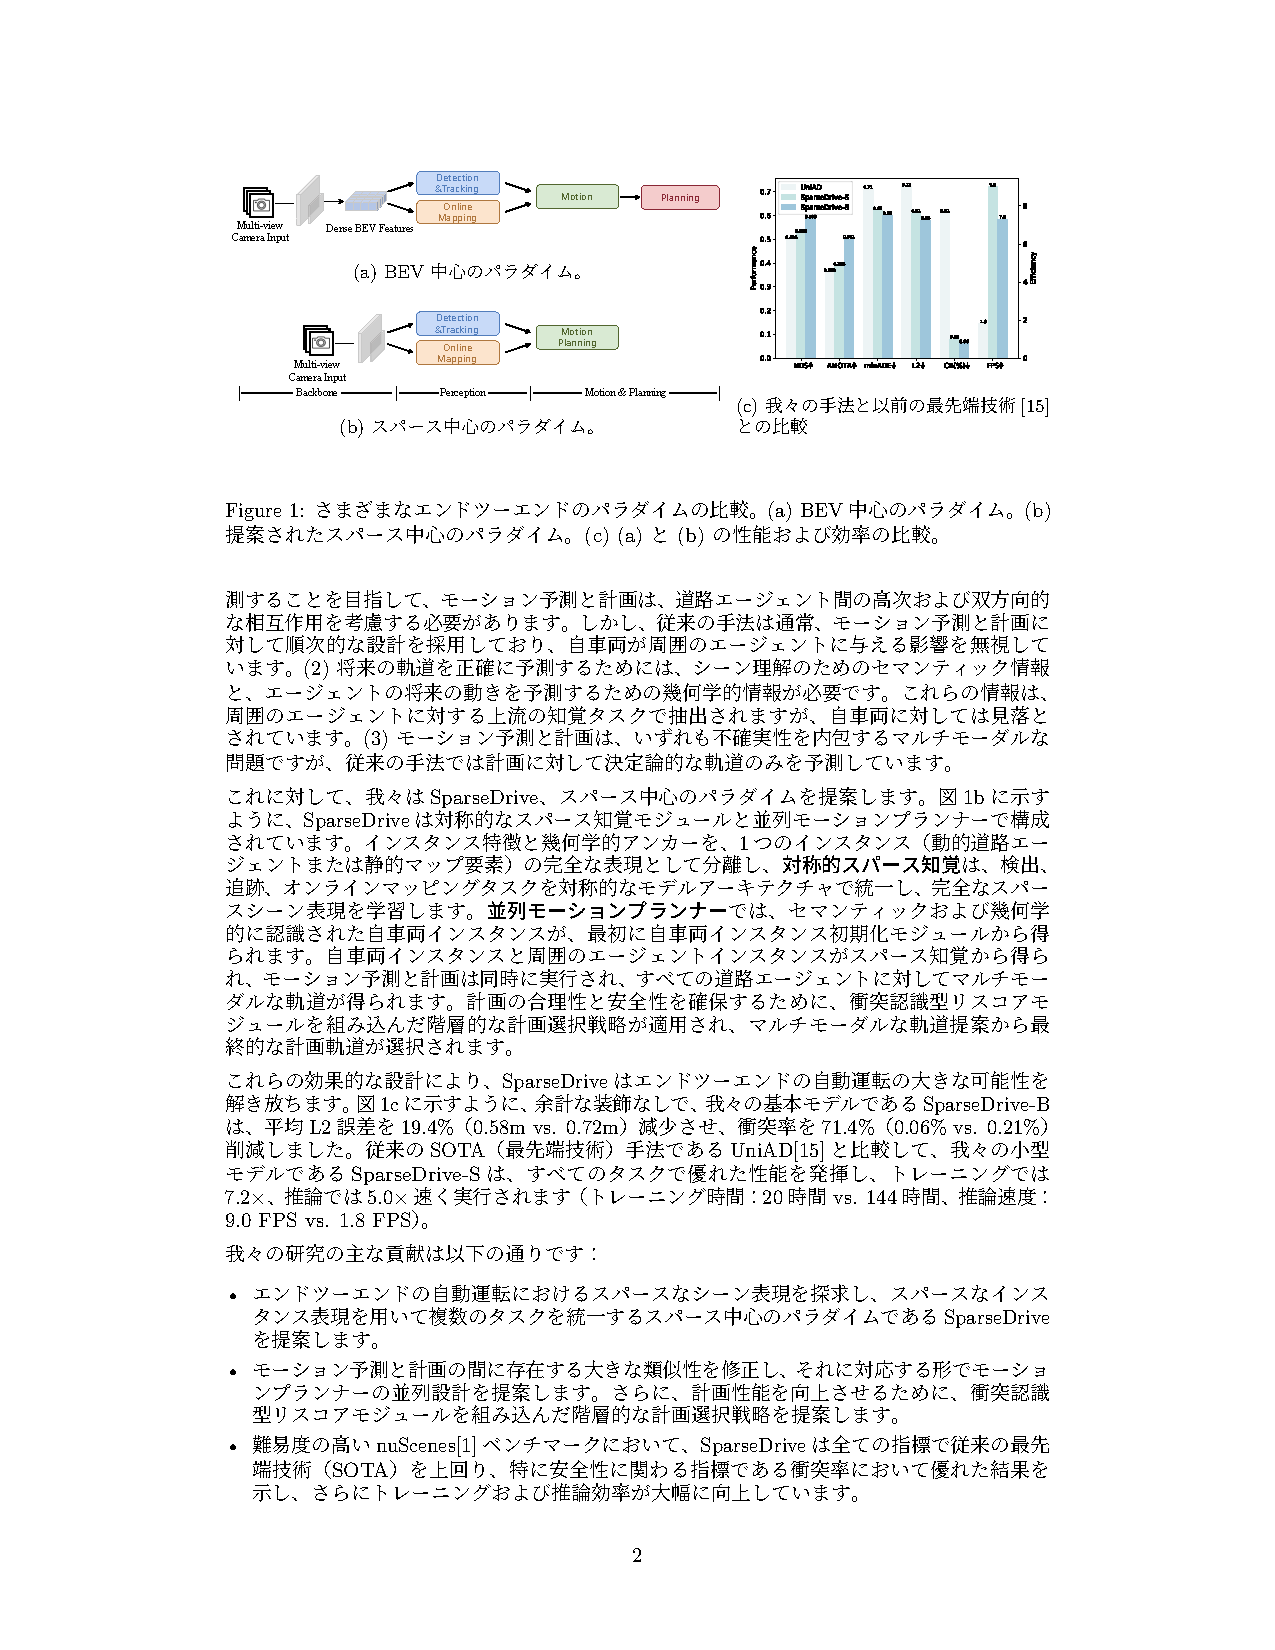
\includegraphics[width=\linewidth]{appendix_cases/case6/case6b}
        \subcaption{الجزء الأول من ملف PDF الياباني للحالة 6.}
    \end{subfigure}

    \begin{subfigure}[t]{0.48\textwidth}
        \centering
        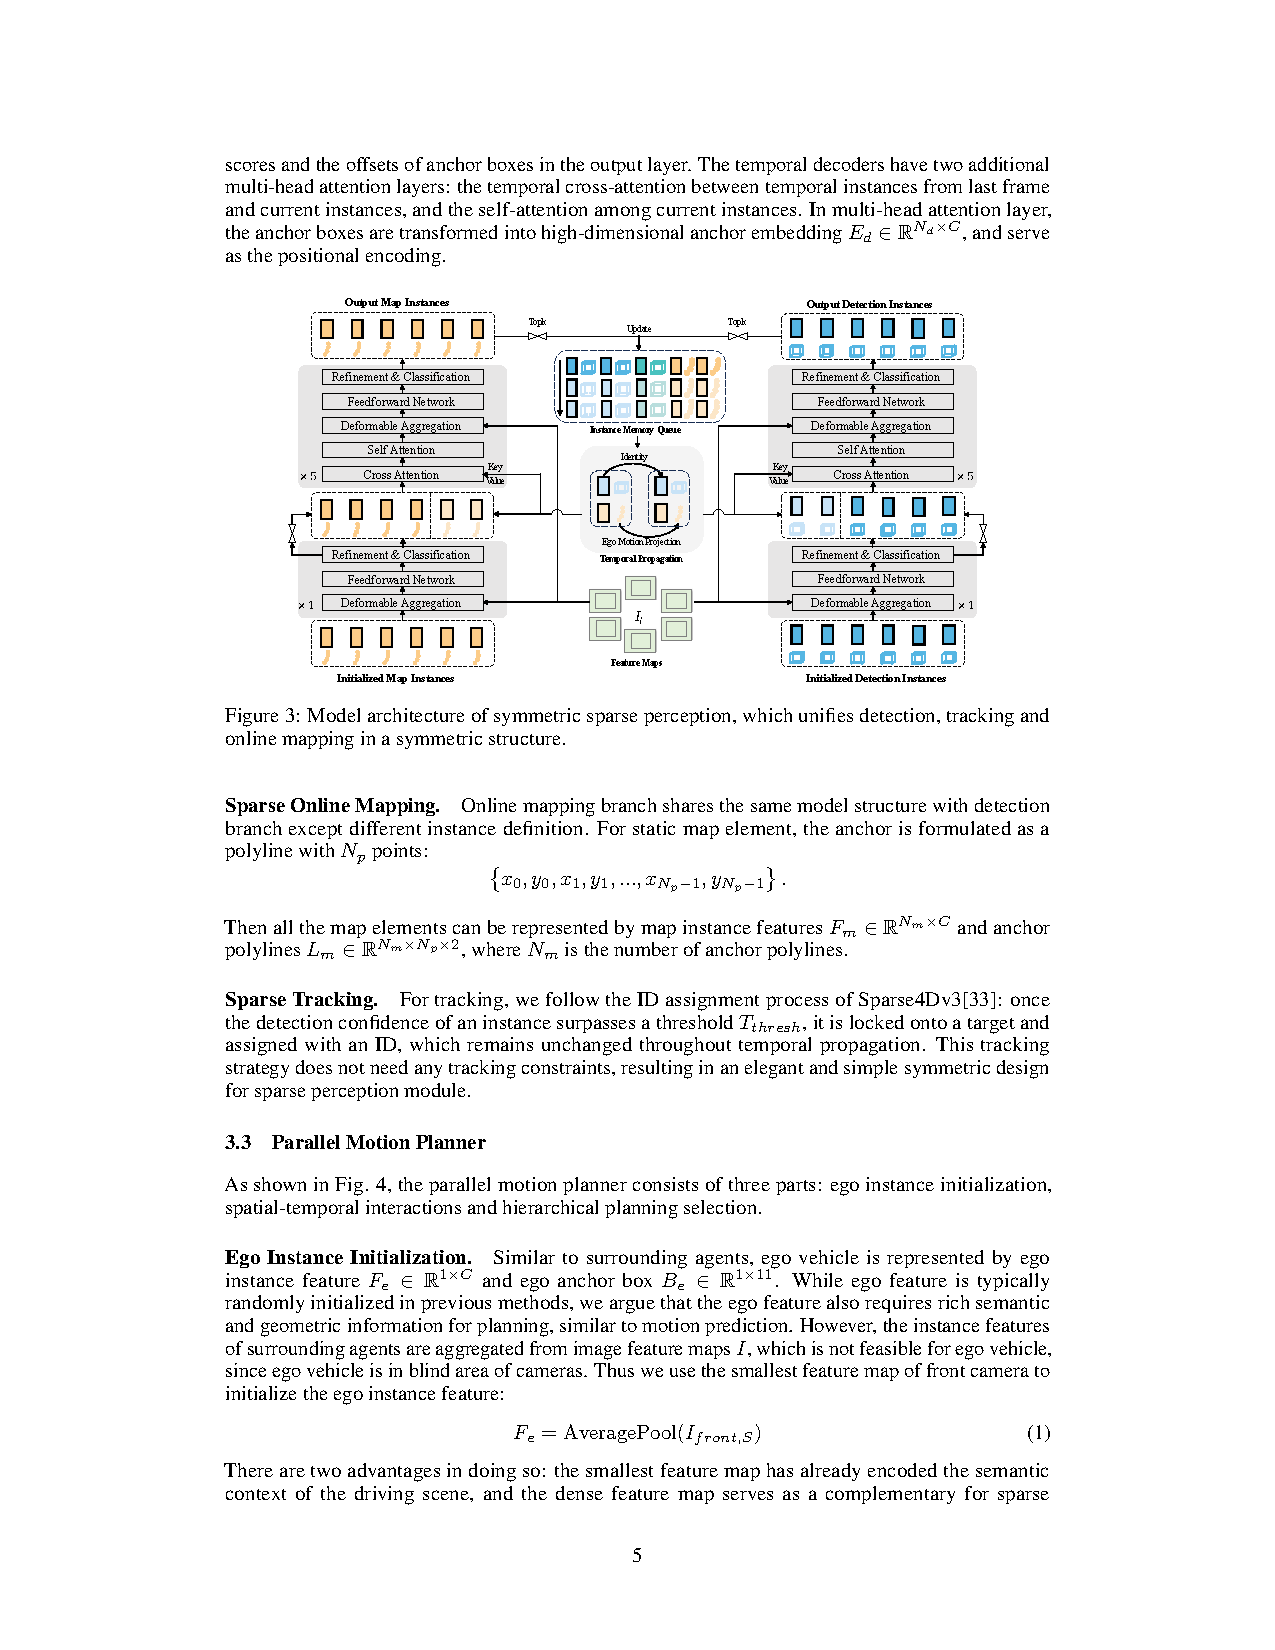
\includegraphics[width=\linewidth]{appendix_cases/case6/case6c}
        \subcaption{الجزء الثاني من ملف PDF الصيني للحالة 6.}
    \end{subfigure}
    \hfill
    \begin{subfigure}[t]{0.48\textwidth}
        \centering
        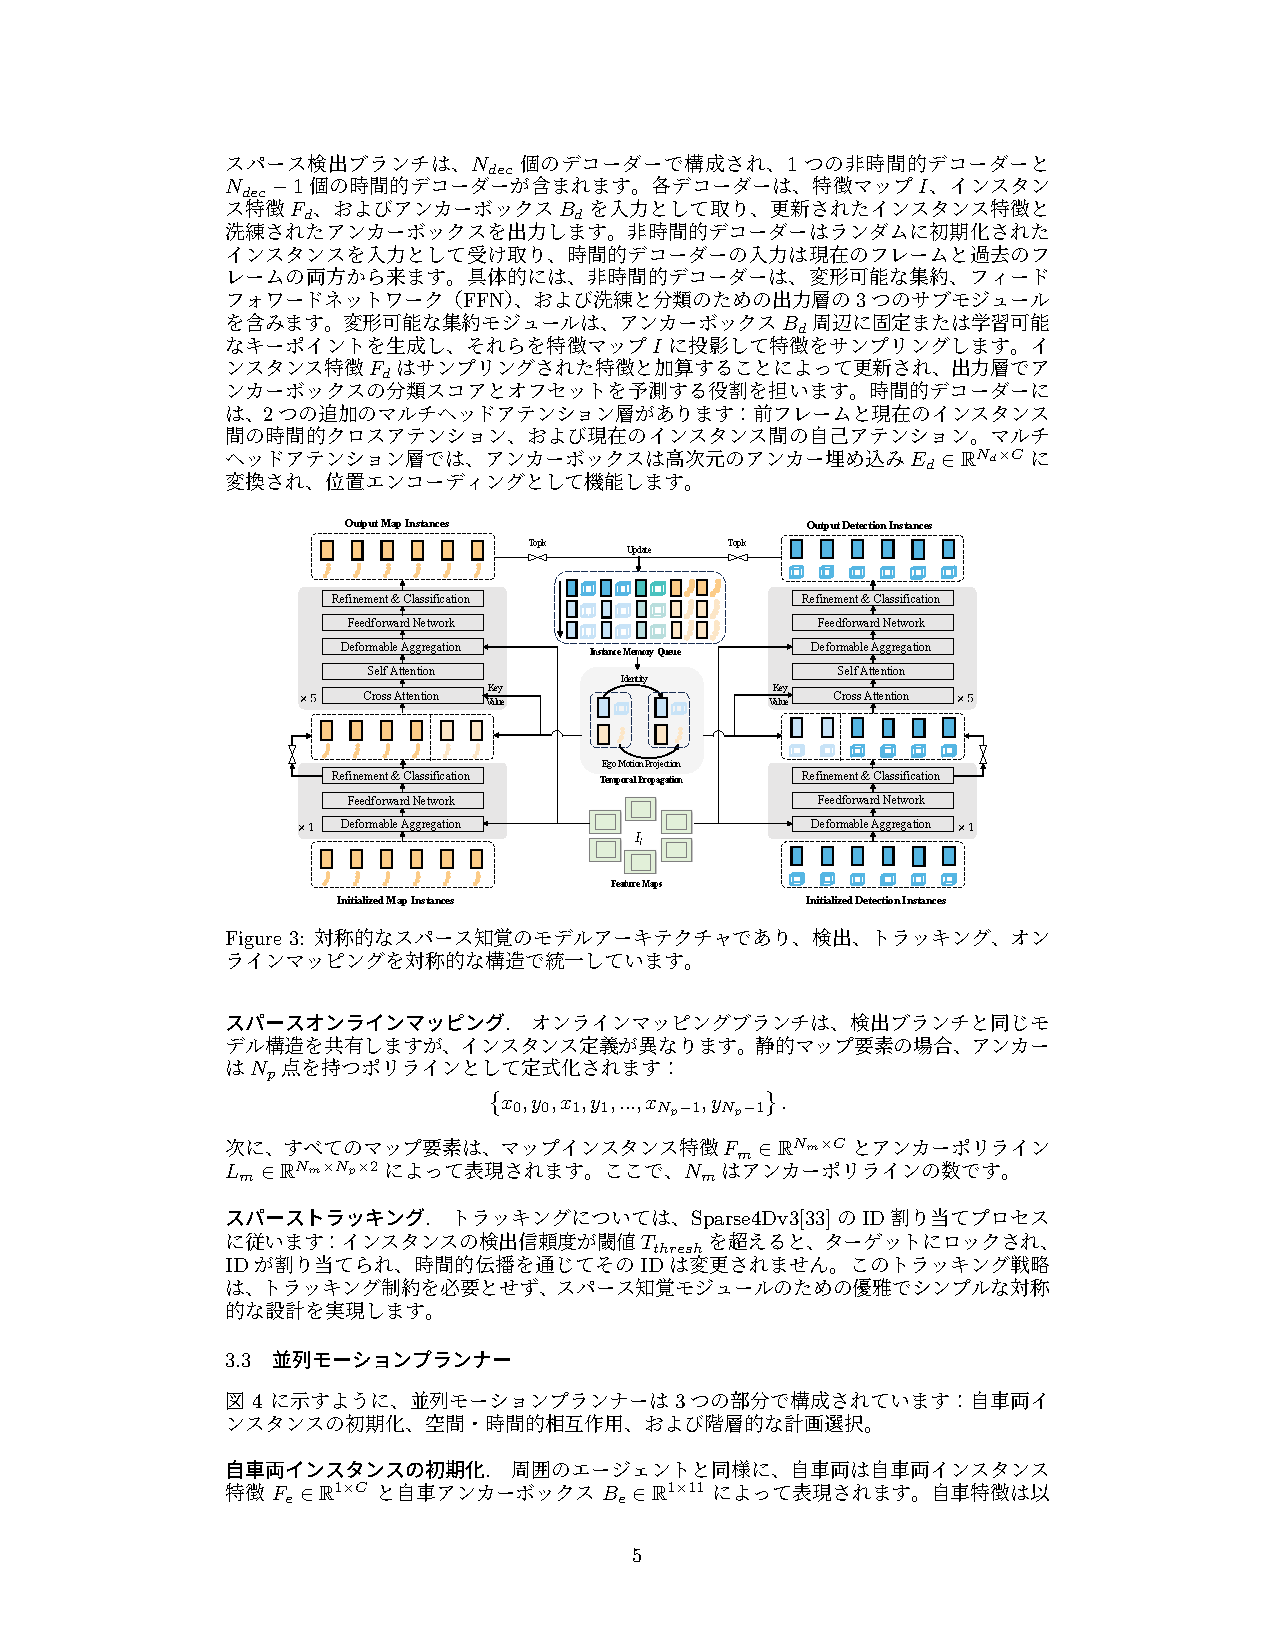
\includegraphics[width=\linewidth]{appendix_cases/case6/case6d}
        \subcaption{الجزء الثاني من ملف PDF الياباني للحالة 6.}
    \end{subfigure}

    \caption{توضح الحالة 6 أداء LaTeXTrans في مهمة En-Ja}
    \label{fig:case6}
\end{figure*}

\begin{figure*}[!t]
\centering
\begin{tcolorbox}[title=Prompt Template for LLM-score, halign=left]
\small
\ttfamily
You are a professional translation evaluator. Given an English source paragraph and its \{tgt\_language\} translation, evaluate the translation quality according to the following criteria:

\vspace{2mm}
Faithfulness: How accurately and completely does the translation convey the meaning of the source text?

Fluency: Is the translation natural, idiomatic, and grammatically correct in \{tgt\_language\}?

Terminology and Formatting Consistency: Are all technical terms translated correctly and consistently throughout the paragraph? Is the formatting—such as emphasis, symbols, references, and structural markers—preserved where applicable?

Contextual Coherence: Does the translation maintain logical flow, appropriate pronoun/reference usage, and contextual consistency across sentences within the paragraph?

\vspace{2mm}
Score each dimension from 0 to 10. Then, compute a final overall score (0 to 10), reflecting the overall translation quality, and round it to one decimal place.

Only return the final overall score as a number. Do not include explanations, sub-scores, or any additional content.

\end{tcolorbox}
    \caption{يستخدم LLM هذا الموجه، الذي يقيم وحدة ترجمة كل زوج واحدة تلو الأخرى.}
    \label{fig:llmscoreprompt}
\end{figure*}

\begin{figure*}[htbp]
    \centering
\begin{tcolorbox}[title=Prompt Template 1 for Translator, halign=left]
\small
\ttfamily
You are a professional academic translator specializing in LaTeX-based scientific writing. Your task is to translate long LaTeX texts (including section titles and content) from English to \{tgt\_language\}, while strictly maintaining the integrity of LaTeX syntax.

\vspace{2mm}
In addition to the LaTeX source, you are provided with:

1. A dynamic summary that condenses the content of all previous sections.

2. A bilingual term dictionary containing domain-specific English–\{tgt\_language\} term pairs.

\vspace{2mm}
You must use these resources to ensure translation quality:

- Use the summary to understand the document context, resolve ambiguous expressions, pronouns, or abstract references, and maintain coherence across sections.

- Strictly follow the term dictionary. If an English term in the source appears in the dictionary, you **must** use the corresponding \{tgt\_language\} translation from the dictionary without modification.

\vspace{2mm}
Please strictly follow the translation requirements below:

1. Only translate the natural language content while keeping all LaTeX commands, environments, references, mathematical expressions, and labels unchanged.

2. Section headings (e.g. natural content enclosed in \{\} in section identifiers like \texttt{\textbackslash section\{\}}, \texttt{\textbackslash subsection\{\}}, and \texttt{\textbackslash subsubsection\{\}}) must also be translated, but their LaTeX syntax must remain unchanged.

3. Do not translate or modify the following LaTeX elements:
Control commands: \texttt{\textbackslash label\{\}}, \texttt{\textbackslash cite\{\}}, \texttt{\textbackslash ref\{\}}, \texttt{\textbackslash textbf\{\}}, \texttt{\textbackslash emph\{\}}, etc.
Mathematical environments: \texttt{\$...\$}, \texttt{[...]}, \texttt{\textbackslash begin\{equation\}...\textbackslash end\{equation\}}, etc.
Any parameter or argument that includes numerical values with LaTeX layout units such as:
em, ex, in, pt, pc, cm, mm, dd, cc, nd, nc, bp, sp. Example: \texttt{\textbackslash vspace\{-1.125cm\}} or \texttt{[scale=0.58]} → leave such expressions completely unchanged.

4. Do not change the writing of special characters, such as \texttt{\textbackslash\%}, \texttt{\textbackslash\#}, \texttt{\textbackslash\&}, etc., to ensure that the translated text is accurate.

5. The final output must be a valid and compilable LaTeX document.

6. Ensure that the translated text is accurate, coherent, and follows academic writing conventions in the target language. Maintain consistent academic terminology and use standard abbreviations where appropriate.

7. Directly output only the translated LaTeX code without any additional explanations, formatting markers, or comments such as "latex".

8. \texttt{<PLACEHOLDER\_CAP\_...>}, \texttt{<PLACEHOLDER\_ENV\_...>}, \texttt{<PLACEHOLDER\_...\_begin>} and \texttt{<PLACEHOLDER\_...\_end>} are placeholders for artificial environments or captions. Please do not let them affect your translation and keep these placeholders after translation.

\vspace{2mm}
You are expected to combine semantic understanding (from the summary), precise terminology usage (from the term dictionary), and strict LaTeX fidelity to produce a high-quality translation.
\end{tcolorbox}
\caption{نموذج الطلب 1 للمترجم، يستخدم المترجم هذا الطلب لترجمة وحدة الترجمة في البداية.}
    \label{fig:translator prompt 1}
\end{figure*}

\begin{figure*}[htbp]
    \centering
\begin{tcolorbox}[title=Prompt Template 2 for Translator, halign=left]
\small
\ttfamily
You are a professional academic translator and LaTeX translation corrector.
Your task is to revise and improve machine-translated LaTeX academic texts based on three components provided by the user: the original English LaTeX source ([Original]), the existing \{tgt\_language\} translation ([Translation]), and the error information describing the issue(s) ([Error Reports]). Your revision must strictly preserve LaTeX syntax integrity and comply with the following rules.

\vspace{2mm}
1. Only translate the natural language content while keeping all LaTeX commands, environments, references, mathematical expressions, and labels unchanged.

2. Section headings (e.g. natural content enclosed in \{\} in section identifiers like \texttt{\textbackslash section\{\}}, \texttt{\textbackslash subsection\{\}}, and \texttt{\textbackslash subsubsection\{\}}) must also be translated, but their LaTeX syntax must remain unchanged.

3. Do not translate or modify the following LaTeX elements:
Control commands: \texttt{\textbackslash label\{\}}, \texttt{\textbackslash cite\{\}}, \texttt{\textbackslash ref\{\}}, \texttt{\textbackslash textbf\{\}}, \texttt{\textbackslash emph\{\}}, etc.
Mathematical environments: \texttt{\$...\$}, \texttt{[...]}, \texttt{\textbackslash begin\{equation\}...\textbackslash end\{equation\}}, etc.
Any parameter or argument that includes numerical values with LaTeX layout units such as:
em, ex, in, pt, pc, cm, mm, dd, cc, nd, nc, bp, sp. Example: \texttt{\textbackslash vspace\{-1.125cm\}} or \texttt{[scale=0.58]} → leave such expressions completely unchanged.

4. Do not change the writing of special characters, such as \texttt{\textbackslash\%}, \texttt{\textbackslash\#}, \texttt{\textbackslash\&}, etc., to ensure that the translated text is accurate.

5. The final output must be a valid and compilable LaTeX document.

6. Ensure that the translated text is accurate, coherent, and follows academic writing conventions in the target language. Maintain consistent academic terminology and use standard abbreviations where appropriate.

7. Directly output only the translated LaTeX code without any additional explanations, formatting markers, or comments such as "latex".

8. \texttt{<PLACEHOLDER\_CAP\_...>}, \texttt{<PLACEHOLDER\_ENV\_...>}, \texttt{<PLACEHOLDER\_...\_begin>} and \texttt{<PLACEHOLDER\_...\_end>} are placeholders for artificial environments or captions. Please do not let them affect your translation and keep these placeholders after translation.

\vspace{2mm}
Only output the corrected LaTeX \{tgt\_language\} translation (revised version of '[Translation]'), with all changes implemented based on the '[Original]' and '[Error]'. Do not output the original input, explanations, or any extra content.

\end{tcolorbox}
\caption{نموذج الطلب 2 للمترجم، يستخدم المترجم هذا الطلب ويجمعه مع تقارير الأخطاء المقدمة من المدقق لإعادة ترجمة وحدة الترجمة.}
    \label{fig:translation prompt 2}
\end{figure*}

\begin{figure*}[htbp]
    \centering
\begin{tcolorbox}[title=Prompt Template for Filter, halign=left]
\small
\ttfamily
You are a LaTeX translation assistant. Your task is to analyze the content inside any LaTeX environment, regardless of its environment name, and determine whether it should be translated when translating an academic paper.

Environment names can be custom-defined (e.g., 'mybox', 'resultblock', 'customalgo') and should be ignored during judgment. Only base your decision on the content itself.

\vspace{2mm}
Return 'True' if the content:

- Contains complete or partial sentences written in natural language (e.g., English), such as explanations, definitions, figure/table captions, theorem statements, or descriptions.

- Helps the reader understand the paper and would lose meaning if left untranslated.

\vspace{2mm}
Return 'False' if the content:

- Contains only code, pseudocode, mathematical formulas, drawing instructions (e.g., TikZ), formatting macros, or raw markup.

- Does not include any human-readable sentences or phrases.

\vspace{2mm}
Only output:

- 'True' or 'False'

- No explanations or additional text

\end{tcolorbox}
\caption{قالب التعليمات لفلتر، يستخدم الفلتر هذه التعليمات لتحديد ما إذا كانت وحدة الترجمة بحاجة إلى الترجمة.}
    \label{fig:filter prompt}
\end{figure*}

\begin{figure*}[htbp]
    \centering
\begin{tcolorbox}[title=Prompt Template for Terminology Extractor, halign=left]
\small
\ttfamily
You are an en-\{tgt\_language\} bilingual expert. Given an English source sentence and its corresponding \{tgt\_language\} translation, your task is to extract all domain-specific terms from the English sentence, along with their exact translations as they appear in the \{tgt\_language\} sentence.

\vspace{2mm}
These include:

- Technical terms and expressions

- Abbreviations or acronyms (e.g. RL, LM)

- Named entities or model names (e.g. COMET)

- Concept-specific noun phrases (e.g. optimization objective, long-term reward)

\vspace{2mm}
The translation must match exactly how it appears in the \{tgt\_language\} sentence. Do not invent or guess new translations.

Output the result as a list of aligned term pairs in the following format:

"<English Term>" - "<\{tgt\_language\} Translation>"

\vspace{2mm}
If there are no such terms, output: 'N/A'.

\end{tcolorbox}
\caption{قالب المطالبة لمستخرج المصطلحات، يستخدم مستخرج المصطلحات هذا القالب لاستخراج المصطلحات من كل وحدة ترجمة.}
    \label{fig:terminology Extract prompt}
\end{figure*}

\begin{figure*}
    \centering
\begin{tcolorbox}[title=Prompt Template for Summarizer, halign=left]
\small
\ttfamily
You are an academic summarization assistant designed to maintain an evolving semantic summary to support consistent and coherent machine translation of a long scientific document.

You will be given two inputs:

1. The current summary ('prev\_summary'), which reflects key information from all previously seen sections.

2. A new section of the document ('new\_section') that has not yet been summarized.

\vspace{2mm}
Your task is to:

- Integrate the new section's key content into the current summary, producing an updated summary.

- Preserve previously summarized information that remains relevant.

- Add any new findings, concepts, methods, or referential expressions introduced in the new section.

- Ensure the summary remains concise, information-dense, and suitable for machine translation context support.

- Do not repeat redundant content; merge semantically where possible.

Use clear, academic English. The updated summary should be no more than 300 words.

\end{tcolorbox}
\caption{نموذج الطلب لملخص، يستخدم الملخص هذا الطلب للحفاظ على ملخص النص السابق.}
    \label{fig:template-for-summarizer}
\end{figure*}

\end{document}
